\documentclass[a4paper,11pt]{book}
\usepackage[utf8]{inputenc}
\usepackage[spanish,es-tabla]{babel}

\usepackage{csquotes}

\decimalpoint
\usepackage{dcolumn}
\newcolumntype{.}{D{.}{\esperiod}{-1}}
\makeatletter
\addto\shorthandsspanish{\let\esperiod\es@period@code}
\makeatother

\RequirePackage{verbatim}

\usepackage{listings}
\usepackage{fancyhdr}
\usepackage{graphicx}
\usepackage{afterpage}
\usepackage{longtable}

\usepackage{subfigure}

\usepackage{amsmath}

\usepackage{eurosym}

\usepackage{lscape}

\usepackage{enumerate}
\usepackage[shortlabels]{enumitem}

\usepackage{colortbl, longtable}

\usepackage[section]{placeins}

\usepackage{tcolorbox}
%\usepackage{footnote}
%\usepackage{etoolbox}
%\BeforeBeginEnvironment{tcolorbox}{\savenotes}
%\AfterEndEnvironment{tcolorbox}{\spewnotes}

\usepackage{dsfont} 

\usepackage{hyperref}
\usepackage{xcolor}
\hypersetup{
    colorlinks,
    linkcolor={red!50!black},
    citecolor={blue!50!black},
    urlcolor={blue!80!black}
}

\newcommand{\myTitle}{Deep Reinforcement Learning para control energético eficiente de edificios\xspace}
\newcommand{\myDegree}{Máster Universitario Oficial en Ciencia de Datos e Ingeniería de Computadores\xspace}
\newcommand{\myName}{Antonio Manjavacas Lucas\xspace}
\newcommand{\myProf}{Juan Gómez Romero\xspace}
\newcommand{\myOtherProf}{Miguel Molina Solana\xspace}
\newcommand{\myFaculty}{Escuela Técnica Superior de Ingenierías Informática y de Telecomunicación\xspace}
\newcommand{\myFacultyShort}{E.T.S. de Ingenierías Informática y de Telecomunicación\xspace}
\newcommand{\myDepartment}{Departamento de Ciencias de la Computación e Inteligencia Artificial\xspace}
\newcommand{\myUni}{\protect{Universidad de Granada}\xspace}
\newcommand{\myLocation}{Granada\xspace}
\newcommand{\myTime}{\today\xspace}
\newcommand{\myVersion}{Versión 0.1\xspace}

\usepackage{url}
\usepackage{colortbl,longtable}
\usepackage[stable]{footmisc}
\usepackage{index}

\usepackage[ruled,vlined]{algorithm2e}

\usepackage{biblatex}
\addbibresource{bibliografia.bib}

\makeindex

\pagestyle{fancy}
\fancyhf{}
\fancyhead[LO]{\leftmark}
\fancyhead[RE]{\rightmark}
\fancyhead[RO,LE]{\textbf{\thepage}}

\renewcommand{\chaptermark}[1]{\markboth{\textbf{#1}}{}}
\renewcommand{\sectionmark}[1]{\markright{\textbf{\thesection. #1}}}

\setlength{\headheight}{1.5\headheight}

\newcommand{\HRule}{\rule{\linewidth}{0.5mm}}

% Utilizar con \begin{teorema} \end{teorema} ...
\newtheorem{teorema}{Teorema}[chapter]
\newtheorem{ejemplo}{Ejemplo}[chapter]
\newtheorem{definicion}{Definición}[chapter]

% Minimizar fragmentacion de codigo
\lstnewenvironment{listing}[1][]
   {\lstset{#1}\pagebreak[0]}{\pagebreak[0]}

\newcommand{\bigrule}{\titlerule[0.5mm]}

% Evitar que en las páginas en blanco se muestren las cabeceras
\makeatletter
\def\clearpage{%
  \ifvmode
    \ifnum \@dbltopnum =\m@ne
      \ifdim \pagetotal <\topskip
        \hbox{}
      \fi
    \fi
  \fi
  \newpage
  \thispagestyle{empty}
  \write\m@ne{}
  \vbox{}
  \penalty -\@Mi
}
\makeatother

\usepackage{pdfpages}

%%%%%%%% algorithm2e - spanish %%%%%%%%
\renewcommand{\listalgorithmcfname}{Índice de algoritmos}%
\renewcommand{\algorithmcfname}{Algoritmo}%
\SetKwInput{KwIn}{Entrada}%
\SetKwInput{KwOut}{Salida}%
\SetKwInput{KwResult}{Resultado}%
\SetKw{KwRet}{devuelve}%
\SetKw{Return}{devolver}%
\SetKwBlock{Begin}{Inicio}{fim}%
\SetKwRepeat{Repeat}{repetir}{mientras que}%
\SetKwIF{If}{ElseIf}{Else}{si}{entonces}{si no si}{si no}{fin si}%
\SetKwFor{For}{para}{fa\c{c}a}{fim para}%
\SetKwFor{ForEach}{para cada}{hacer}{fin para cada}%
\SetKwFor{While}{mientras}{hacer}{fin mientras}%

\begin{document}


\setcounter{tocdepth}{4}

\begin{titlepage}
 
 
\newlength{\centeroffset}
\setlength{\centeroffset}{-0.5\oddsidemargin}
\addtolength{\centeroffset}{0.5\evensidemargin}
\thispagestyle{empty}

\noindent\hspace*{\centeroffset}\begin{minipage}{\textwidth}

\centering

\includegraphics[width=0.9\textwidth]{imagenes/logo_ugr.png}\\[1.4cm]

\textsc{ \Large TRABAJO FIN DE MÁSTER\\[0.2cm]}
\textsc{ MÁSTER UNIVERSITARIO OFICIAL EN CIENCIA DE DATOS E INGENIERÍA DE COMPUTADORES}\\[1cm]

{\LARGE\bfseries Deep Reinforcement Learning para control energético eficiente de edificios\\
}
\end{minipage}

\vspace{1.5cm}
\noindent\hspace*{\centeroffset}\begin{minipage}{\textwidth}
\centering

\textbf{Autor}\\ {Antonio Manjavacas Lucas}\\[2.5ex]
\textbf{Directores}\\
{Juan Gómez Romero\\
Miguel Molina Solana}\\[2cm]

\includegraphics[width=0.4\textwidth]{imagenes/logo_etsiit.png}\\[0.1cm]
\textsc{Escuela Técnica Superior de Ingenierías Informática y de Telecomunicación}\\
\textsc{---}\\
Granada, \today
\end{minipage}


\end{titlepage}



\chapter*{}

\begin{titlepage}
 
\setlength{\centeroffset}{-0.5\oddsidemargin}
\addtolength{\centeroffset}{0.5\evensidemargin}
\thispagestyle{empty}

\noindent\hspace*{\centeroffset}\begin{minipage}{\textwidth}

\centering

\vspace{3.3cm}


\includegraphics[scale=0.2]{imagenes/logo_energym.png} 
\vspace{0.5cm}

% Title

{\LARGE\bfseries Deep Reinforcement Learning para control energético eficiente de edificios\\
}
\end{minipage}

\vspace{2.5cm}
\noindent\hspace*{\centeroffset}\begin{minipage}{\textwidth}
\centering

\textbf{Autor}\\ {Antonio Manjavacas Lucas}\\[2.5ex]
\textbf{Directores}\\
{Juan Gómez Romero\\
Miguel Molina Solana}\\[2cm]
\end{minipage}
\vspace{\stretch{2}}

\end{titlepage}




\cleardoublepage
\thispagestyle{empty}

\begin{center}
{\large\bfseries Deep Reinforcement Learning para control energético eficiente de edificios}\\
\end{center}
\begin{center}
Antonio Manjavacas Lucas\\
\end{center}

\noindent{\textbf{Palabras clave}: Aprendizaje profundo por refuerzo; Control energético de edificios; Agentes inteligentes}\\

\vspace{0.7cm}
\noindent{\textbf{Resumen}}\\

En las últimas décadas, tanto el calentamiento global como el cambio climático se han visto significativamente afectados por el incremento de la demanda energética de edificios residenciales y comerciales. Estos son responsables de un tercio del consumo mundial de energía y de hasta un 40\% de las emisiones de CO$_2$, mayormente producidas por los sistemas de calefacción, ventilación y aire acondicionado (HVAC) destinados a garantizar el bienestar de sus ocupantes.

Ante esta problemática, optimizar el control de los sistemas HVAC se plantea como una solución necesaria ante el creciente interés por garantizar la eficiencia energética de los edificios. Dicho control ha sido tradicionalmente llevado a cabo mediante técnicas reactivas, las cuales no siempre garantizan la maximización del confort de los ocupantes y, al mismo tiempo, la minimización del consumo energético a largo plazo.

En contraposición a estos métodos tradicionales, en los últimos años ha aumentado el interés por las técnicas basadas en aprendizaje profundo por refuerzo (DRL) orientadas a control HVAC, a raíz de los resultados exitosos en otras áreas, como la robótica o los juegos. No obstante, se trata de un campo relativamente inmaduro, donde se carece de marcos de referencia y bancos de prueba específicamente destinados a reproducir y comparar los diferentes algoritmos que conforman el estado del arte.

En respuesta a esta necesidad, el objetivo perseguido en este trabajo será el desarrollo de un entorno de ejecución de simulaciones energéticas orientado al uso y evaluación de diferentes algoritmos de DRL en control HVAC. A su vez, se profundizará en la experimentación con estos algoritmos haciendo uso del entorno implementado, evaluando los resultados obtenidos en términos de consumo energético y confort.

\cleardoublepage
\thispagestyle{empty}

\begin{center}
{\large\bfseries Deep Reinforcement Learning for efficient building energy control}\\
\end{center}
\begin{center}
Antonio Manjavacas Lucas\\
\end{center}

\noindent{\textbf{Keywords}: Deep Reinforcement Learning; Building energy control; Intelligent agents}\\

\vspace{0.7cm}
\noindent{\textbf{Abstract}}\\

In recent decades, both global warming and climate change have been significantly affected by the increased energy demand of residential and commercial buildings. These are responsible for one third of global energy consumption and up to 40\% of CO$_2$ emissions, mostly produced by heating, ventilation and air conditioning (HVAC) systems designed to ensure the well-being of their occupants.

Given this problem, optimizing the control of HVAC systems is a necessary solution in view of the growing interest in guaranteeing the energy efficiency of buildings. This control has traditionally been carried out by means of reactive techniques, which do not always guarantee the maximization of occupants' comfort and, at the same time, the long-term minimization of energy consumption.

In contrast to these traditional methods, in recent years there has been a growing interest in deep reinforcement learning (DRL) techniques for HVAC control, following successful results in other areas such as robotics or games. However, this is a relatively immature field, where there is a lack of reference frameworks and benchmarks specifically aimed at reproducing and comparing the different algorithms that comprise the state of the art.

As a response to this need, the objective of this work will be the development of an environment for the execution of energy simulations oriented to the use and evaluation of different DRL algorithms in HVAC control. At the same time, the experimentation with these algorithms using the implemented environment will be deepened, evaluating the results obtained in terms of energy consumption and comfort.

\chapter*{}
\thispagestyle{empty}

Yo, \textbf{Antonio Manjavacas}, alumno de la titulación Máster Universitario Oficial en Ciencia de Datos e Ingeniería de Computadores de la \textbf{Escuela Técnica Superior
de Ingenierías Informática y de Telecomunicación de la Universidad de Granada}, con DNI \textbf{06286831B}, autorizo la ubicación de la siguiente copia de mi Trabajo Fin de Máster en la biblioteca del centro para que pueda ser
consultada por las personas que lo deseen.

\vspace{6cm}

\begin{center}
    \noindent Antonio Manjavacas Lucas
\end{center}

\vspace{2cm}

\begin{flushright}
Granada a \today .
\end{flushright}

\chapter*{}
\thispagestyle{empty}

D. \textbf{Juan Gómez Romero}, profesor titular del Departamento Ciencias de la Computación e Inteligencia Artificial de la Universidad de Granada.

\vspace{0.5cm}

D. \textbf{Miguel Molina Solana}, profesor ayudante doctor del Departamento Ciencias de la Computación e Inteligencia Artificial de la Universidad de Granada.

\vspace{0.5cm}

\textbf{Informan:}

\vspace{0.5cm}

Que el presente trabajo, titulado \textit{\textbf{Deep Reinforcement Learning para control energético eficiente de edificios}}, ha sido realizado bajo su supervisión por \textbf{Antonio Manjavacas Lucas}, y autorizan la defensa de dicho trabajo ante el tribunal que corresponda.

\vspace{0.5cm}

Y para que conste, expiden y firman el presente informe en Granada a \today.

\vspace{1cm}

\textbf{Los directores:}

\vspace{5cm}

\begin{center}
    \noindent \textbf{Juan Gómez Romero \ \ \ \ \ Miguel Molina Solana}
\end{center}

\chapter*{Agradecimientos}
\thispagestyle{empty}

\vspace{1cm}

Quisiera dar las gracias y dedicar este trabajo a todas las personas que, desde lo personal como lo profesional, me han acompañado a lo largo de este maravilloso año, repleto de aprendizaje y buenas experiencias.

Gracias a Juan y Miguel, por su cercanía y sus buenos consejos, así como por brindarme la oportunidad de colaborar en este proyecto y profundizar en mi pasión por el aprendizaje por refuerzo, un campo que me apasiona y del que nunca dejaré de aprender. 

Este trabajo tampoco habría sido posible sin la ayuda incondicional de Alejandro y Javier, compañeros de trabajo, reuniones, mensajes de Slack y satisfacciones por ver crecer esta iniciativa. En palabras de Javier: ``hace unos meses parecía algo muy lejano''. ¡Gracias por todo!

También quisiera agradecer a mis padres, Antonio y Criptana, todo su sacrificio y ánimo a lo largo de un año marcado por la distancia. Gracias por entender lo que me hace feliz y prestarme todo vuestro apoyo.

Gracias a Andrea, Ithiel, Patricio, Margarita y Anouk, compañeros a lo largo de un viaje que comenzó en diciembre y terminó en La Gomera. Seguro que volveremos a encontrarnos.

A mis buenos amigos \textit{granaínos} y no tan \textit{granaínos}: Carlos, Mape, Eva, Elena, Jose, Pablo, Juanje, Blanca... ¡sois muchos los que habéis hecho de este un año inigualable! Gracias, de corazón, por todos los buenos momentos y experiencias compartidas.

Por último, pero no menos importante, quisiera dar las gracias a Laura y Virginia. Jamás pensé que en un año marcado por la pandemia y la ``distancia social'' me acercaría tanto a dos personas tan maravillosas. Gracias por soportarme, ser testigos de mi trabajo y estar ahí en los buenos y malos momentos. 

\begin{flushright}
\textit{Antonio Manjavacas Lucas\\
Granada, 27 de junio de 2021}
\end{flushright}


\frontmatter
\tableofcontents
\listoffigures
\listoftables
\listofalgorithms

\mainmatter
\setlength{\parskip}{5pt}

%% Capitulos

\chapter{Introducción}
\label{ch:1}

En este primer capítulo, se dará a conocer la motivación del proyecto, ofreciendo una perspectiva general del contexto y objetivos que lo atañen.

\section{Motivación}

En las últimas décadas, tanto el calentamiento global como el cambio climático se han visto  significativamente alentados por el crecimiento en la demanda energética de edificios residenciales y comerciales. De acuerdo con organizaciones como la Agencia Internacional de Energía\footnote{\url{https://www.iea.org/topics/buildings}} (\textit{International Energy Agency}, IEA), o WBCSD\footnote{\url{https://www.wbcsd.org/Programs/Cities-and-Mobility/Resources/Business-realities-and-opportunities-Summary}} (\textit{World Business Council for Sustainable Development}), los edificios y el sector de la construcción son responsables de más de un tercio del consumo mundial de energía, y de hasta un 40\% del total de las emisiones directas e indirectas de CO$_2$. 

Dichas emisiones, tras cierta estabilidad entre 2013 y 2016, alcanzaron su mayor nivel jamás registrado en 2019, produciéndose un crecimiento propiciado por múltiples factores, tales como la creciente demanda de energía destinada a sistemas de calefacción, ventilación y aire acondicionado (HVAC), el uso extendido de combustibles fósiles, la falta de políticas eficaces en eficiencia energética, así como una insuficiente inversión en edificios sostenibles\footnote{\url{https://www.iea.org/reports/tracking-buildings-2020}}.

Ante esta problemática, las propuestas más recientes destinadas a favorecer la eficiencia energética abogan, no sólo por fuentes de energía renovables, sino por la mejora en la gestión energética de las infraestructuras. Así quedó reflejado en el desafío \textit{Secure, Clean and Efficient Energy} del programa Horizonte2020 de la Unión Europea \cite{brenneche2012secure}, que planteaba entre sus objetivos la reducción del consumo energético y el desarrollo de áreas urbanas sostenibles dentro del marco de las \textit{Smart Cities}, así como en el clúster 5: \textit{Climate, Energy and Mobility} dentro del nuevo Horizonte Europa\footnote{\url{https://ec.europa.eu/info/research-and-innovation/funding/funding-opportunities/funding-programmes-and-open-calls/horizon-europe/cluster-5-climate-energy-and-mobility_en}}.

No obstante, la reducción en el consumo energético se ha visto obstaculizada por la demanda energética de los dispositivos HVAC en edificios residenciales y comerciales \cite{garcia2012heat}. Los sistemas HVAC se ocupan de regular la cantidad de energía destinada a la calefacción o refrigeración de los edificios para garantizar el \textit{comfort} de sus ocupantes. La optimización en el control de estos sistemas se plantea, pues, como un reto clave a abordar de cara garantizar la eficiencia energética de los edificios.

Para lograr este cometido, encontramos múltiples propuestas basadas en Ciencia de Datos \cite{molina2017data}. Se trata de una disciplina que ha demostrado tener un gran potencial en este ámbito, permitiendo extraer conocimiento implícito relacionado con la demanda energética de los dispositivos HVAC, así como con los factores externos que influyen en dicha demanda. En \cite{molina2017data} se muestra una panorámica de las principales aplicaciones de la Ciencia de Datos en control energético de edificios, las cuales incluyen:

\begin{itemize}
    \item Predicción de la demanda energética de los edificios.
    \item Optimización de su rendimiento energético.
    \item Análisis y reacondicionamiento de edificios.
    \item Prevención de fraudes.
    \item Análisis económico del consumo energético.
\end{itemize}

Con respecto a la optimización del rendimiento energético, en los últimos años el control HVAC ha sido abordado desde nuevas perspectivas más flexibles y eficientes que los sistemas de control clásicos. Este es el caso del Aprendizaje por Refuerzo (\textit{Reinforcement Learning}, RL) y su variante más actual: el Aprendizaje Profundo por Refuerzo (\textit{Deep Reinforcement Learning}, DRL), de especial utilidad y repercusión en control HVAC \cite{vazquez2019reinforcement}. Actualmente existen numerosas aplicaciones de DRL en este ámbito que han logrado mejorar los resultados ofrecidos por métodos de control convencionales, no sólo reduciendo el consumo energético de los edificios, sino garantizando al mismo tiempo el \textit{comfort} de sus ocupantes \cite{du2021intelligent,mckee2020deep,zhang2018practical}.

Sin embargo, a pesar de las múltiples ventajas que el DRL puede aportar en el control de dispositivos HVAC, se trata de un campo relativamente inmaduro, donde muy pocas propuestas en la literatura son realmente llevadas a la práctica, y donde se carece de  \textit{frameworks} específicamente destinados a reproducir y comparar los diferentes algoritmos que conforman el estado del arte. Tal y como Vázquez-Canteli \& Nagy \cite{vazquez2019reinforcement} evidencian en su reciente revisión de la literatura, la mayor parte de los trabajos en este ámbito son difícilmente reproducibles, lo que complica enormemente la comparación entre diferentes propuestas. Es necesario, por tanto, establecer un marco estandarizado que facilite la evaluación y comparativa de algoritmos de DRL en control HVAC. Este trabajo se presenta como una respuesta ante dicha necesidad.

\section{Objetivos}

Los \textbf{objetivos} que serán abordados en este trabajo son los siguientes:

\begin{tcolorbox}[colbacktitle=orange!30!white, title=Objetivo 1, coltitle=black, fonttitle=\bfseries]
Desarrollo de un entorno de ejecución de simulaciones energéticas adaptado para su uso con algoritmos de DRL.
\end{tcolorbox}

\begin{tcolorbox}[colbacktitle=orange!30!white, title=Objetivo 2,coltitle=black,fonttitle=\bfseries]
Integración, evaluación y comparativa de los resultados obtenidos por diferentes algoritmos de DRL sobre dicho entorno.
\end{tcolorbox}

Podemos desglosar dichos objetivos en los siguientes \textbf{subobjetivos}, los cuales se corresponderán con las actividades principales que se desarrollarán en el proyecto:

\begin{tcolorbox}[colbacktitle=orange!30!white, title=Subobjetivo 1, coltitle=black, fonttitle=\bfseries]
Comprensión de los fundamentos del aprendizaje por refuerzo y su aplicación en control HVAC.
\end{tcolorbox}

\begin{tcolorbox}[colbacktitle=orange!30!white, title=Subobjetivo 2, coltitle=black, fonttitle=\bfseries]
Extensión de la librería Python \href{https://github.com/jajimer/energym}{Energym} haciendo uso de la herramienta \href{https://gym.openai.com/}{Gym} de OpenAI.
\end{tcolorbox}

\begin{tcolorbox}[colbacktitle=orange!30!white, title=Subobjetivo 3, coltitle=black, fonttitle=\bfseries]
Entrenamiento monitorizado de diferentes algoritmos de DRL disponibles en \href{https://github.com/DLR-RM/stable-baselines3}{Stable Baselines3} haciendo uso de las herramientas \href{https://tensorflow.org/tensorboard}{TensorBoard} y \href{https://mlflow.org/}{MLflow}.
\end{tcolorbox}

\begin{tcolorbox}[colbacktitle=orange!30!white, title=Subobjetivo 4, coltitle=black, fonttitle=\bfseries]
Comparativa de los resultados obtenidos para cada uno de los agentes en diferentes contextos de clima y espacios de acciones (discreto y continuo).
\end{tcolorbox}

\begin{tcolorbox}[colbacktitle=orange!30!white, title=Subobjetivo 5, coltitle=black, fonttitle=\bfseries]
Estudio de la recompensa obtenida por un agente en función de la importancia asignada a confort y consumo energético.
\end{tcolorbox}

\begin{tcolorbox}[colbacktitle=orange!30!white, title=Subobjetivo 5, coltitle=black, fonttitle=\bfseries]
Ejecución de pruebas de robustez que permitan conocer el rendimiento de los agentes en diferentes climas a los empleados como entrenamiento.
\end{tcolorbox}

\begin{tcolorbox}[colbacktitle=orange!30!white, title=Subobjetivo 5, coltitle=black, fonttitle=\bfseries]
Aplicación de \textit{curriculum learning} con diferentes agentes y análisis de los resultados obtenidos.
\end{tcolorbox}

\section{Planificación}

Para llevar a cabo el desarrollo de este proyecto se optó por seguir una metodología \textbf{Agile Data Science} \cite{jurney2017agile}, basada en una serie de principios clave como el desarrollo iterativo, la continua comunicación con el equipo de trabajo y entrega de prototipos intermedios que permitan al cliente (en este caso, los tutores del proyecto) conocer el estado de su desarrollo. Como se detallará en el Capítulo \ref{ch:3}, la realización de este proyecto supuso la integración en un equipo de trabajo profesional y la adaptación a un método de desarrollo basado en la aportación al proyecto mediante \textit{pull requests} e \textit{issues} de GitHub, \textit{integración continua} (CI) y otras prácticas habituales en el marco \textit{DevOps}.

Con respecto a la \textbf{planificación temporal} del proyecto, en la Figura \ref{fig:planning} se muestra el reparto de días de trabajo y la distribución de las diferentes tareas abordadas. Estas se corresponden con la consecución de los objetivos y subobjetivos anteriormente planteados. Tal y como se muestra en la figura, la duración del proyecto ha sido de un total de \textbf{160 días}. Se estima un total de \textbf{320 horas} de trabajo, lo cual se ajusta a las 300 horas correspondientes a un Trabajo de Fin de Máster de 12 créditos.

\begin{figure}
    \centering
    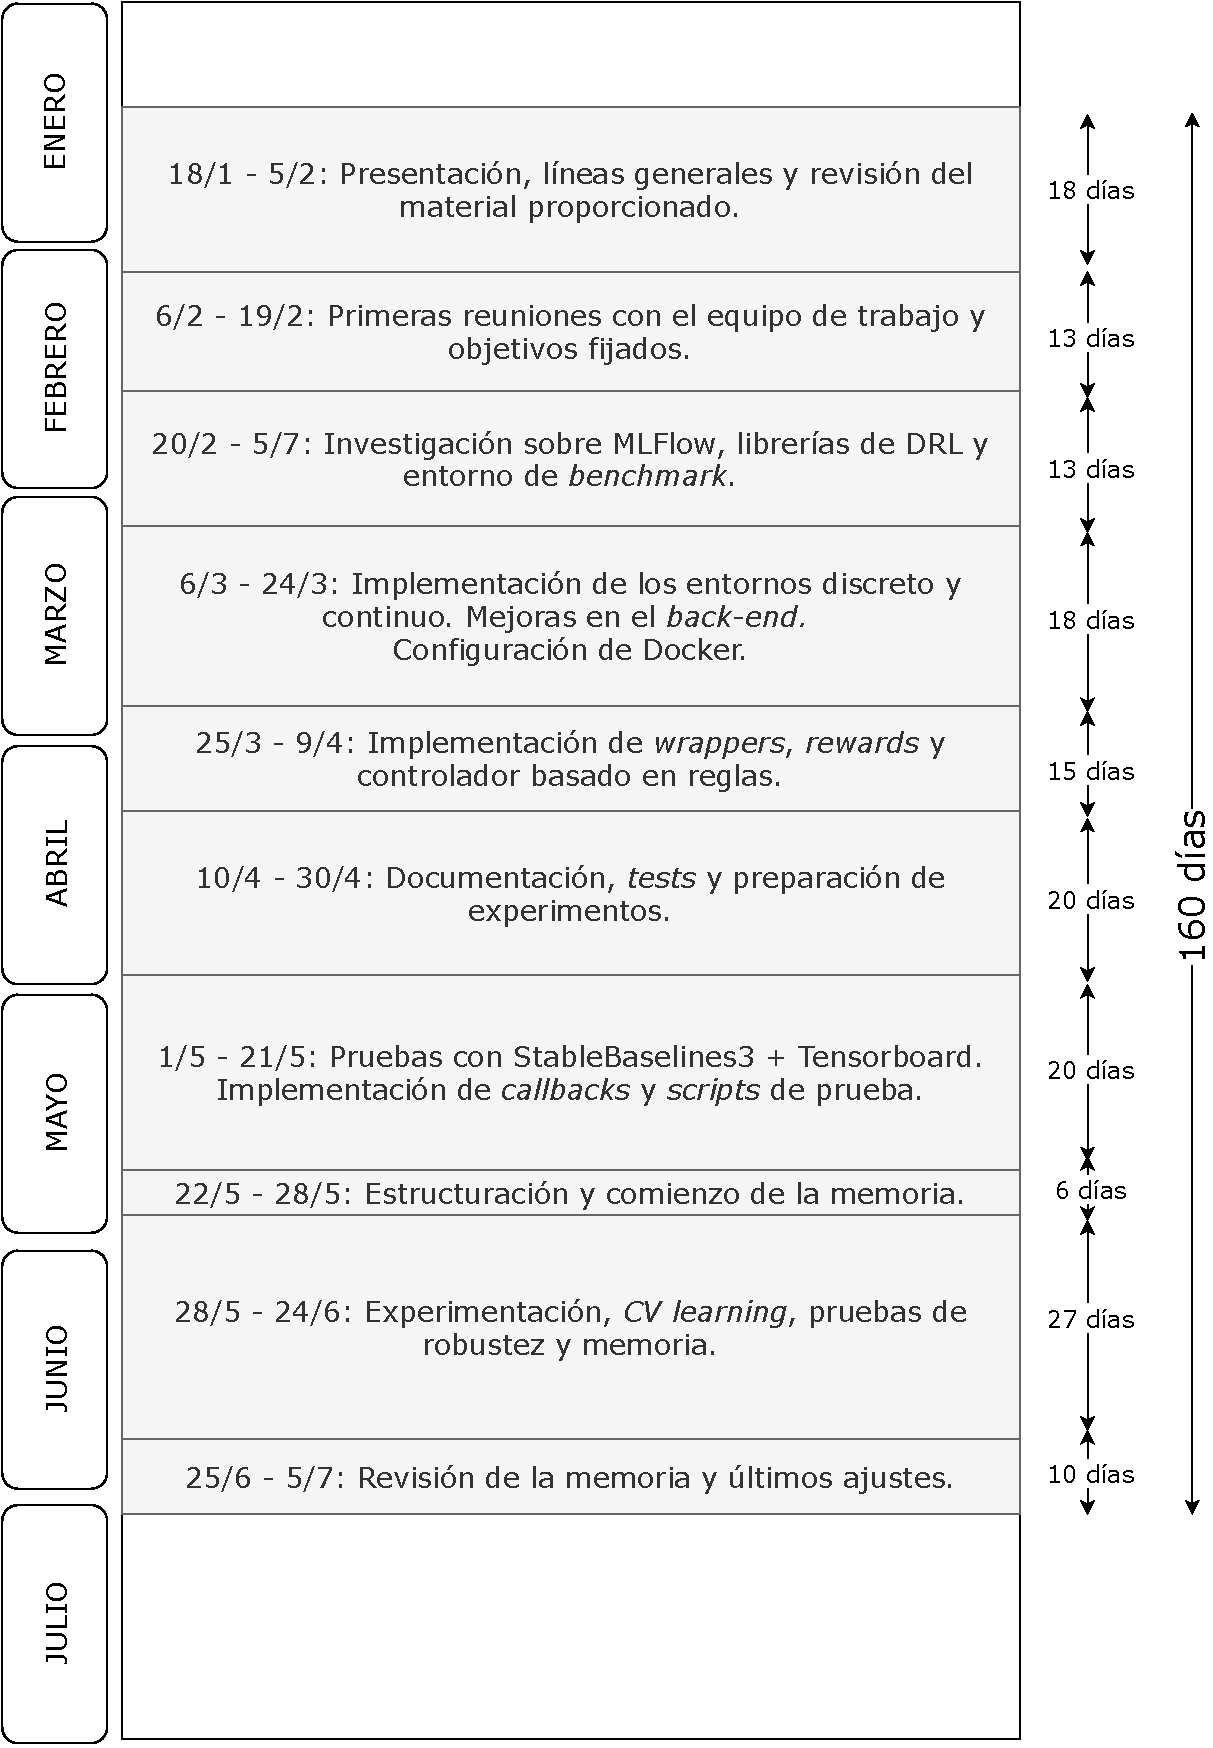
\includegraphics[width=\textwidth]{imagenes/planning.pdf}
    \caption{Planificación del proyecto}
    \label{fig:planning}
\end{figure}

Desde el punto de vista económico, los \textbf{gastos del proyecto} son los que se muestran en la Tabla \ref{tb:economico}. Algunos aspectos a considerar en su cálculo:

\begin{itemize}
    \item La estimación del coste por horas de trabajo se ha hecho de acuerdo a un salario medio aproximado de científico de datos de $25.000$ \euro\ según la plataforma \href{https://www.glassdoor.es/}{Glassdoor} a fecha de Junio de 2021.
    \item Los porcentajes de cotización a la seguridad social fueron obtenidos desde la web del \href{https://www.seg-social.es/wps/portal/wss/internet/Trabajadores/CotizacionRecaudacionTrabajadores/36537}{Ministerio de Inclusión, Seguridad Social y Migraciones} a fecha de Junio de 2021.
    \item El IRPF ha sido calculado mediante la herramienta online proporcionada por \href{https://cincodias.elpais.com/herramientas/calculadora-irpf/}{CincoDías} para un ingeniero de 23 años, con sueldo bruto anual de $25.000$ \euro.
    \item Por otro lado, en la estimación de costes indirectos se han tenido en cuenta el consumo eléctrico medio y el \textit{hardware} empleado.
\end{itemize}

Así, con una duración aproximada de 6 meses, el \textbf{coste total} del proyecto se estima en 2.574,00 $\times$ 6 $=$ 15.444,00 \euro.

\begin{table}
    \centering
    \caption{Desglose de gastos del proyecto}
    \label{tb:economico}
    \resizebox{\textwidth}{!}{%
    \begin{tabular}{|l|c|}
    \hline
    \textbf{Variable} & \textbf{Valor} \\ \hline
    Sueldo bruto anual (\euro) & 25.000 \\ \hline
    Número de pagas (\euro) & 6 \\ \hline
    Sueldo bruto mensual (\euro) & 2.083,33 \\ \hline
    Cotización a la seguridad social (\% empresa) & 23,60 \\ \hline
    Cotización a la seguridad social (\% trabajador) & 4,70 \\ \hline
    IRPF (\%) & 14,28 \\ \hline
    \textbf{Sueldo neto mensual del empleado} (\euro) & \textbf{1.687,91} \\ \hline
    \textbf{Coste mensual para la empresa} (\euro) & \textbf{2.574,00} \\ \hline
    \end{tabular}%
    }
\end{table}

\section{Estructura}

Una vez definidos los objetivos del proyecto, en el Capítulo \ref{ch:2} abordaremos los fundamentos del aprendizaje por refuerzo y sus aplicaciones en control HVAC según el estado del arte. Posteriormente, en el Capítulo \ref{ch:3} se definirá el entorno de simulación \textit{Energym}, así como las aportaciones realizadas al mismo a lo largo de este proyecto. En el Capítulo \ref{ch:4} se describirán los principales resultados obtenidos tras la experimentación con diferentes agentes y entornos. Finalmente, en el Capítulo \ref{ch:5} abordaremos las conclusiones, trabajo futuro y lecciones aprendidas tras el desarrollo de este proyecto.

Todo el código empleado y al que haremos referencia a lo largo de este documento puede encontrarse en el siguiente repositorio de GitHub: \url{https://github.com/manjavacas/drl-building}. También puede consultarse la documentación de la librería \textit{Energym} elaborada durante el desarrollo de este trabajo: \url{https://energym.readthedocs.io/}, así como su código fuente: \url{https://github.com/jajimer/energym}.



\chapter{Marco teórico}
\label{ch:2}

En este capítulo se ofrecerá un resumen del estado del arte en el ámbito del aprendizaje por refuerzo y aprendizaje profundo por refuerzo, dando a conocer las nociones básicas de los métodos que los comprenden, así como sus aplicaciones en el control eficiente de dispositivos HVAC.

\section{Aprendizaje por refuerzo}

El \textbf{aprendizaje por refuerzo} es un método de aprendizaje computacional centrado en la interacción de un agente con su entorno. Se trata de un aprendizaje iterativo, basado en prueba y error, donde el agente recibe recompensas positivas si sus acciones le conducen a estados deseables. El objetivo del agente será, por tanto, descubrir qué acciones le conducen a la maximización de dicha recompensa \cite{sutton2018reinforcement}.

Este modelo de aprendizaje está inspirado en la psicología conductista y el condicionamiento clásico, tratando de modelar el aprendizaje animal desde la perspectiva computacional del aprendizaje automático. Clásicamente, el campo del aprendizaje automático ha sido mayoritariamente definido como la unión de los paradigmas del \textit{aprendizaje supervisado} y \textit{no supervisado}. No obstante, si los comparamos con el \textit{aprendizaje por refuerzo}, encontramos aspectos significativos que permiten diferenciarlos:

\begin{itemize}
    \item En comparación con el \textbf{aprendizaje supervisado}, basado en el aprendizaje a partir de ejemplos previamente etiquetados por un supervisor externo, en el ámbito del \textit{aprendizaje por refuerzo} el agente debe ser capaz de aprender a partir de su propia experiencia. Esto hace que el \textit{aprendizaje supervisado} pierda valor en problemas donde el aprendizaje se produce en base a la interacción.
    \item Por otro lado, también existen diferencias con respecto al \textbf{aprendizaje no supervisado}, centrado en el descubrimiento de patrones en conjuntos de datos no etiquetados. Aunque tanto el \textit{aprendizaje no supervisado} como el \textit{aprendizaje por refuerzo} carecen de ejemplos de comportamiento ``correcto'', el \textit{aprendizaje por refuerzo} trata de maximizar una señal de recompensa, en lugar de intentar encontrar patrones ocultos en los datos.
\end{itemize}

Ante esta diferenciación, podemos considerar el \textit{aprendizaje por refuerzo} como un paradigma adicional dentro del aprendizaje automático.

\subsection{Conceptos básicos}

Tal y como se muestra en la Figura \ref{fig:rl-model}, un problema de \textit{aprendizaje por refuerzo} (en adelante, RL) queda definido por los siguientes componentes:

\begin{itemize}
    \item Un \textbf{agente} que aprende a partir de la interacción con su entorno y que persigue un determinado objetivo. Las interacciones entre el agente y el entorno se producen en una serie de \textbf{pasos} o \textit{timesteps}. En cada paso, el agente observa el \textit{entorno}, realiza una \textit{acción} y recibe una nueva \textit{observación} y \textit{recompensa}. Un \textbf{episodio} es una secuencia de \textit{pasos}, que parte de un \textbf{estado inicial} y termina en un \textbf{estado terminal}\footnote{En caso de encontrarnos ante un \textit{problema continuado}, como es el caso del problema tratado en este trabajo, no existe un estado terminal como tal. En estas situaciones es necesario establecer una limitación temporal o máximo número de \textit{pasos} que determine la finalización de los episodios.}.
    \item Un \textbf{entorno}, definido como todo elemento externo al agente. Se trata de un proceso dinámico que produce datos relevantes para el agente.
    \item Un conjunto de \textbf{estados} u \textbf{observaciones} que representan la situación actual del \textit{agente} en el \textit{entorno}. Dependiendo de si la percepción del \textit{entorno} por parte del agente es total o parcial, hablaremos de \textit{estados} u \textit{observaciones}, respectivamente. El espacio de estados puede ser finito o infinito, donde cada estado queda definido por un conjunto finito de variables.
    \item Una serie de \textbf{acciones} que determinan las dinámicas del \textit{entorno}. El \textit{agente} realiza \textit{acciones} sobre el \textit{entorno} que le permiten transitar entre diferentes \textit{estados}.
    \item Una función de \textbf{recompensa}. Se trata de un valor numérico que valora cómo de ``buena'' es una \textit{acción} o \textit{estado} para el \textit{agente}, por lo que puede corresponderse con una señal positiva (estado/acción deseable) o negativa (estado/acción a evitar). Uno de los principales retos del RL es conocer las consecuencias a largo plazo de las decisiones tomadas, cuya recompensa podría demorarse en el tiempo.
    \item Una \textbf{política} que determina, para cada \textit{estado}, la probabilidad de ejecutar cada una de las \textit{acciones disponibles}. Determina el comportamiento del agente y su preferencia ante diferentes estados o acciones.
\end{itemize}

\begin{figure}
    \centering
    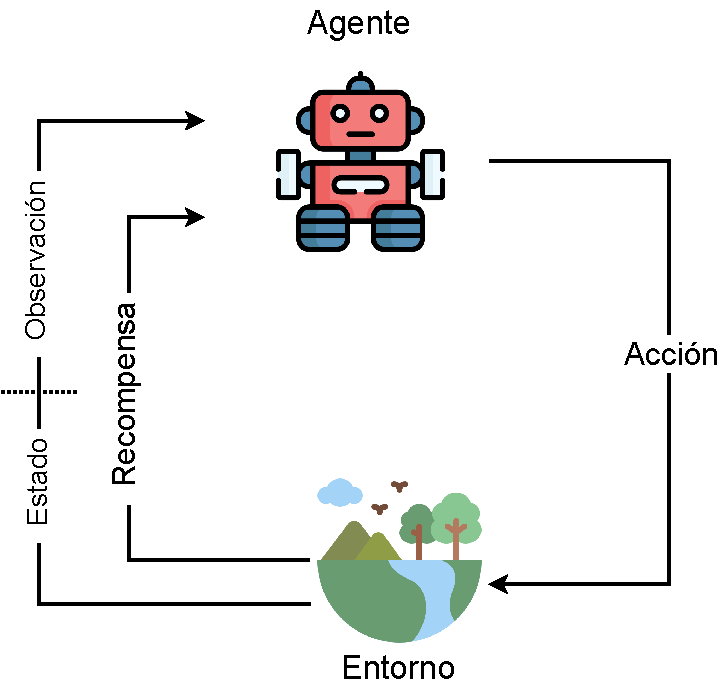
\includegraphics[width=0.6\textwidth]{imagenes/rl-components.pdf}
    \caption{Interacción \textit{agente}-\textit{entorno} en RL}
    \label{fig:rl-model}
\end{figure}

A diferencia de otros tipos de aprendizaje, a la hora de abordar un problema desde la perspectiva del RL es necesario establecer un equilibrio entre \textbf{exploración} y \textbf{explotación}. El agente debe \textit{explotar} las mejores acciones que ha encontrado hasta el momento para maximizar la recompensa obtenida, pero también debe estar abierto a \textit{explorar} alternativas que \textit{a priori} pueden resultar peores, pero que a largo plazo podrían conducir a mejores resultados.

\subsection{Procesos de decisión de Markov}

Formalmente, un problema de RL puede definirse como un \textbf{proceso de decisión de Markov} (MDP) compuesto por la quíntupla $(\mathcal{S}, \mathcal{A}, \mathcal{R}, \mathcal{P}, \gamma)$, donde:

\begin{itemize}
    \item $\mathcal{S}$ es el conjunto de todos los posibles \textit{estados};
    \item $\mathcal{A}$ el conjunto o espacio de \textit{acciones} disponibles;
    \item $\mathcal{R}$ es la función de \textit{recompensa};
    \item $\mathcal{P}$ son las \textit{probabilidades de transición} entre estados;
    \item $\gamma$ es un factor de descuento $\in [0, 1]$.
\end{itemize}

Los MDPs parten de la suposición de que las probabilidades de alcanzar un estado $s_t$ dado el estado $s_{t-1}$ y acción $a_{t-1}$ actuales son totalmente independientes de las interacciones previas. Es lo que conocemos como \textbf{Propiedad de Markov}, la cual se formula tal que:

\begin{equation}
    P(s'|s,a) \doteq P(s'|s, a, S_{t-1}, A_{t-1}, S_{t-2}, A_{t-2}, ...)
\end{equation}

Dicha propiedad nos permite definir una \textbf{función de transición} $\tau$ que devuelve el conjunto de probabilidades de transición asociadas a un estado y acción actuales. Esto es:

\begin{equation}
    \tau(s,a,s') \doteq p(s'|s,a) = P(S_t = s'|S_{t-1} = s, A_{t-1} = a)
\end{equation}

En problemas totalmente \textbf{determinísticos}, la función de transición devolverá un único estado con probabilidad 1 cuando se realice una acción desde un determinado estado. Por el contrario, en problemas \textbf{estocásticos} existen diferentes probabilidades de transición a nuevos estados, lo que supone cierta aleatoriedad en las dinámicas del entorno. En ambos casos se asume que la suma de las probabilidades siempre será 1:

\begin{equation}
    \sum p(s'|s,a) = 1
\end{equation}

Como ya hemos adelantado, las transiciones entre estados por parte del agente conducen a determinadas recompensas. Éstas vendrán definidas por una \textbf{función de recompensa}: una señal numérica que representa cómo de buena o mala es la transición a cierto estado desde la situación actual del agente.

Existen diferentes formas de representar la función de recompensa dependiendo de las variables involucradas en su cálculo: $\mathcal{R}(s)$, $\mathcal{R}(s,a)$ o $\mathcal{R}(s,a,s')$, siendo esta última la formulación más habitual, al ser más explícita y estar asociada a una menor pérdida de información \cite{morales2020grokking}.

Por tanto, la función de recompensa puede ser formulada tal que:

\begin{equation}
     r(s,a,s') \doteq \mathds{E}[R_t|S_{t-1} = s, A_{t-1} = a, S_t = s']
\end{equation}

El objetivo del agente será maximizar la \textbf{recompensa acumulada} (\textit{return}) desde el inicio de un episodio hasta su final. Siento $T$ el número total de \textit{pasos} de un \textit{episodio}, la recompensa acumulada se define como:

\begin{equation}
    G_t \doteq R_{t+1} + R_{t+2} + R_{t+3} + ... + R_T
\end{equation}

A la hora de estimar la recompensa acumulada, es común emplear un \textbf{factor de descuento}, $\gamma$, que ajusta la importancia de las recompensas a lo largo del tiempo. De esta forma, cuanto más tarde se reciba una recompensa, menor peso tendrá en el cálculo de la recompensa total esperada (ver Figura \ref{fig:discount}). Esto nos permite modelar la incertidumbre acerca de recompensas futuras, dando un mayor peso a recompensas inmediatas, o incluso ayudar a modelar problemas no episódicos donde la recompensa del futuro lejano tiende a 0. Así, si añadimos $\gamma$ al cálculo de la recompensa acumulada, tenemos:

\begin{equation}
    \begin{aligned}
        G_t \doteq & R_{t+1} + \gamma R_{t+2} + \gamma^2 R_{t+3} + ... + \gamma^{T-1} R_T \\ = &  \sum_{k=0}^{\infty}\gamma^k R_{t+k+1}
    \end{aligned}
\end{equation}

\begin{figure}
    \centering
    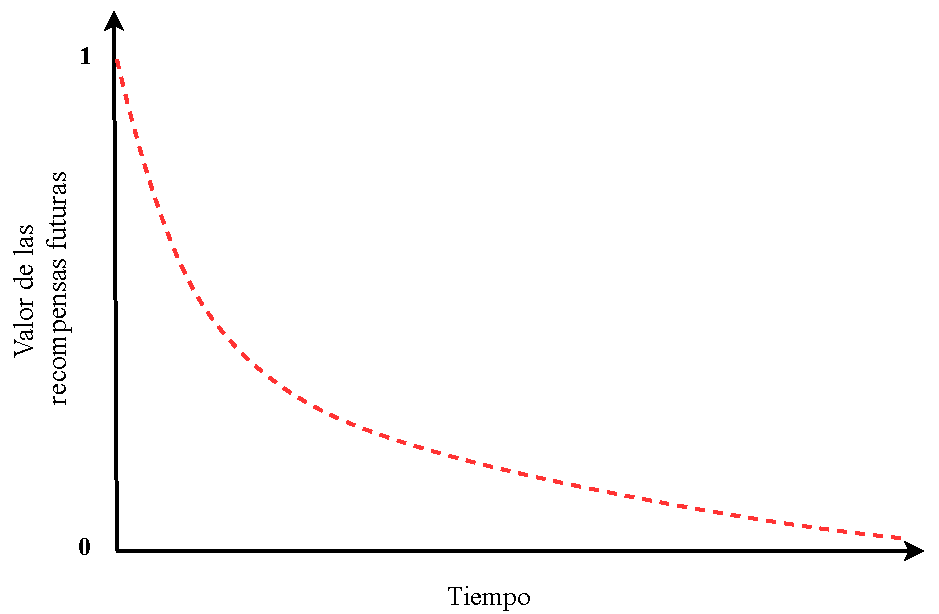
\includegraphics[width=0.9\textwidth]{imagenes/discount.pdf}
    \caption{Influencia del factor de descuento y el tiempo en el valor de las recompensas futuras}
    \label{fig:discount}
\end{figure}

Otra posible definición de la recompensa acumulada es la siguiente formulación recursiva:

\begin{equation}
    G_t \doteq R_{t+1} + \gamma G_{t+1}
\end{equation}

De esta forma, hemos definido los principales elementos que componen un MPD, contando con un modelo de entorno sobre el que un agente puede desenvolverse.

\subsection{Políticas y funciones de valor}

Una vez contamos con el modelo necesario para formular un problema de RL, es momento de abordar su resolución. Buscamos conocer la secuencia de acciones que maximice la recompensa acumulada al final de un episodio. Es aquí donde entra en juego el concepto de \textbf{política}, la cual, como ya adelantábamos, regirá el comportamiento del agente. 

Formalmente, una política es una función $\pi(a|s)$ que refleja la probabilidad de emplear una determinada acción $a \in \mathcal{A}(s)$ si el agente se encuentra actualmente en el estado $s \in \mathcal{S}$. En caso de tratarse de una política \textbf{determinista}, la acción devuelta por $\pi$ será siempre única ($probabilidad = 1$), mientras que, en caso de contar con una política \textbf{estocástica}, tendremos como salida la distribución de probabilidades de todas las acciones posibles.

Un ejemplo muy simple de política puede ser una \textit{función aleatoria}, la cual asigna la misma probabilidad a todas las acciones posibles partiendo del estado actual. Por lo general, una política aleatoria difícilmente permitirá maximizar la recompensa acumulada, al no verse guiada por los \textbf{objetivos} del agente. Un comportamiento más deseable sería, por ejemplo, asignar una mayor probabilidad a aquellas acciones que conduzcan a un estado más favorable y, por tanto, asociado a una mayor recompensa inmediata. Para lograrlo, será necesario definir una serie de funciones que permitan guiar al agente en la maximización de dicha recompensa. Definimos así las funciones \textit{estado-valor} y \textit{acción-valor}:

\begin{itemize}
    \item \textbf{Función estado-valor}, $v_\pi(s)$. Devuelve la recompensa esperada tras aplicar $\pi$ desde el estado $s$. Esto es:
    
    \begin{equation}
        v_\pi(s) \doteq \mathds{E}_\pi [G_t | S_t = s]
    \end{equation}
    
    Nótese cómo, de haberlo, el valor del estado terminal será siempre 0.
    
    \item \textbf{Función acción-valor}, $q_\pi(s,a)$. Devuelve la recompensa esperada tras aplicar la acción $a$ a partir de un estado $s$ siguiendo la política $\pi$. Se define tal que:
    
    \begin{equation}
        q_\pi(s,a) \doteq \mathds{E}_\pi [G_t | S_t = s, A_t = a]
    \end{equation}
\end{itemize}

Tanto $v_\pi$ como $q_\pi$ pueden estimarse a partir de la experiencia. Por ejemplo, un agente que sigue una política $\pi$ puede ir manteniendo la media de las recompensas obtenidas a partir de cada estado, de tal forma que $v_\pi(s)$ acabará convergiendo en el valor real de cada estado. Lo mismo ocurre para $q_\pi$ si se mantiene la recompensa media obtenida a partir de cada combinación estado-acción.

Visto en qué consiste la función \textit{estado-valor}, podemos desarrollarla recursivamente, dando lugar a la conocida como \textbf{ecuación de Bellman} \cite{bellman1966dynamic}:

\begin{equation}
    \begin{split}
        v_\pi(s) & \doteq \mathds{E}_\pi [G_t | S_t = s] \\
        & = \mathds{E}_\pi [R_{t+1} + \gamma G_{t+1} | S_t = s] \\ 
        &= \sum_{a} \pi(a|s) \sum_{s'}\sum_{r} p(s',r|s,a)[r + \gamma \mathds{E}_\pi [G_{t+1} | S_{t+1} = s']] \\ 
        & = \sum_{a} \pi(a|s) \sum_{s',r} p(s',r|s,a)[r + \gamma v_\pi(s')], \forall s \in \mathcal{S}
    \end{split}
\end{equation}

La ecuación de Bellman es un principio fundamental de la programación dinámica \cite{bellman1966dynamic} que expresa la relación entre el valor de un estado y el de sus sucesores. Concretamente, parte del promedio ponderado de todas las probabilidades de transición desde un estado inicial $s$, y establece que el valor de $s$ debe ser igual al valor descontado del siguiente estado esperado, más la recompensa esperada en el resto de la trayectoria a seguir.

El mismo principio puede aplicarse para la función \textit{acción-valor}, dando lugar a:

\begin{equation}
    \begin{split}
        q_\pi(s,a) & \doteq \mathds{E}_\pi [G_t | S_t = s, A_t = a] \\
        & = \mathds{E}_\pi [R_{t+1} + \gamma G_{t+1} | S_t = s, A_t = a] \\ 
        & = \sum_{s', r}p(s',r|s,a)[r + \gamma v_\pi(s')], \forall s \in \mathcal{S}, \forall a \in \mathcal{A}(s)
    \end{split}
\end{equation}

Una vez visto en qué consisten las políticas y funciones \textit{estado-valor} y \textit{acción-valor}, estas podrán servirnos para describir, evaluar y mejorar el comportamiento de los agentes. Como ya hemos indicado, el objetivo de un agente de RL es aspirar al \textbf{comportamiento óptimo} dentro de su entorno. Esta \textit{optimalidad} nos conduce a la definición de los siguientes términos:

\begin{itemize}
    \item \textbf{Política óptima}, $\pi_*$: aquella que, para cada estado, puede obtener recompensas esperadas mayores o iguales a las de cualquier otra política. Podemos comparar políticas en base a sus funciones \textit{estado-valor}:
    
        \begin{equation}
            \label{policy-comparison}
            \pi \geq \pi' \leftrightarrow v_\pi(s) \geq v_{\pi'}(s)
        \end{equation}
        
    De tal forma que la política óptima será aquella tal que:
    
        \begin{equation}
            \pi_* \geq \pi', \forall \pi'
        \end{equation}
   
    \item \textbf{Función \textit{estado-valor} óptima}, $v_*$: función \textit{estado-valor} que ofrece el máximo valor de todas las políticas para todos los estados.
    
        \begin{equation}
            v_*(s) = \underset{\pi}{max}\ v_\pi(s), \forall s \in S
        \end{equation}
    
    \item \textbf{Función \textit{acción-valor} óptima}, $q_*$: función \textit{acción-valor} que ofrece el máximo valor de todas las políticas para todo par \textit{estado-acción}.
    
        \begin{equation}
            q_*(s, a) = \underset{\pi}{max}\ q_\pi(s, a), \forall s \in S, \forall a \in \mathcal{A}(s)
        \end{equation}
\end{itemize}

Finalmente, cabe destacar que, mientras múltiples políticas óptimas pueden coexistir para un mismo MDP, únicamente existirá una única función \textit{estado-valor} y \textit{acción-valor} óptimas.

\subsection{Evaluación y mejora de las políticas}

Llegados a este punto, contamos con las herramientas necesarias para poder \textit{evaluar} políticas y funciones de valor, así como para calcular las funciones de valor y políticas óptimas.

El algoritmo de \textbf{evaluación iterativa de la política} (\textit{iterative policy evaluation}, o simplemente \textit{policy evaluation}) nos permite conocer cómo de ``buena'' o ``mala'' es una política cualquiera en base a su recompensa acumulada esperada. Este algoritmo (ver Algoritmo \ref{alg:policy-eval}, \cite{sutton2018reinforcement}) permite la aproximación iterativa de la función \textit{estado-valor} de la política evaluada a partir de la fórmula:

\begin{equation}
    v_{k+1}(s) =  \sum_{a} \pi(a|s) \sum_{s',r} p(s',r|s,a)[r + \gamma v_k(s')]
\end{equation}

\begin{algorithm}
\caption{Evaluación iterativa de la política}
\label{alg:policy-eval}
\DontPrintSemicolon
\LinesNumbered
\KwIn{$\pi$: la política a evaluar \newline
      $\mathcal{S}$: el espacio de estados del problema \newline
      $\gamma$: el factor de descuento \newline
      $\theta$: un umbral de convergencia}
\KwOut{$V$: los valores finales asociados a cada estado}

    $V(s) = 0, \forall s \in \mathcal{S}+$\;
    $V(terminal) = 0$\;
    
    \Repeat{$\Delta < \theta$}{
        $\Delta \leftarrow 0$\;
        \ForEach{$s \in \mathcal{S}$}{
            $v \leftarrow V(s)$\;
            $V(s) \leftarrow \sum_{a} \pi(a|s) \sum_{s',r} p(s',r|s,a)[r + \gamma V(s')]$\;
            $\Delta \leftarrow max(\Delta, |v-V(s)|)$\;
        }
    }
    
    \Return{V}

\end{algorithm}

donde los valores de los estados convergen cuando $k$ tiende a infinito. 

Una vez sabemos cómo \textit{evaluar} políticas, podemos compararlas entre sí, tal y como se mostró en \ref{policy-comparison}. De hecho, ahora somos capaces de partir de una política cualquiera y tratar de \textit{mejorarla} iterativamente a partir de la función \textit{acción-valor}. Para ello emplearemos el algoritmo de \textbf{mejora iterativa de la política} (ver Algoritmo \ref{alg:policy-impro}, \cite{sutton2018reinforcement}), el cual se define mediante la siguiente fórmula:

\begin{equation}
    \pi'(s) = \underset{a}{argmax}\ \sum_{s',r}p(s', r | s, a)[r + \gamma v_\pi(s')]
\end{equation}

Este algoritmo parte de la estimación de las recompensas para cada acción, $a$, desde el estado actual, $s$, y busca aquellas acciones que conducen al agente a estados sucesores, $s'$, con la máxima estimación \textit{estado-valor}.

\begin{algorithm}
\caption{Mejora iterativa de la política}
\label{alg:policy-impro}
\DontPrintSemicolon
\LinesNumbered
\KwIn{$\pi$: la política a evaluar \newline
      $\mathcal{S}$: el espacio de estados del problema \newline
      $\gamma$: el factor de descuento}
\KwOut{$V_*$: los valores finales asociados a cada estado \newline
       $\pi_*$: la política óptima obtenida}

    $politica\_estable \leftarrow verdadero$\;
    \ForEach{$s \in S$}{
        $a_0\leftarrow \pi(s)$\;
        $\pi(s) \leftarrow \underset{a}{argmax}\ \sum_{s',r}p(s', r | s, a)[r + \gamma V(s')]$\;
        \If{$a_0 \neq \pi(s)$}{
            $politica\_estable \leftarrow falso$\;
        }
    }
    \If{$politica\_estable$}{
        \Return{$V \approx v_*$ y $\pi \approx \pi_*$}\;
    }
    \Else{
        aplicar \textbf{evaluación de la política} y repetir\;
    }

\end{algorithm}

Si combinamos los procesos de evaluación y mejora de la política de forma cíclica, estaremos mejorando $\pi$ iterativamente. Es lo que se denomina \textbf{iteración de la política} (\textit{policy iteration}), consistente en alternar \textit{evaluación} y \textit{mejora} hasta converger en la política óptima ($\pi \approx \pi_*$).

Una solución alternativa a la iteración de la política es el algoritmo de \textbf{iteración de valor} (\textit{value iteration}), consistente en (ver Algoritmo \ref{alg:value-iter}):

\begin{enumerate}
    \item Encontrar la función \textit{estado-valor} óptima, $v_*$. El algoritmo parte de una función de valor aleatoria que mejora iterativamente hasta alcanzar su valor óptimo.
    \item Extraer la política óptima, $\pi_*$, asociada a $v_*$. Una vez contamos con la función de valor óptima, la política óptima $\pi_*$ será aquella que actúe de forma voraz con respecto a $v_*$.
\end{enumerate}

\begin{algorithm}
\caption{Iteración de valor}
\label{alg:value-iter}
\DontPrintSemicolon
\LinesNumbered
\KwIn{$\pi$: la política a evaluar \newline
      $\mathcal{S}$: el espacio de estados del problema \newline
      $\gamma$: el factor de descuento \newline
      $\theta$: un umbral de convergencia}
\KwOut{$V_*$: los valores finales asociados a cada estado \newline
       $\pi_*$: la política óptima obtenida}

    $V(s) = 0, \forall s \in \mathcal{S}+$\;
    $V(terminal) = 0$\;
    
    \Repeat{$\Delta < \theta$}{
        $\Delta \leftarrow 0$\;
        \ForEach{$s \in \mathcal{S}$}{
            $v \leftarrow V(s)$\;
            $V(s) \leftarrow \underset{a}{max}\ \sum_{s',r} p(s',r|s,a)[r + \gamma V(s')]$\;
            $\Delta \leftarrow max(\Delta, |v-V(s)|)$\;
        }
    }
    
    $\pi_*(s) \leftarrow \underset{a}{argmax} \sum_{s',r}p(s', r | s, a)[r + \gamma V(s')]$\;
    
    \Return{$V_*, \pi_*$}

\end{algorithm}

En la práctica, tal y como se indica en \cite{sutton2018reinforcement}, \textit{policy iteration} converge más rápido que \textit{value iteration} (ya que la política converge más rápido que la función \textit{estado-valor}); no obstante, es computacionalmente más complejo, ya que en cada iteración es necesario tanto evaluar como mejorar la política actual.

\subsection{Exploración y explotación}

Muchos de los problemas reales que podemos tratar de resolver mediante RL suponen espacios de estados y acciones muy grandes (o incluso infinitos). Esto hace que los métodos iterativos previamente mencionados sean inviables, ya que no serían capaces de estimar todos los valores y dar con una política óptima en un tiempo razonable. 

Como veremos más adelante, los métodos de aprendizaje utilizados para resolver este tipo de problemas deben dar cabida, no sólo a aprovechar el conocimiento del que ya dispone el agente tras haber interactuado con el entorno, sino también a tratar de conocerlo mejor a lo largo del tiempo.

Surge, pues, un nuevo problema hasta ahora no contemplado en la interacción del agente con el entorno: el balance entre \textbf{exploración} y \textbf{explotación}. Mientras que la \textit{exploración} hace referencia a transiciones entre estados no óptimas destinadas a conocer mejor el entorno, la \textit{explotación} tiene como fin maximizar la recompensa a partir del conocimiento sobre los estados y la política actual del agente.

Cuando un agente explora, ``sacrifica'' recompensas óptimas inmediatas en pos de descubrir nuevas trayectorias que puedan mejorar sus resultados futuros. No obstante, un agente que únicamente explora el entorno difícilmente convergerá en una buena solución, ya que nunca tomará las acciones que maximicen la recompensa. Es necesario, por tanto, buscar un equilibrio entre \textit{exploración} y \textit{explotación} que permita conocer el entorno de forma progresiva pero sin descuidar la acumulación de recompensas.

Existen diferentes formas de afrontar este equilibrio. Por ejemplo, el método $\epsilon$-\textit{greedy} se basa en actuar siguiendo una estrategia voraz (\textit{greedy}), pero permitiendo tomar acciones aleatorias bajo cierta probabilidad $\epsilon$. Dichas acciones aleatorias suponen \textit{explorar} en lugar de \textit{explotar}.

Finalmente, existen otras estrategias que consideran y/o codifican el factor de incertidumbre de los diferentes estados, de tal forma que, a medida que crece la incertidumbre sobre un estado, mayor probabilidad habrá de transitar hacia él.

\subsection{Algoritmos clásicos de RL}

Hasta el momento, hemos visto cómo emplear \textit{iteración de la política} e \textit{iteración de valor} para extraer la política óptima asociada a un MDP. Decimos, por tanto, que son \textbf{métodos dependientes del modelo} del entorno (\textit{model-based}). Concretamente, las funciones de transición y recompensa son las que definen las dinámicas del entorno, y las empleadas por estos métodos para optimizar la política empleada. Así, la principal ventaja de los métodos basados en modelos es que los estados futuros y las recompensas pueden anticiparse a través del modelo del entorno, lo que permite al agente a lograr una mejor planificación \cite{zhang2020taxonomy}.

No obstante, en la mayoría de problemas reales carecemos de un modelo que nos permita conocer de forma anticipada las dinámicas del entorno, ya sea por complejidad o por falta de información\footnote{Por ejemplo, podría darse el caso de que no se cumpliese la propiedad de Markov.}. Ante esta problemática, surgen los \textbf{métodos libres de modelo}, o \textit{model free}, los cuales estiman la función de valor y la política a partir de la experiencia. Estos modelos son más cercanos a la esencia de aprendizaje por refuerzo, ya que dependen exclusivamente del ensayo-error para aprender el comportamiento óptimo\footnote{Es lo que se denomina un \textit{problema de control}, en contraposición a los \textit{problemas de predicción} ya vistos, donde el objetivo era evaluar políticas o estimar funciones de valor dada una política. La resolución de un \textit{problema de control} consiste en optimizar de forma progresiva las estimaciones de la función \textit{acción-valor} \cite{morales2020grokking}.}. A continuación, estudiaremos en detalle su funcionamiento.

\subsubsection{Monte Carlo}

Los algoritmos de tipo \textbf{Monte Carlo} (MC) consisten en la ejecución de múltiples episodios que permitan recopilar diferentes trayectorias a lo largo del espacio de estados y acciones. De esta forma, el valor de cada estado será el promedio de las recompensas acumuladas en cada \textit{visita}. La misma filosofía puede aplicarse para estimar el valor de los pares estado-acción, especialmente si no disponemos de un modelo del entorno. Así, una vez conocido el valor de cada estado, o par acción-estado, podremos extraer la política óptima.

Nótese cómo, a medida que se simule un mayor número de episodios, el promedio de las recompensas para cada estado, $s$, tenderá a converger en $v_\pi(s)$. Lo mismo ocurrirá en el caso de los pares estado-acción, con tendencia a $q_\pi(s,a)$.

Uno de los problemas que pueden darse a la hora de calcular el promedio de las recompensas es que un estado (o par estado-acción) sea visitado múltiples veces en un mismo episodio. Ante esta situación, podemos considerar únicamente el valor obtenido en la primera visita (\textit{first-visit MC}; ver Algoritmo \ref{alg:first-MC}) o calcular la media de las recompensas obtenidas (\textit{every-visit MC}).

\begin{algorithm}
\caption{\textit{First-visit} MC, \cite{zhang2020taxonomy}}
\label{alg:first-MC}
\DontPrintSemicolon
\LinesNumbered
\KwIn{$\pi$: la política a evaluar}

Inicializar arbitrariamente $V(s), \forall s \in \mathcal{S}$\;
$recompensas(s) \leftarrow \{ \}, \forall s \in \mathcal{S}$\;

    \Repeat{no haya convergencia}{
        Generar un episodio siguiendo $\pi$: $S_0, A_0, R_1, S_1, A_1, R_2, ..., S_{T-1}, A_{T-1}, R_T$\;
        $G \leftarrow 0$\;
        $t \leftarrow T -1$\;
        \ForEach{paso en el episodio, $t = T - 1, T - 2, ... 0$}{
            $G \leftarrow \gamma G + R_{t+1}$\;
            \If{$S_0, S_1, ..., S_{t-1}$ no contiene a $S_t$}{
                $recompensas(S_t) \leftarrow recompensas(S_t) \cup \{G\}$
                $V(S_t) \leftarrow mean(recompensas(S_t))$\;
            }
        }
    }
\end{algorithm}

La exploración sigue siendo un factor importante, ya que adherirnos estrictamente a una política $\pi$ podría impedirnos conocer trayectorias que afecten a las estimaciones obtenidas. Es aconsejable, por tanto, seguir una política similar a $\epsilon$-\textit{greedy} que dé cabida a dicha exploración. De hecho, el valor de $\epsilon$ no tiene por qué ser estático, pudiendo ir reduciéndose a lo largo del tiempo, de tal forma que la exploración disminuya a medida que los valores estimados converjan \cite{morales2020grokking}.

Finalmente, aunque los algoritmos de tipo MC son sencillos y eficaces, también presentan ciertos problemas, tales como la necesidad de esperar a la finalización de cada episodio para actualizar los valores estimados, una alta variabilidad en las estimaciones, o tiempos de ejecución muy elevados para poder alcanzar la convergencia en entornos complejos.

\subsubsection{Diferencia temporal}

El aprendizaje por \textbf{diferencia temporal} (\textit{temporal-difference}, TD) es uno de los principales cimientos del aprendizaje por refuerzo, el cual combina ideas de los métodos basados en Monte Carlo y programación dinámica \cite{sutton2018reinforcement}. Además, constituye la base de algunos de los métodos que estudiaremos más adelante.

Tanto TD como Monte Carlo son métodos libres de modelo basados en la experiencia. En el caso de Monte Carlo, es necesario esperar a la finalización del episodio para calcular $V(S_t)$, ya que la estimación del valor de un estado depende de las estimaciones de todos los estados futuros visitados hasta obtener $G_t$. Veamos como representarlo formalmente:

\begin{itemize}
    \item Partimos de la idea de que la media $\mu_1, \mu_2, ..., \mu_n$ de una secuencia $x_1, x_2, ..., x_n$ puede calcularse de forma incremental de la siguiente forma:

    \begin{align}
        \mu_k = & \frac{1}{k} \sum_{j=1}^{k} x_j \\
              = & \frac{1}{k} (x_k + \sum_{j=1}^{k-1} x_j) \\
              = & \frac{1}{k} (x_k + (k-1)\mu_{k-1}) \\
              = & \mu_{k-1} + \frac{1}{k}(x_k - \mu_{k-1})
    \end{align}
    
    \item Cuando seguimos un método basado en MC, podemos aplicar esta idea para actualizar de forma incremental el valor de cada estado tras un episodio. De esta forma, para cada estado $S_t$, dada una recompensa final $G_t$:
    
    \begin{gather}
        N(S_t) \leftarrow N(S_t) + 1 \\
        V(S_t) \leftarrow V(S_t) + \frac{1}{N(S_t)}(G_t - V(S_t))
    \end{gather}
    
    O, de forma general:
    
    \begin{equation}
        V(s_{t+1}) \leftarrow V(s_t) + \alpha[objetivo - V(s_t)]
    \end{equation}
    
    siendo $\alpha$ un parámetro que representa el ``tamaño de paso'', o \textit{step-size}, y \textit{objetivo} la n-ésima recompensa obtenida\footnote{A la expresión $[objetivo - v(s_t)]$ se le denomina \textit{error de la estimación}, y se reduce conforme nos acercamos al \textit{objetivo}.}. 
    
    \item En el caso de MC, el objetivo es la recompensa final ($objetivo = G_t$). Esto, finalmente, nos lleva al cálculo incremental de $V(s_t)$:

    \begin{equation}
        V(S_t) \leftarrow V(S_t) + \alpha [G_t - V(S_t)]
    \end{equation}
    
    Podemos ver cómo los métodos basados en MC dependen de $G_t$ para actualizar el valor de los estados, lo que supone esperar a la finalización del episodio completo para actualizar dichas estimaciones.
\end{itemize}

A diferencia de Monte Carlo, TD no necesita esperar a conocer la recompensa final, $G_t$, para actualizar $V(s_t)$, sino únicamente esperar al siguiente \textit{paso}, $t+1$. Esto es:

\begin{equation}
    V(S_t) \leftarrow V(S_t) + \alpha[R_{t+1} + \gamma V(S_{t+1}) - V(S_t)]
\end{equation}

En este caso, $objetivo = R_{t+1} + \gamma V(S_{t+1})$, ya que se considera la recompensa $R_{t+1}$ y la estimación $V(S_{t+1})$ del siguiente \textit{timestep}\footnote{En este caso, $R_{t+1} + \gamma V(S_{t+1})$ es el \textit{objetivo} (\textit{TD target}), mientras que $R_{t+1} + \gamma V(S_{t+1}) - V(S_t)$ es el \textit{error} (TD error).}$^,$\footnote{Nótese cómo el valor de $\alpha$ pondera la importancia relativa de la nueva estimación de valor frente a la actual. Si $\alpha = 1$, se ignora la estimación previa, mientras que, si $\alpha = 0$, no se produce ninguna actualización.}. Es lo que denominamos $TD(0)$, o \textit{one-step TD} (ver Algoritmo \ref{alg:td}), el cual es un caso especial de \textit{n-step TD}:

\begin{equation}
    V_{t+n}(S_t) = V_{t+n-1}(S_t) + \alpha(G_{t:t+n} - V_{t+n-1}(S_t)
\end{equation}

Siendo $G_{t:t+n}$ la recompensa obtenida desde el instante $t$ hasta $t+n$; esto es: $R_{t+1} + \gamma R_{t+2} + ... + \gamma^{n-1} R_{t+n} + \gamma^n V_{t+n-1}(S_{t+n})$.

\begin{algorithm}
\caption{$TD(0)$, \cite{sutton2018reinforcement}}
\label{alg:td}
\DontPrintSemicolon
\LinesNumbered
\KwIn{$\pi$: la política a evaluar \newline
     $\alpha$: el \textit{step-size} $\in (0,1]$}

Inicializar arbitrariamente $V(s), \forall s \in \mathcal{S^+}$\;
$V(terminal) = 0$\;

 \ForEach{episodio}{
    Inicializar $S$\;
    \Repeat( para cada \textit{paso} en el episodio:){$S$ no sea terminal}{
        $A \leftarrow \pi(S)$\;
        Realizar acción $A$ y observar $R, S'$\;
        $V(S) \leftarrow V(S) + \alpha[R + \gamma V(S') - V(S)]$\;
        $S \leftarrow S'$\;
    }
 
 }
\end{algorithm}

En caso de utilizar \textit{n-step TD}, se nos plantea el interrogante de qué valor de $n$ utilizar. De hecho, podríamos plantear la posibilidad de combinar la información de múltiples \textit{timesteps} (por ejemplo, tomar como valores las medias de las estimaciones entre TD(2) y TD(4)) o incluso de todos ellos, asignando una mayor importancia a aquellos valores estimados más cercanos en el tiempo. Así surge el algoritmo $TD(\lambda)$, donde la recompensa $G^\lambda_t$ combina todas las recompensas en $G^{(n)}_t$, asignando una ponderación $(1-\lambda)\lambda^{n-1}$ a cada una de ellas. Esto es:

\begin{equation}
    G^\lambda_t = (1-\lambda) \sum^{\infty}_{n=1}\lambda^{n-1} G^{(n)}_t
\end{equation}

Así, $TD(\lambda)$ generaliza los métodos vistos hasta el momento, ya que equivale a Monte Carlo cuando $\lambda = 1$, y a $TD(0)$ cuando $\lambda = 0$. Existen, a su vez, dos formas de aplicar $TD(\lambda)$: hacia delante (\textit{forward-view}) o hacia atrás (\textit{backward-view}) \cite{morales2020grokking}:

\begin{itemize}
    \item \textit{Forward-view} $TD(\lambda)$: combina $n$ pasos en una sola actualización. El agente debe esperar hasta el final del episodio antes de poder actualizar las estimaciones.
    \item \textit{Backward-view} $TD(\lambda)$: divide las actualizaciones de los valores en actualizaciones parciales, que aplica en cada paso. Emplea rastros de elegibilidad (\textit{eligibility traces}) para decidir qué estados actualizar.
\end{itemize}

A modo de conclusión, TD es capaz de aprender a partir de episodios incompletos, actualizando estimaciones de valor en base a otras estimaciones de valor (es lo que se denomina \textit{bootstrapping}). Esto supone ciertas ventajas con respecto a MC, ya que:

\begin{itemize}
    \item TD puede aprender de forma \textit{online}, mientras que MC debe esperar al final del episodio hasta conocer la recompensa final obtenida.
    \item TD presenta una menor variabilidad en las estimaciones con respecto a MC.
    \item TD puede aprender a partir de secuencias incompletas, mientras que MC solamente aprende a partir de episodios completos.
    \item TD funciona en entornos continuados donde no existe un estado terminal, mientras que MC únicamente funciona en entornos episódicos.
\end{itemize}

Finalmente, cabe destacar cómo MC presenta un menor sesgo (\textit{bias}) en las estimaciones, ya que los valores se actualizan directamente en base a la recompensa final, y no con respecto a otras predicciones, como ocurre en el caso de TD.

\subsubsection{SARSA}

Una vez hemos visto como utilizar TD para resolver el problema de \textit{predicción}, estudiaremos cómo utilizarlo en \textit{control}. Partimos de la idea de que TD puede emplearse para calcular $q_\pi(s,a)$ de la misma forma que hicimos con $v_\pi(s,a)$:

\begin{equation}
    Q(S_t, A_t) \leftarrow Q(S_t, A_t) + \alpha \left [R_{t+1} + \gamma Q(S_{t+1}, A_{t+1}) - Q(S_t, A_t) \right ]
\end{equation}

Esta actualización se produce en cada transición desde estados no terminales $S_t$. Así, en caso de que $S_{t+1}$ sea terminal, $Q(S_{t+1}, A_{t+1}) = 0$. 

Podemos observar cómo el uso de cada uno de los elementos de la quíntupla $(S_t, A_t, R_{t+1}, S_{t+1}, A_{t+1})$ da lugar al nombre de este algoritmo: \textbf{SARSA} (ver Algoritmo \ref{alg:sarsa}).

\begin{algorithm}
\caption{SARSA (\textit{on-policy TD control)}, \cite{sutton2018reinforcement}}
\label{alg:sarsa}
\DontPrintSemicolon
\LinesNumbered
\KwIn{$\alpha$: el \textit{step-size} $\in (0,1]$ \newline
      $\epsilon > 0$}

Inicializar arbitrariamente $Q(s, a), \forall s \in \mathcal{S^+}, \ a \in \mathcal{A}(s)$\;
$Q(terminal, \cdot) = 0$\;

 \ForEach{episodio}{
    Inicializar $S$\;
    Elegir $A$ desde $S$ empleando una política derivada de $Q$ (por ejemplo, $\epsilon$-greedy)\;
    \Repeat( para cada \textit{paso} en el episodio:){$S$ no sea terminal}{
        Realizar acción $A$ y observar $R, S'$\;
        $Q(S,A) \leftarrow Q(S,A) + \alpha[R + \gamma Q(S',A') - Q(S,A)]$\;
        $S \leftarrow S'$; $A \leftarrow A'$\;
    }

 }
\end{algorithm}

Al igual que en el caso de TD, SARSA puede emplearse siguiendo un enfoque \textit{n-step}, dando lugar a \textit{n-step SARSA}, en contraposición a \textit{one-step SARSA} o \textit{SARSA(0)}. En este caso, la regla de actualización empleada es la siguiente:

\begin{equation}
    Q_{t+n}(S_t, A_t) = Q_{t+n-1}(S_t, A_t) + \alpha \left [G_{t:t+n} + \gamma Q_{t+n-1}(S_t, A_t) \right ]
\end{equation}

Llegados a este punto, es necesario diferenciar entre dos tipos de métodos: \textbf{on-policy} y \textbf{off-policy}:

\begin{itemize}
    \item Los métodos \textit{on-policy} estiman la recompensa $Q(s,a)$ asociada a cada par acción-estado asumiendo que se continuará siguiendo la política actual.
    \item Por otro lado, los métodos \textit{off-policy} actualizan el valor de cada par acción-estado asumiendo que posteriormente se seguirá una política voraz. De esta forma, la política actualizada es diferente a la que se asume que será seguida\footnote{Nótese cómo, en caso de seguir una política voraz, la distinción entre \textit{on-policy} y \textit{off-policy} desaparece.}.
\end{itemize}

Por tanto, decimos que SARSA es un método \textit{on-policy} porque la política que se utiliza para actualizar las estimaciones y la que se utiliza para actuar es la misma. 

\subsubsection{Q-learning}

Una alternativa \textit{off-policy} a SARSA es \textbf{Q-learning} \cite{watkins1992q}, un algoritmo de control de especial relevancia en el campo del aprendizaje por refuerzo. Decimos que Q-learning es un algoritmo \textit{off-policy} porque la política actualizada es diferente de la política de comportamiento:

\begin{itemize}
    \item La \textbf{política de comportamiento} (\textit{behavior policy}) se emplea para generar interacciones con el entorno.
    \item Por otro lado, la \textbf{política objetivo} (\textit{target policy}) es la política que el agente aprende.
\end{itemize}

La ecuación empleada por Q-learning para actualizar las estimaciones de cada par acción-estado es la siguiente (ver Algoritmo \ref{alg:qlearning}):

\begin{equation}
    Q(S_t, A_t) \leftarrow Q(S_t, A_t) + \alpha[R_{t+1} + \gamma\ \underset{a}{max}\ Q(S_{t+1}, a) - Q(S_t, A_t)]
\end{equation}

\begin{algorithm}
\caption{Q-learning (\textit{off-policy TD control)}, \cite{sutton2018reinforcement}}
\label{alg:qlearning}
\DontPrintSemicolon
\LinesNumbered
\KwIn{$\alpha$: el \textit{step-size} $\in (0,1]$ \newline
      $\epsilon > 0$}

Inicializar arbitrariamente $Q(s, a), \forall s \in \mathcal{S^+}, \ a \in \mathcal{A}(s)$\;
$Q(terminal, \cdot) = 0$\;

 \ForEach{episodio}{
    Inicializar $S$\;
    Elegir $A$ desde $S$ empleando una política derivada de $Q$ (por ejemplo, $\epsilon$-greedy)\;
    \Repeat( para cada \textit{paso} en el episodio:){$S$ no sea terminal}{
        Realizar acción $A$ y observar $R, S'$\;
        $Q(S, A) \leftarrow Q(S, A) + \alpha[R + \gamma\ \underset{a}{max}\ Q(S', a) - Q(S, A)]$\;
        $S \leftarrow S'$
    }

 }
\end{algorithm}

A diferencia de SARSA, Q-learning aprende una función acción-valor, $Q$, que se aproxima directamente a la función acción-valor óptima, $q_*$, independientemente de la política seguida. Así, Q-learning siempre convergerá en la política óptima.

Finalmente, desde un punto de vista computacional, lo habitual es representar los valores de cada par acción-estado a partir de una tabla $Q$ que se actualiza siguiendo el proceso mostrado en la Figura \ref{fig:qlearning}.

\begin{figure}
    \centering
    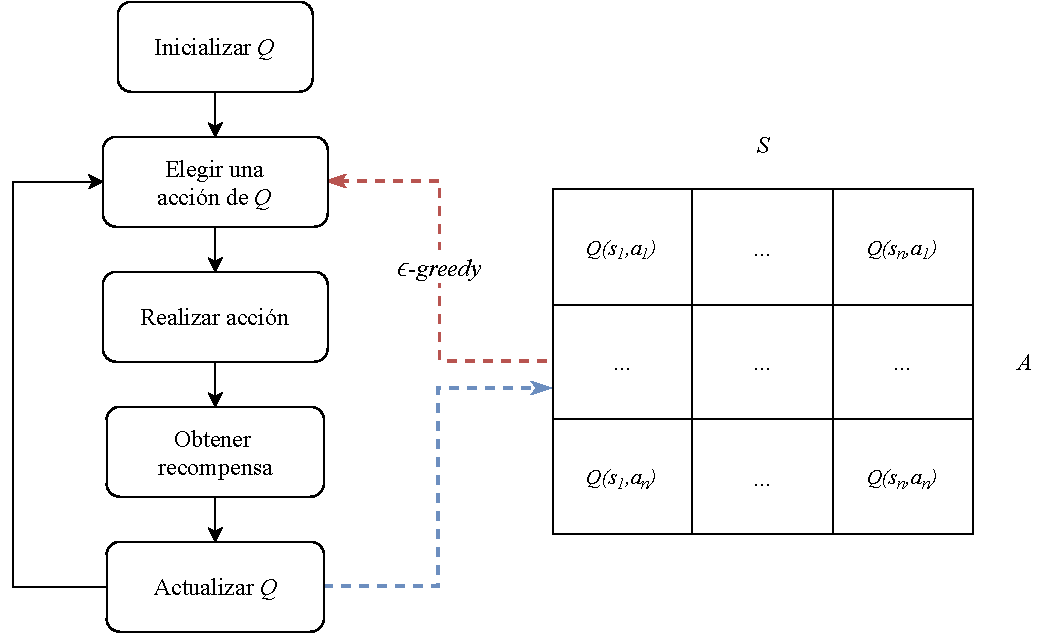
\includegraphics[width=\textwidth]{imagenes/qlearning.pdf}
    \caption{Entrenamiento mediante Q-learning}
    \label{fig:qlearning}
\end{figure}

\subsection{\textit{Deep Reinforcement Learning}}

Hasta el momento, hemos estudiado una serie algoritmos de RL ``clásicos'' capaces de ofrecer muy buenos resultados en entornos de baja complejidad. Simplemente actualizando de forma iterativa una tabla (\textit{lookup table} o \textit{memory table}) con diferentes estados, acciones y recompensas ha sido posible optimizar el comportamiento de un agente. No obstante, estos \textit{métodos tabulares} comienzan a ser inviables a medida que la complejidad de los entornos crece \cite{zai2020deep}. Dicho aumento en la complejidad puede venir dado por un considerable crecimiento en el número de acciones o estados que conforman el entorno, el cual puede tratar de paliarse con métodos \textit{ad hoc} difícilmente generalizables. Por ejemplo, un agente de RL que trabaja con imágenes podría adaptarse para únicamente atender a determinadas porciones de las mismas, en vez de utilizar todos los píxeles que las componen para definir un estado. De esta forma, estaríamos simplificando el espacio de estados, pero la solución propuesta podría no ser válida para otros problemas basados en imágenes donde las regiones a observar sean diferentes.

Ante este tipo de problemas, sería deseable contar con cierta capacidad de abstracción, permitiendo extraer la importancia de las diferentes características que definen un estado. Es aquí donde entra en juego el \textbf{aprendizaje profundo} (\textit{Deep Learning}, DL). En los últimos años, la combinación de RL con redes neuronales profundas ha dado lugar a lo que conocemos como \textbf{aprendizaje profundo por refuerzo} (\textit{Deep Reinforcement Learning}, DRL), el cual ha abierto la puerta a numerosas aplicaciones del aprendizaje por refuerzo en entornos reales. Así, los algoritmos de DRL combinan lo mejor de ambos mundos, dotando al aprendizaje por refuerzo de poder de representación, eficiencia y flexibilidad del aprendizaje profundo \cite{zai2020deep}.

En las siguientes subsecciones veremos algunos de los algoritmos de DRL más conocidos y empleados en este proyecto, abordando en detalle su funcionamiento y características.

\subsubsection{DQN}

Los algoritmos basados en \textbf{\textit{Deep Q-Networks}} (\textbf{DQN}) supusieron un importante hito en el ámbito del aprendizaje por refuerzo, siendo la primera aproximación a lo que hoy conocemos como DRL \cite{mnih2013playing, mnih2015human}. Se denominan métodos \textbf{basados en valor} (\textit{value-based)}, los cuales se fundamentan en el uso de redes neuronales para aproximar el valor de la función $Q$, que pasa a ser modelada de forma no lineal. De esta forma, sustituyen la tabla empleada por Q-learning por una red neuronal\footnote{Esta red puede ser un perceptrón multicapa (MLP) o, en el caso de trabajar con imágenes como datos de entrada, es común emplear redes neuronales convolucionales (CNN) como preprocesamiento previo al MLP. Un ejemplo muy representativo es el de los agentes entrenados para jugar a juegos de Atari \cite{mnih2013playing}.}, tal y como se muestra en la Figura \ref{fig:dqn}.

\begin{figure}
    \centering
    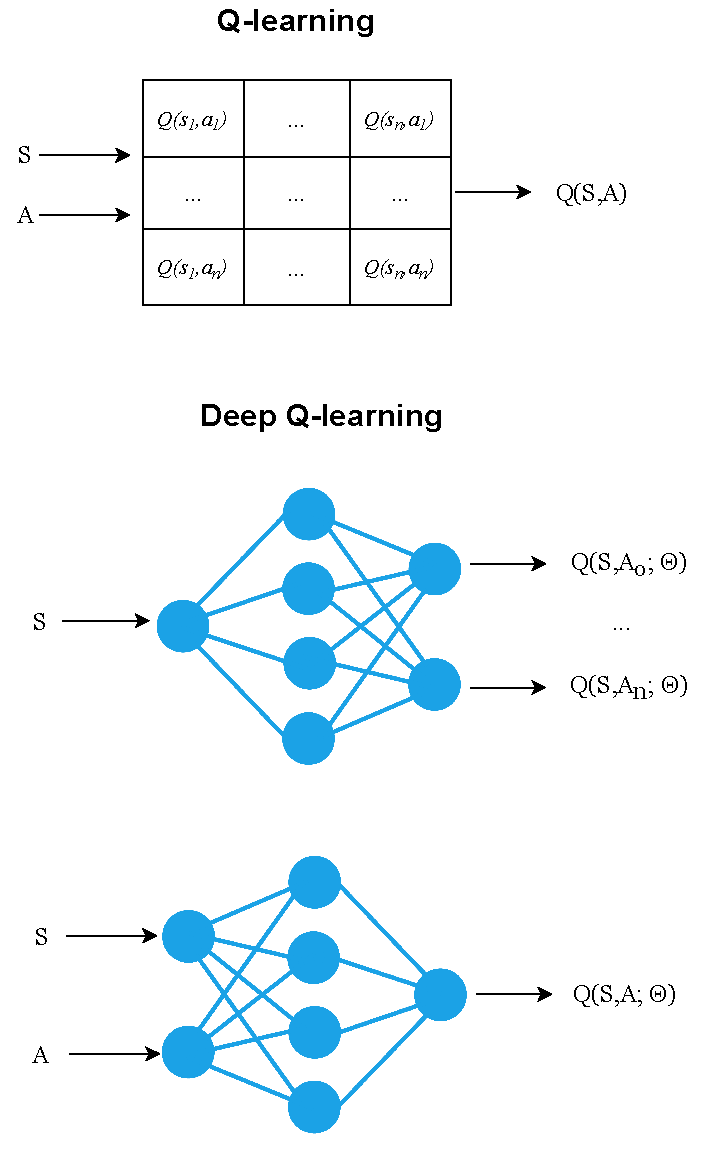
\includegraphics[width=0.7\textwidth]{imagenes/DQN.pdf}
    \caption{Diferencias entre Q-learning y DQN en sus diferentes formulaciones}
    \label{fig:dqn}
\end{figure}

Así, la capa de entrada de la red estará compuesta por tantas neuronas como variables conforman un estado u observación, mientras que las neuronas de salida serán tantas como acciones pueda realizar el agente. En base a la entrada $s$, la siguiente acción a realizar por el agente será la correspondiente a la neurona con mayor valor de salida en la \textit{Q-Network}: $Q(s,a_n;\theta)$, siendo $s$ el estado de entrada, $a_n$ la acción a realizar y $\theta$ el conjunto de pesos de la red\footnote{También es posible dar cabida a la exploración siguiendo una estrategia $\epsilon$-\textit{greedy}.}. Otras formulaciones alternativas permiten tomar pares estado-acción como entrada, para así obtener como salida el valor $Q(s,a; \theta)$ asociado a dicha entrada. Esta última formulación resulta de especial interés en problemas con espacios de acciones continuos, como se verá más adelante. 

Si atendemos a cómo estos sistemas aprenden, la función de pérdida (\textit{loss}) empleada por DQN es el error cuadrático medio (MSE) de la diferencia entre el $Q$-$value$ predicho y el valor objetivo, esto es:

\begin{equation}
    MSE = \mathds{E}_\pi[(Q(S,A) - Q(S,A;\theta))^2]
\end{equation}

Una de las principales limitaciones de DQN es el trabajo con espacios de acciones continuos, ya que al existir infinitas posibilidades no podremos obtener la acción óptima que sirva para computar el error. Dicho problema puede tratar de solventarse considerando como entrada el par $(s,a)$, o directamente discretizando el espacio de acciones, lo cual no deja de ser una limitación para este tipo de algoritmos. Esto lleva a que DQN, por lo general, no sea utilizado con espacios de acciones continuos.

El objetivo será, por tanto, medir la diferencia entre el valor real de $Q$ y el obtenido por la red, para finalmente aplicar descenso del gradiente y optimizar la función de error. La actualización de los pesos de la red se lleva a cabo de acuerdo a:
    
\begin{gather}
    \Delta \Theta = \Delta w = - \eta \frac{\partial E}{\partial w} \\
    \frac{\partial E}{\partial w} = 2(Q(S,A)-Q(S,A;\Theta)) \frac{\partial Q(S,A;\Theta)}{\partial w} \\
    \frac{\partial Q(S,A;\Theta)}{\partial w} = \nabla_\Theta Q(S,A;\Theta) \\
    \Delta \theta = -2 \eta (Q(S,A) - Q(S,A;\Theta)) \nabla_\Theta Q(S,A;\Theta)
\end{gather}

Al no conocer $Q(S,A)$, se aplica la expresión ya vista en Q-learning:

\begin{gather}
    Q(S_0,A_0) \leftarrow Q(S_0,A_0) + \alpha[R_1 + \gamma \ \underset{a \in A}{max} \ Q(S_1,a) - Q(S_0, A_0)] \\
    \Delta \Theta = \alpha [R + \gamma \ \underset{a \in A}{max} Q(S',a;\Theta)-Q(S,A;\Theta)] \nabla_\Theta \ Q(S,A;\Theta)
\end{gather}

Llegados a este punto, un problema que se nos plantea es que la misma red está calculando tanto el valor $Q$ predicho como el valor objetivo. Teniendo en cuenta esto, cuando los pesos se actualicen, los valores $Q$ de salida se actualizarán, pero también lo harán los valores $Q$ objetivo, ya que los objetivos se calculan utilizando los mismos pesos. Así, nuestros valores $Q$ se actualizarán con cada iteración para acercarse a los valores $Q$ objetivo, pero los valores $Q$ objetivo también se moverán en la misma dirección. 

Esto nos lleva a introducir una segunda red que haga el entrenamiento más estable, tal y como se propone en el artículo original \cite{mnih2015human} (ver Figura \ref{fig:dqn-nets}):

\begin{itemize}
    \item Por un lado, la \textbf{red de predicción} (\textit{prediction network}) es la encargada de calcular el valor $Q(S,A;\Theta)$.
    \item Por otro lado, la \textbf{red objetivo} (\textit{target network}) se encarga de estimar el valor objetivo, permitiendo el cálculo del error de forma imparcial. Se sincroniza con la red de predicción cada cierto número de iteraciones, lo que hace que sus pesos se actualicen con menor frecuencia.
\end{itemize}

\begin{figure}
    \centering
    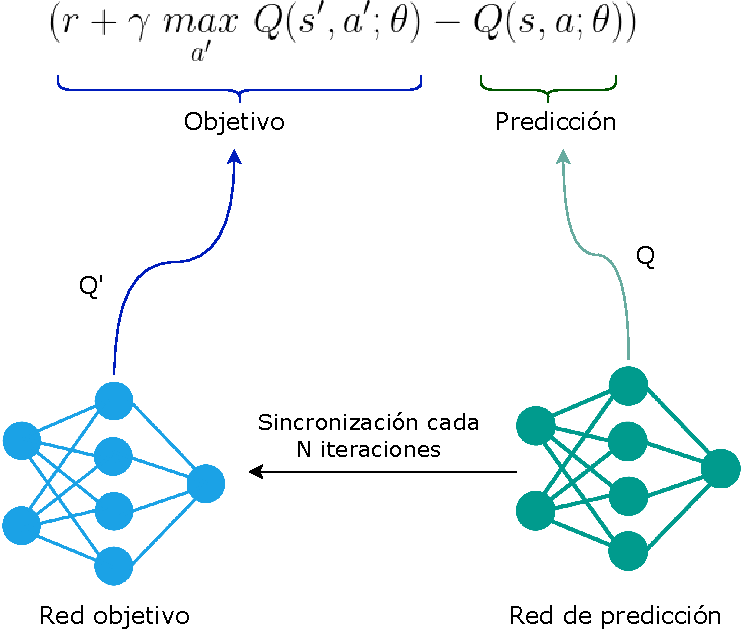
\includegraphics[width=0.8\textwidth]{imagenes/dqn-nets.pdf}
    \caption{Redes empleadas por DQN}
    \label{fig:dqn-nets}
\end{figure}

De forma adicional, es común combinar DQN con una \textbf{memoria de experiencias} que permita almacenar y utilizar como entrada diferentes muestras de experiencias pasadas $(S_t, A_t, R_t, S_{t+1})$ para predecir nuevos valores. Es lo que denominamos \textbf{repetición de la experiencia} \textit{experience replay}.

Finalmente, el proceso de aprendizaje mediante DQN queda resumido en el Algoritmo \ref{alg:dqn}. Cabe destacar la existencia de diferentes variantes de DQN orientadas a mejorar el método original, tales como \textit{Double Q-Learning} \cite{van2016deep}, \textit{Prioritized replay} \cite{schaul2015prioritized} o \textit{Dueling DQN} \cite{wang2016dueling}.

\begin{algorithm}
\caption{DQN}
\label{alg:dqn}
\DontPrintSemicolon
\LinesNumbered
\KwIn{$N$: número de iteraciones necesarias para sincronizar las redes de predicción y objetivo.}

    Inicializar la memoria de experiencias.\;
    Inicializar la red de predicción aleatoriamente.\;
    Crear la red objetivo como una copia de la red de predicción.\;

    $k \leftarrow 0$\;
    
    \ForEach{episodio}{
        
        Inicializar el estado inicial\;
        
        \ForEach{timestep}{
        
            $a \leftarrow$ seleccionar una acción (vía exploración o explotación) en base al valor de $Q$ predicho.\;
            Ejecutar la acción $a$, y observar la recompensa $r$ y el nuevo estado $s'$.\;
            Almacenar la tupla $(s,a,r,s')$ en la memoria de experiencias.\;
            Seleccionar un lote (\textit{batch}) aleatorio de la memoria de experiencias.\;
            Introducir \textit{batch} en la red de predicción\;
            Obtener la salida de la red objetivo para $s'$.\;
            Calcular el error (\textit{loss}) entre los valores $Q$ de salida y objetivo.\;
            Aplicar descenso del gradiente para actualizar los pesos de la red de predicción y reducir el valor de \textit{loss}.\;
            
            \If{$k = N$}{
                Actualizar pesos de la red objetivo con los valores de los pesos de la red de predicción.\;
            }
            
            $k \leftarrow k + 1$\;
        
        }
}

\end{algorithm}

\subsubsection{PPO}

Los métodos basados en \textbf{optimización de la política próxima} (\textit{Proximal Policy Optimization}, o \textbf{PPO}) \cite{schulman2017proximal, hsu2020revisiting} incorporan el gradiente de políticas al aprendizaje por refuerzo. Se trata de un algoritmo \textit{online}, por lo que no emplea una memoria de experiencias. El proceso de aprendizaje es el siguiente:

\begin{enumerate}
    \item Acumular experiencia hasta completar un lote o \textit{batch}.
    \item Utilizar dicha experiencia para optimizar la política.
    \item Descartar el \textit{batch} empleado y volver a 1.
\end{enumerate}

Al tratarse de un método \textit{online}, cada \textit{batch} solamente se emplea una vez para actualizar el gradiente, y después se desecha. Esto lleva a que los métodos basados en gradiente generalmente sean menos eficientes en el aprendizaje con respecto a métodos \textit{offline} como DQN.

Veamos en qué consiste este aprendizaje. PPO está basado en la \textbf{función de acción-ventaja}, la cual determina cómo de buena es una acción $a$ en base a la recompensa que normalmente se espera obtener siguiendo la política $\pi$:

\begin{equation}
\label{advantage}
    a_\pi(s,a) = q_\pi(s,a) - v_\pi(s)
\end{equation}

A partir de esta función acción-ventaja, definimos la función de pérdida como:

\begin{equation}
    L^{PG}(\theta) = \hat{\mathds{E}}_t[log\pi_\theta(a_t|s_t)\hat{A}_t]
\end{equation}

donde $\pi_\theta$ es la política seguida y $\hat{A}_t$ la función acción-ventaja. La idea será favorecer aquellas acciones que lleven a una función de ventaja positiva y, de esta forma, se incrementará la posibilidad de volver a elegir la acción $a$ a partir del estado $s$.

Uno de los principales problemas que supone esta forma de actualizar la política es que puede existir una alta divergencia entre la política original y la actualizada. Para evitar esto, PPO hace uso de \textbf{TRPO}  (\textit{Trust Region Policy Optimization}) y \textbf{KL} (coeficiente de divergencia de Kullback-Leibler) para establecer restricciones de divergencia que permitan que las actualizaciones se realicen únicamente dentro de una ``región de confianza'' \cite{schulman2015trust}. Esto permite que la nueva política obtenida no varíe demasiado con respecto a la anterior. Así, el siguiente ratio:

\begin{equation}
    r(\theta) = \frac{\pi_{\theta_ {old}}(a|s)}{\pi_\theta(a|s)}
\end{equation}

es empleado en la función objetivo de TRPO tal que:

\begin{equation}
    J(\theta)^{TRPO} = E[r(\theta) \hat{A}_{\theta_{old}}(s,a)]
\end{equation}

Si añadimos la restricción que obliga a que este ratio esté entre $1-\epsilon$ y $1+\epsilon$, tenemos la función objetivo empleada por PPO para actualizar la política:

\begin{equation}
    J^{CLIP}(\theta) = \mathds{E}[min(r(\theta)\hat{A}_{\theta_{old}}(s,a), clip(r(\theta), 1-\epsilon, 1+\epsilon)\hat{A}_{\theta_{old}}(s,a)]
\end{equation}

De esta forma, el ratio queda truncado en el rango $[1-\epsilon, 1+\epsilon]$ (mediante la función $clip$), evitando que se produzcan grandes desviaciones en la política, y de tal forma que PPO toma el valor mínimo entre el valor original y el truncado.

\subsubsection{A2C}

El algoritmo \textbf{\textit{Advantage Actor Critic}} (\textbf{A2C}) se encuentra dentro de la familia de métodos \textit{actor-critic} (ver Figura \ref{fig:actor-critic}) en los que una red \textit{actor} se encarga de aprender una política, mientras que otra red  \textit{crítica} se encarga de evaluarla. De esta forma, la red \textit{critic} aprende el valor de los estados, mapeando cada uno con su valor correspondiente. Esta información es empleada por la red \textit{actor} para mejorar el comportamiento, mapeando cada estado con una distribución de probabilidades que indican la preferencia por unas acciones u otras.

\begin{figure}
    \centering
    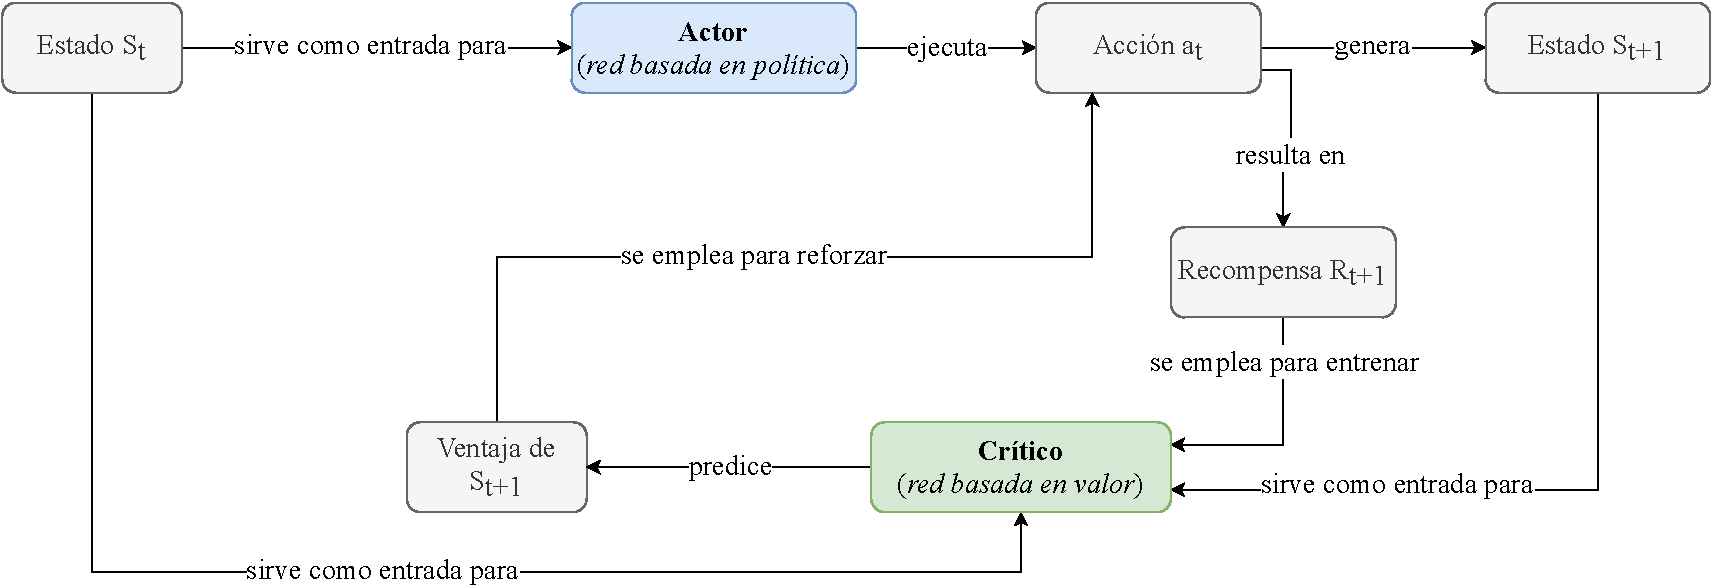
\includegraphics[width=\textwidth]{imagenes/actor-critic.pdf}
    \caption{Funcionamiento de modelos \textit{actor-critic}. Adaptado de \cite{zai2020deep}}
    \label{fig:actor-critic}
\end{figure}

A2C es una versión síncrona de \textbf{A3C} (\textit{Asynchronous Advantage Actor Critic}) \cite{mnih2016asynchronous}. Ambos están basados en la interacción entre diferentes nodos (\textit{\textbf{workers}}) encargados de generar experiencias a partir de una copia propia de la función de valor, la política y el entorno, tal y como se muestra en la Figura \ref{fig:a3c}. Así, en el caso de A3C, tras la recolección de un lote (\textit{batch}) de experiencias, cada \textit{worker} actualiza un \textbf{modelo global} de forma asíncrona, sin existir coordinación alguna con el resto de nodos. Posteriormente, los \textit{workers} actualizan su copia de los modelos y continúan el proceso de aprendizaje.

\begin{figure}
    \centering
    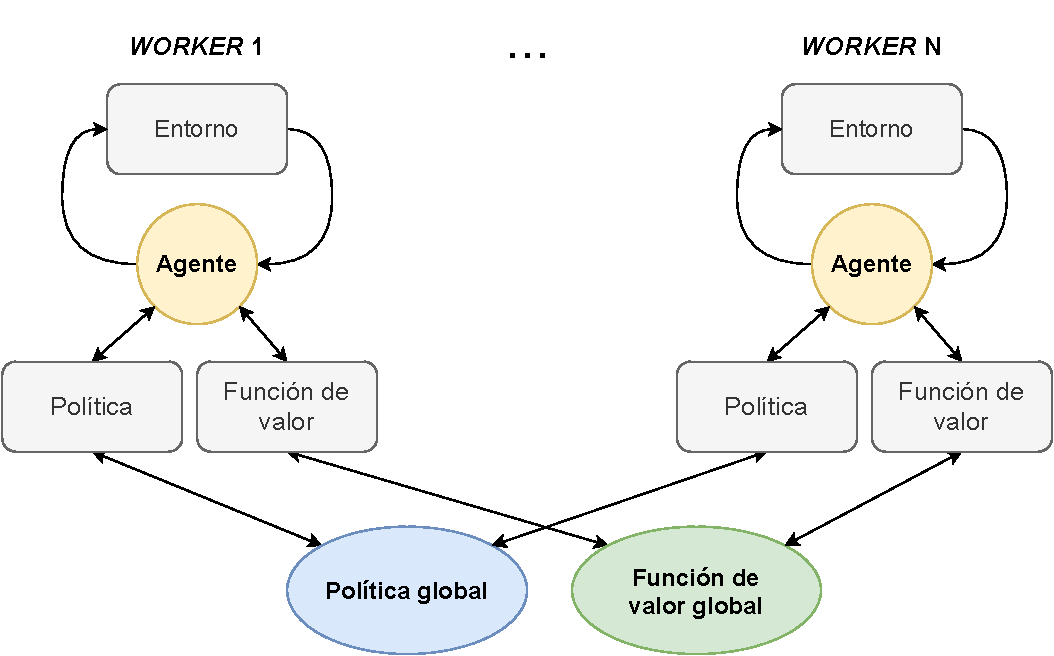
\includegraphics[width=\textwidth]{imagenes/A3C.pdf}
    \caption{Modelo A3C. Adaptado de \cite{morales2020grokking}}
    \label{fig:a3c}
\end{figure}

Por el contrario, A2C es una versión síncrona de A3C que cuenta con un único agente coordinando la interacción con el entorno, tal y como se muestra en la Figura \ref{fig:a2c}. De esta forma, en vez de tener múltiples nodos que actúan y aprenden, pasamos a contar con un único nodo aprendiendo a partir de la experiencia de diferentes actores.

\begin{figure}
    \centering
    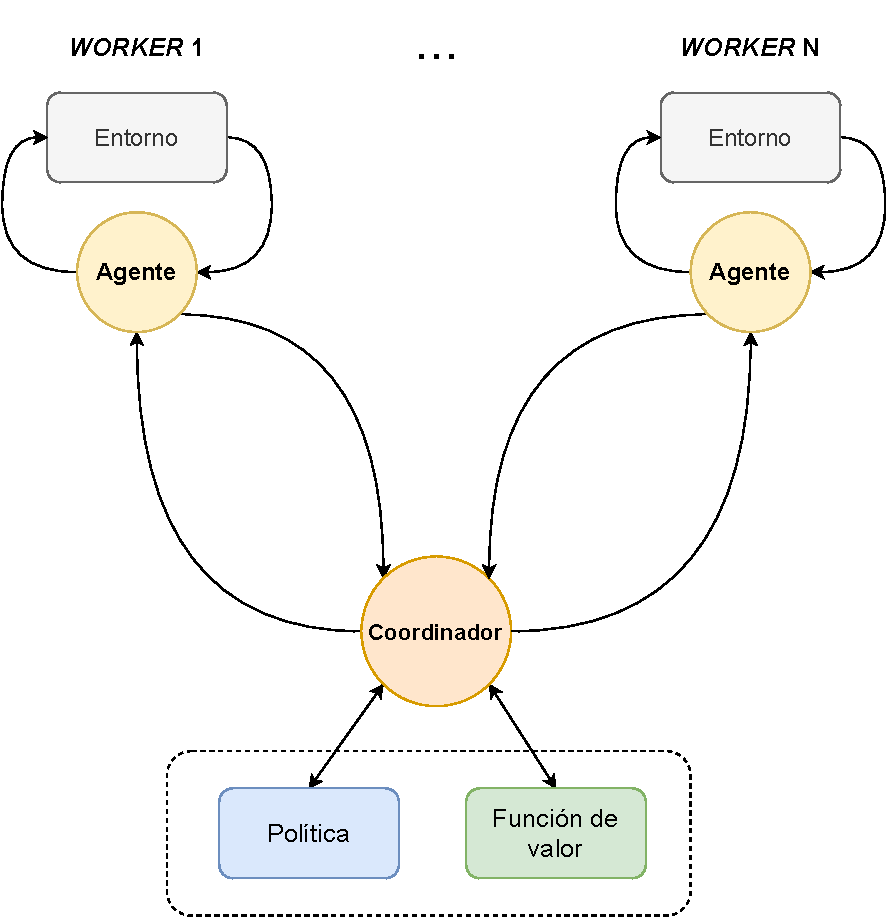
\includegraphics[width=0.7\textwidth]{imagenes/A2C.pdf}
    \caption{Modelo A2C}
    \label{fig:a2c}
\end{figure}

Así, en A2C el nodo \textbf{coordinador} espera a que todos los \textit{workers} terminen su trabajo antes de actualizar los parámetros globales. De esta forma, se consigue que en la siguiente iteración todos los \textit{workers} partan de la misma política. La actualización sincronizada del gradiente permite un entrenamiento más cohesionado, evitando que haya agentes empleando diferentes versiones de la política y logrando que la convergencia sea más rápida con respecto a A3C\footnote{Se ha demostrado que A2C es capaz de hacer un uso más eficiente de las GPUs, así como trabajar mejor con \textit{batches} de gran tamaño. De esta forma, A2C consigue un rendimiento igual o superior al de A3C (\url{https://openai.com/blog/baselines-acktr-a2c/).}}.

Finalmente, al tratarse de un método \textit{on-policy}, se sigue un proceso de aprendizaje similar al de PPO. Además, la función de ventaja previamente definida en la ecuación \ref{advantage} vuelve a ser un factor clave para computar el error y actualizar los pesos. Esta puede aproximarse mediante Monte Carlo (\ref{AdvMC}), empleando el ya conocido $TD$-$error$ ($R_{t+1} + \gamma V(S_{t+1}) - V(S_t)$) (\ref{AdvTD}) o a partir de una estimación \textit{n-step} (\ref{AdvNstep}):

\begin{align}
    A_\varphi(s_t,a_t) \approx\ & R(s_t, a_t) - V_\varphi(s_t) \label{AdvMC} \\
                       \approx\ & r(s_t,a_t,s_{t+1}) + \gamma V_\varphi(s_{t+1}) - V_\varphi(s_t) \label{AdvTD} \\
                       \approx\ & \sum_{k=0}^{n-1}\gamma^k r_{t+k+1} + \gamma^n V_\varphi(s_{t+n+1}) - V_\varphi(s_t) \label{AdvNstep}
\end{align}

A partir de esta función de ventaja, se lleva cabo la actualización de la red \textit{actor} tal que:

\begin{equation}
    \nabla_\theta J(\theta) = \sum_t \nabla_\theta\ log\ \pi_\theta(s_t,a_t) A_\varphi(s_t,a_t)
\end{equation}

Finalmente, el \textit{crítico} se actualiza tratando de minimizar el error $TD$ entre el valor estimado de un estado y su valor real:

    \begin{equation}
            \mathcal{L}(\varphi) = \sum_t A_\varphi(s_t,a_t)^2
    \end{equation}

\subsubsection{DDPG}

\textbf{\textit{Deep Deterministic Policy Gradient}} (\textbf{DDPG}) \cite{lillicrap2015continuous} es un algoritmo \textit{off-policy} de tipo \textit{actor-critic} basado en la combinación de \textbf{DPG} (\textit{Deterministic Policy Gradient}) \cite{silver2014deterministic} con \textbf{DQN}. Puede verse como una versión de DQN adaptada a entornos continuos \cite{zai2020deep}.

Hasta el momento hemos visto agentes que, al seguir una política estocástica $\pi_\theta(s)$, asignan cierta probabilidad a cada una de las acciones disponibles desde un estado $s$. Esto garantiza la exploración en ciertas ocasiones, ya que raramente una acción tendrá una probabilidad nula de ser seleccionada. Así, los métodos basados en valor como DQN tienen como fin converger en una política determinista que actúe de forma voraz tal que: $a_t^* = \underset{a}{argmax}\ Q_\theta(s_t,a)$. La exploración, como ya hemos mencionado, se asegura por medio de una política de comportamiento estocástico, como $\epsilon$-$greedy$, dando lugar a un aprendizaje \textit{off-policy}. 

DDPG, por el contrario, tiene como objetivo entrenar una \textbf{política determinista} parametrizada $\mu_\theta(s)$. Atendiendo al teorema del gradiente de la política \cite{sutton1999policy} tenemos:

\begin{equation}
    J(\theta) = \mathds{E}_{s\sim \rho_\mu}[R(s, \mu_\theta(s))]
\end{equation}

Así, en vez de tratar de maximizar el valor de la función $Q$ en el siguiente estado para obtener la acción voraz correspondiente (como ocurre en DQN), DDPG trata de aproximar la mejor acción en el siguiente estado utilizando una función de política $\mu$ \cite{morales2020grokking}. Por tanto, en comparación con la función de pérdida de DQN:

\begin{align}
    \mathcal{L}_i(\theta_i) = & \mathds{E}_{(s,a,r,s')\sim \mathcal{U}(\mathcal{D})} [(r+\gamma \underset{a'}{max}\ Q(s',a';\theta^-) - Q(s,a;\theta_i))^2] \\
    = & \mathds{E}_{(s,a,r,s')\sim \mathcal{U}(\mathcal{D})}[(r+\gamma Q(s', \underset{a'}{argmax}\ Q(s',a';\theta^-);\theta^-) - Q(s,a;\theta_i))^2]
\end{align}

la ecuación empleada por DDPG para computar el valor de pérdida es la siguiente:

\begin{equation}
    \mathcal{L}_i(\theta_i) = \mathds{E}_{(s,a,r,s')\sim \mathcal{U}(\mathcal{D})}[(r+\gamma Q(s', \mu(s';\phi^-);\theta^-) - Q(s,a;\theta_i))^2]
\end{equation}

En esta expresión podemos ver cómo $\mu$ aprende las acciones voraces determinísticas, a la vez que $\phi$ actúa como red objetivo. Podemos, por tanto, expresar la función objetivo de DDPG como:

\begin{equation}
    J_i(\phi_i) = \mathds{E}_{s\sim \mathcal{U}(\mathcal{D})}[Q(s,\mu(s;\phi);\theta]
\end{equation}

Una vez contamos con un método para entrenar políticas voraces deterministas, el problema que surge es cómo garantizar la exploración en el entrenamiento, ya que si la política no está entrenada, las acciones estrictamente voraces no son suficientes para obtener un comportamiento óptimo. 

Como tantas veces hemos mencionado, es necesario equilibrar exploración con explotación; sin embargo, DDPG aprende una política determinista, por lo que no explorará de forma \textit{on-policy}. Para dar solución a este problema, DDPG añade \textbf{ruido} (gaussiano) a las acciones seleccionadas por la política:

\begin{equation}
    \mu'(s) = \mu_\theta(s) + \mathcal{N}
\end{equation}

De esta forma, DDPG es capaz de extender DQN a entornos continuos siguiendo un enfoque \textit{actor-critic} y aprendiendo una política determinista óptima.

\subsubsection{SAC}

El último algoritmo de DRL empleado en este proyecto es \textbf{\textit{Soft Actor Critic}} (\textbf{SAC}) \cite{haarnoja2018soft}. Se trata de un método \textit{off-policy} de tipo \textit{actor-critic} que permite optimizar una política estocástica (a diferencia de DDPG) en entornos continuos.

Los métodos \textit{on-policy} como PPO o A3C son ineficientes en su aprendizaje debido a que necesitan información completamente nueva después de cada actualización de la política. Una alternativa más eficiente son los métodos \textit{off-policy} basados en Q-learning, como DDPG. Estos cuentan con un mejor rendimiento en el aprendizaje, ya que pueden aprender de forma eficiente a partir de información pasada almacenada en memoria (\textit{experience replay buffer}). Sin embargo, un inconveniente de este tipo de métodos es que son muy sensibles a los hiperparámetros de los que dependen, lo que dificulta su convergencia. SAC orienta sus esfuerzos en facilitar dicha convergencia.

Una característica fundamental de SAC es la \textbf{regularización de la entropía}. La política se entrena para maximizar un equilibrio entre la recompensa esperada y la entropía, la cual actúa como medida de aleatoriedad en el comportamiento del agente. Esto está estrechamente relacionado con el equilibrio entre exploración y explotación: aumentar la entropía da lugar a una mayor exploración, lo que puede acelerar el aprendizaje a largo plazo. También puede evitar que la política converja prematuramente en un óptimo local. 

Así, SAC supera el problema de la convergencia alentando a la política a explorar, evitando asignar una probabilidad muy alta a cualquier acción específica de las posibles. Si añadimos la mencionada entropía a la función objetivo del algoritmo, tenemos:

\begin{equation}
    J(\theta) = \sum_{t=1}^{T} \mathds{E}_{(s_t,a_t) \sim \rho_{\pi_\theta}}[r(s_t,a_t) + \alpha \mathcal{H}(\pi_\theta(\cdot|s_t))]
\end{equation}

donde $\mathcal{H}$ es la medida de entropía y $\alpha$ es un coeficiente que controla la importancia que se otorga a dicha medida\footnote{Este coeficiente $\alpha$ se denomina \textit{temperatura}. Su ajuste no es una tarea trivial, lo que ha llevado al desarrollo de nuevas versiones de SAC orientadas ajustar automáticamente su valor \cite{haarnoja2018soft}.}.

SAC hace uso de tres redes para realizar esta tarea de optimización\footnote{Ecuaciones extraídas de: \url{https://julien-vitay.net/deeprl/}.}:

\begin{enumerate}
    \item Una primera red encargada de aproximar la función de valor $V_\varphi$ (\textit{soft state-value function}) con la siguiente función de pérdida y actualización:
    
        \begin{equation}
            \mathcal{L}(\varphi) = \mathds{E}_{s_t \in \mathcal{D}} [\mathds{E}_{a_{t} \in \pi} [(Q_\psi(s_{t}, a_{t}) - \log \, \pi_\theta(s_t, a_t)] - V_\varphi(s_t) )^2]
        \end{equation}
    
        \begin{equation}
            \nabla_\varphi \mathcal{L}(\varphi) = \nabla_\varphi V_\varphi(s_t) \, (V_\varphi(s_t) - Q_\psi(s_{t}, a) + \log \, \pi_\theta(s_t, a) )
        \end{equation}
    
    \item Otra red encargada de estimar el valor de la función $Q_\psi$ (\textit{soft Q-value function}). Sus funciones de pérdida y actualización son:
    
        \begin{equation}
            \mathcal{L}(\psi) = \mathds{E}_{s_t, a_t \in \mathcal{D}} [(r_{t+1} + \gamma \, V_\varphi(s_{t+1}) - Q_\psi(s_t, a_t))^2]
        \end{equation}
        
        \begin{equation}
            \nabla_\psi \mathcal{L}(\psi) = - \nabla_\psi Q_\psi(s_t, a_t) \, (r_{t+1} + \gamma \, V_\varphi(s_{t+1}) - Q_\psi(s_t, a_t))
        \end{equation}
    
    \item Una última red destinada a aproximar la política estocástica $\pi_\theta$. Esta es entrenada de acuerdo a una función de pérdida que minimiza la divergencia de Kullback-Leibler (KL) \cite{haarnoja2018soft} entre la política actual $\pi_\theta$ y la función \textit{softmax} aplicada sobre los \textit{soft Q-values}:
    
        \begin{equation}
            \mathcal{L}(\theta) = \mathds{E}_{s_t \in \mathcal{D}} [D_\text{KL}(\pi_\theta(s, \cdot) | \frac{\exp Q_\psi(s_t, \cdot)}{Z(s_t)})] 
        \end{equation}
        
        \begin{equation}
            \nabla_\theta \mathcal{L}(\theta) = \nabla_\theta D_\text{KL}(\pi_\theta(s, \cdot) | \frac{\exp Q_\psi(s_t, \cdot)}{Z(s_t)})
        \end{equation}

\end{enumerate}

Finalmente, SAC fue probado y comparado junto a DDPG, PPO y TD3, entre otros algoritmos que constituyen el estado del arte, logrando superarlos en rendimiento y resultados. Por lo general, la ventaja que supone la exploración gracias a la medida de entropía permite que el agente descubra mejores políticas que sus competidores.

\section{Aplicación de DRL en control HVAC}

En los últimos años, el uso de RL y DRL en el control de sistemas de calefacción, ventilación y aire acondicionado (HVAC) ha vivido un crecimiento más que considerable. Con una simple búsqueda en Scopus empleando la cadena de búsqueda ``\texttt{reinforcement} \texttt{learning}'' \texttt{AND} ``\texttt{HVAC}'' podemos apreciar el creciente interés en este campo, pasando de 3 publicaciones en el período 1997--2011 a un total de 37 publicaciones en solamente el año 2020 (ver Figura \ref{fig:scopus}).

\begin{figure}
    \centering
    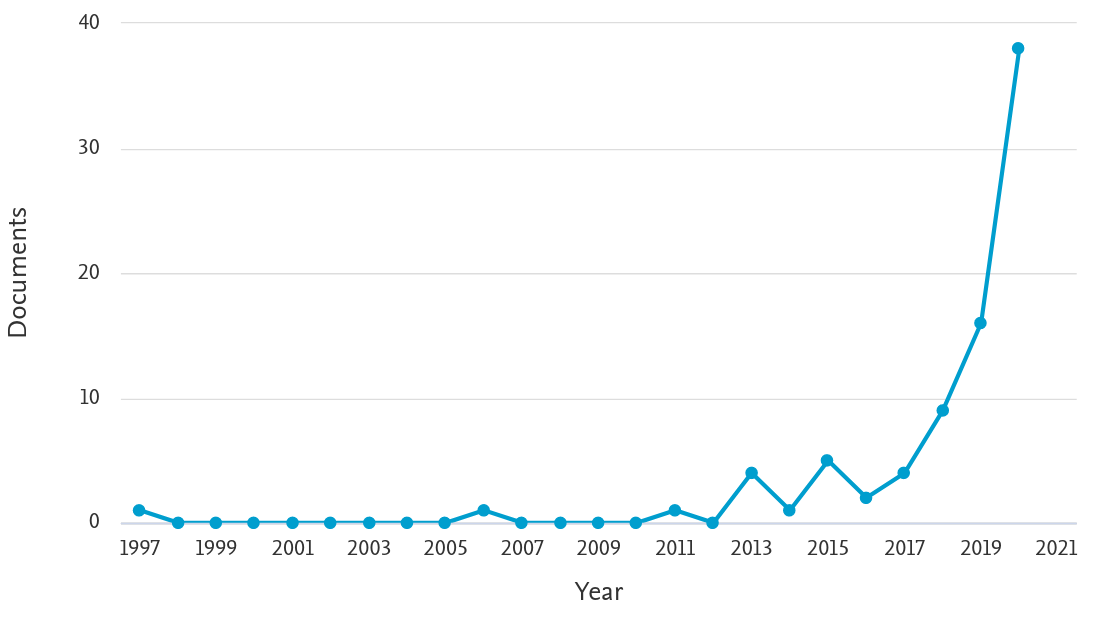
\includegraphics[width=\textwidth]{imagenes/scopus.png}
    \caption{Número de publicaciones relacionadas con aprendizaje por refuerzo y control HVAC en período 1997-2021}
    \label{fig:scopus}
\end{figure}

Este crecimiento se ha visto favorecido por los recientes avances en el campo del aprendizaje por refuerzo, y es que en los últimos años se ha demostrado la factibilidad del control HVAC mediante DRL empleando espacios de acciones reducidos y modelos de edificios simplificados \cite{zhang2019whole, vazquez2019fusing, moriyama2018reinforcement}.

La mayoría de las propuestas en la literatura destinadas a control HVAC mediante DRL hacen uso de diferentes herramientas de simulación energética de edificios, tales como EnergyPlus \cite{wetter2019ibpsa} o Modelica \cite{bucsoniu2018reinforcement}, facilitando así el entrenamiento y la experimentación. El uso de este tipo de simuladores se debe a que el entrenamiento de un agente de DRL en un escenario real sería demasiado ineficiente, debido a la necesidad de establecer un mapeo completo entre estados, acciones y recompensas considerando casos extremos \cite{brandi2020deep}. Además, se requiere de un entrenamiento de entre 20 y 50 días para converger en una política de control aceptable \cite{fazenda2014using, costanzo2016experimental, vazquez2019fusing}, lo que dificulta aún más el entrenamiento directo de algoritmos de DRL en entornos reales. Normalmente, los simuladores suelen combinarse con librerías de \textit{deep learning} (ej. TensorFlow/Keras, Pytorch) o DRL directamente (ej. Stable Baselines, RLlib) para pre-entrenar y probar los algoritmos en los entornos simulados antes de su despliegue \cite{wang2017long, valladares2019energy}.

\subsection{Formulación del problema}
\label{sec:formulacion}

Uno de los principales motivos que empujan al uso de DRL en control HVAC es la búsqueda de \textbf{ahorro energético}. De hecho, los sistemas basados en DRL han logrado conseguir una mayor eficiencia en comparación con los controladores tradicionales basados en reglas \cite{brandi2020deep, zhang2019whole, zhang2018deep, vazquez2019fusing, vazquez2017balancing}.

Por otro lado, los algoritmos de DRL destinados a control HVAC no tienen como único fin reducir el consumo energético, sino también garantizar una serie de requisitos de temperatura o \textbf{confort}\footnote{Es importante destacar que la definición de los estados o recompensas puede contemplar otras variables más allá de la temperatura tales como, por ejemplo, la concentración de CO$_2$ en el aire o la humedad.} \cite{wei2017deep, fazenda2014using, dalamagkidis2007reinforcement}.

Existen diferentes formas de medir el confort, tales como:

 \begin{itemize}
    \item La distancia entre la temperatura actual y la deseada: 
    
        \begin{equation}
            f(T, \hat{T}) = |T - \hat{T}|
        \end{equation}
        
    \item La distancia al cuadrado:
    
        \begin{equation}
            f(T, \hat{T}) = (T - \hat{T})^2
        \end{equation}
    
    \item La distancia a un rango de \textit{confort} objetivo:
    
        \begin{equation}
            f(T, T_{lower}, T_{upper}) = |T - T_{inf}|_+ + |T - T_{sup}|
        \end{equation}
    
    \item La distancia a la temperatura objetivo y al rango de confort según el estándar 55 de ASHRAE \cite{ansi2004standard}, el cual define un rango de temperatura aceptable de entre 23--26ºC para verano y 20--23.5ºC para invierno. Esto es:
    
        \begin{equation}
            f(T, \hat{T}, T_{inf}, T_{sup}) = |T - \hat{T}|_+ + (T - T_{sup})_+^2 + (T - T_{inf})^2
        \end{equation}
    
    \item Funciones no lineales como \textit{softplus}, gaussiana truncada, etc.
\end{itemize}

Mientras que algunos autores consideran que el confort de los ocupantes de un edificio es una restricción a la que siempre hay que dar prioridad, otros se centran en lograr un equilibrio entre dicho confort y el consumo de energético \cite{vazquez2019reinforcement}. 

Por tanto, el objetivo perseguido en el control HVAC de edificios no es otro que el de encontrar la política óptima que maximice el confort y minimice el consumo energético al mismo tiempo. Concretamente, buscamos una política, $\pi$, que implique la mayor cantidad de estados deseables posible y la menor cantidad de acciones energéticamente costosas.

Así, partiendo de un conjunto de \textbf{estados} u observaciones definidos por las condiciones ambientales del entorno, se plantean los siguientes objetivos:

\begin{itemize}
    
    \item Con respecto al consumo energético (medido en \textit{kWh}), buscamos la política que conduzca a su minimización, esto es:
        \begin{equation}
            \pi^* = \underset{\pi_\theta}{argmin}\sum^T_{t=1}\ coste(A_t)
        \end{equation}

    \item En el caso del confort, buscamos minimizar la diferencia entre el estado actual del edificio y el objetivo. Podemos definirlo tal que:
        \begin{equation}
            \pi^* = \underset{\pi_\theta}{argmin}\sum^T_{t=1}\ f(S_t, S_{objetivo})
        \end{equation}
    
    Un estado será deseable si las variables o condiciones ambientales que lo componen se encuentran dentro de las preferencias del usuario. Decimos que se produce una \textit{violación del confort} si la temperatura en el estado actual se encuentra fuera de los límites definidos por el usuario.
    
\end{itemize}

Vistos los objetivos a perseguir, podemos combinar la minimización del consumo energético y la maximización del confort en una sola expresión:

\begin{equation}
    \pi^* = \underset{\pi_\theta}{argmin}\sum^T_{t=1} w_t \cdot f(S_t,S_{objetivo}) + (1 - w_t) \cdot coste(A_t)
\end{equation}

siendo $w_t$ y $(1 - w_t)$ los pesos asignados a confort y consumo\footnote{Como puede observarse, $w$ puede ser variable en el tiempo ($w_t$) o incluso depender de otras variables como, por ejemplo, el número de ocupantes del edificio.}, respectivamente. Sobre esta base, podemos definir nuestra función de \textbf{recompensa} tal que:

\begin{equation}
    \label{eq:reward}
    r(S_t,A_t) = (1-w_t) \cdot \lambda_e \cdot coste(A_t) + w_t \cdot \lambda_c \cdot f(S_t,S_{objetivo})
\end{equation}

donde $coste(A_t)$ es el consumo energético; $f(S_t, S_{objetivo})$ es la función que mide el confort; $w$ y $(1-w)$ son los pesos asignados a cada parte de la recompensa, y $-\lambda_e$ (medido en $1/W$) y $-\lambda_c$ (medido en $1/\text{º}C$), sendos factores de escala empleados para eliminar las dimensiones del consumo y la temperatura\footnote{Es común definir dicha función de recompensa en términos negativos con el fin de que el objetivo sea maximizarla (aproximarla a $0$). Esto es: $r(S_t,A_t) = - (1-w_t) \cdot \lambda_e \cdot coste(A_t) - w_t \cdot \lambda_c \cdot f(S_t,S_{objetivo})$. Se trata de la función de recompensa estándar empleada internamente por Energym.}.

Finalmente, las \textbf{acciones} a realizar sobre el entorno y que darán lugar a una determinada recompensa dependerán del problema al que nos encontremos. En el problema tratado en este trabajo, las acciones consistirán en ajustar los \textit{setpoints} de calefacción y refrigeración, tal y como es habitual en control HVAC \cite{vazquez2017balancing, wei2017deep, fazenda2014using}. Un \textit{setpoint} marca la temperatura límite a partir de la cual deberá activarse un sistema de calefacción o refrigeración. En caso de fijar un \textit{setpoint} para calor y otro para frío, el objetivo será mantener el edificio dentro del intervalo entre ambos valores. Cabe destacar que, dependiendo del tipo de problema, el espacio de acciones podrá ser:

\begin{itemize}
    \item \textbf{Discreto}: existe un número finito de acciones donde cada acción es una tupla con valores de \textit{setpoints} fijos.
    \item \textbf{Continuo}: cada \textit{setpoint} es un número real a ajustar.
\end{itemize}

Finalmente, no todos los problemas de control HVAC residen en el ajuste de \textit{setpoints}: otras posibles acciones podrían consistir en regular la potencia de ventilación, o la apertura y cierre de ventanas \cite{chen2018optimal}, entre muchas otras. 

En conclusión, todo problema de control HVAC destinado a ser resuelto mediante RL cuenta con los siguientes componentes:

\begin{itemize}
    \item Una serie de \textbf{estados} u observaciones compuestos por las condiciones ambientales del entorno: temperatura externa/interna, humedad, luminosidad, concentración de CO$_2$, etc., en un momento dado.
    \item Una función de \textbf{recompensa} donde se combinan de forma ponderada el consumo energético (a minimizar) y el confort (a maximizar).
    \item Un espacio de \textbf{acciones} consistentes, en este caso, en la regulación de los \textit{setpoints} para calefacción y refrigeración. Dicho espacio de acciones puede ser discreto o continuo.
\end{itemize}

\subsection{Estado del arte}
\label{sec:estado-del-arte}

Una vez introducido el uso de DRL en control HVAC, pasamos a revisar algunas de las aportaciones más novedosas de la literatura científica en los últimos años.

En el año 1997 tenemos la primera aproximación al uso de RL en control HVAC de la mano de Anderson et al. \cite{anderson1997synthesis}. En este trabajo, se propuso el uso de RL en combinación con control proporcional-integral (PI) para el control de una bobina de calor (\textit{heating coil}). Un año más tarde, en 1998, tuvo lugar la primera aplicación directa de RL en control HVAC, \cite{mozer1998neural}, donde Mozer expuso su \textit{Neural Network House} basada en el control automático de agua caliente, HVAC e iluminación, buscando así reducir el consumo energético y garantizar el bienestar de sus ocupantes.

Desde ese momento, se han ido desarrollando una gran cantidad de trabajos centrados en la reducción del gasto energético de edificios y su gestión inteligente. Algunos ejemplos son: \cite{sun2015event}, donde se consiguió minimizar el consumo energético en un entorno con múltiples estancias; \cite{liu2006experimental,liu2007evaluation}, donde se proponen métodos híbridos orientados a gestionar sistemas de agua fría en grandes centros comerciales, o \cite{costanzo2016experimental}, centrado en la reducción del consumo energético en sistemas de aire acondicionado.

Un factor importante a considerar en la regulación de \textit{setpoints} para calefacción y refrigeración es la ocupación de los edificios. Este factor fue considerado por Barrett \& Linder en \cite{barrett2015autonomous}, donde consiguieron reducir en un 10\% los costes energéticos derivados de dispositivos HVAC empleando RL. De forma similar, en el caso de \cite{urieli2013learning, ruelens2015learning}, se investigaron métodos basados en \textit{set-back} orientados a relajar los requisitos de temperatura cuando no hay personas en el edificio.

Otros ejemplos de aplicaciones de RL destinadas a incrementar la conservación de energía en edificios son \cite{li2015multi, vazquez2017balancing, vazquez2019fusing, dalamagkidis2007reinforcement, yu2010online, yuan2020study, azuatalam2020reinforcement} donde tanto el ahorro energético como el confort fueron tenidos en cuenta para optimizar el funcionamiento de dispositivos HVAC en diferentes entornos. En \cite{brandi2020deep}, se logró un ahorro de entre un 5\% y un 12\% en el control del sistema de calefacción de un edificio de oficinas haciendo uso de un agente basado en \textit{Double DQN}. Por otro lado, Zhang et al. \cite{zhang2019whole, zhang2018deep} lograron reducir en un 16.7\% la demanda energética en un edificio de oficinas empleando A3C, mientras que Vázquez-Canteli et al. \cite{vazquez2019fusing, vazquez2017balancing} lograron un 10\% de ahorro energético aplicando DQN en el control de una bomba de calor. Destaca el caso de Dalamagkidis et al. \cite{dalamagkidis2007reinforcement}, donde los niveles de CO$_2$ también se tuvieron en cuenta como métrica de confort.

Un trabajo reciente y de especial interés es el de Azuatalam et al. \cite{azuatalam2020reinforcement}, donde se llevó a cabo una completa revisión del estado del arte en control HVAC mediante RL, proponiendo una arquitectura capaz de alcanzar un 22\% de ahorro energético semanal.

Finalmente, en \cite{du2008two}, se propone un modelo \textit{actor-critic} orientado a reducir el error en el ajuste de \textit{setpoints} de sistemas HVAC, mientras que en \cite{henze2003evaluation} se llevó a cabo una investigación orientada a probar la eficacia del RL en sistemas de almacenamiento de frío en edificios comerciales.

Como puede verse, contamos con una importante base teórica y práctica sobre la cual se fundamenta el control HVAC por medio de RL y DRL. En esta sección se ha tratado de reflejar parte de la literatura existente, mostrando el amplio abanico de posibilidades que este campo ofrece, y abriendo la puerta al lector a consultar recientes revisiones de la literatura como \cite{vazquez2019reinforcement, mason2019review} en caso de buscar una mayor profundización.

Ya mencionamos en el Capítulo \ref{ch:1} que la mayor parte de los sistemas de control HVAC basados en RL y DRL presentes en la literatura son difícilmente reproducibles y comparables \cite{vazquez2019reinforcement}. No existe, hasta el momento, ningún \textit{framework} (más allá de los brevemente propuestos en \cite{vazquez2019reinforcement}, \cite{azuatalam2020reinforcement}) o \textit{benchmark} destinados a constituir un marco común desde el que comparar modelos de RL y DRL en diferentes climas y entornos. Así, tomando como referencia la arquitectura basada en OpenAI Gym y EnergyPlus propuesta por Zhang et al. en \cite{zhang2018practical, zhang2019whole}, el objetivo de este trabajo será proponer una solución a este problema, tratando de desarrollar un ecosistema de simulación común que pueda ser empleado para validar cualquier nueva aportación al campo.




\chapter{Desarrollo de Energym}
\label{ch:3}

En este capítulo abordaremos el proceso de desarrollo de Energym, así como las principales aportaciones realizadas en su implementación y mejora.

\section{Introducción a Energym}

Tal y como se ha adelantado en los anteriores capítulos, el principal objetivo de este proyecto consistió en el desarrollo de un entorno de ejecución de simulaciones energéticas adaptado para su uso con algoritmos de aprendizaje por refuerzo. 

Nace así \textbf{Energym}, basado en la interfaz de OpenAI Gym\footnote{OpenAI Gym es una interfaz de programación destinada al desarrollo de entornos empleados en aprendizaje por refuerzo: \url{https://gym.openai.com/}.} y destinado a servir como un marco de pruebas estándar sobre el que ejecutar algoritmos de RL/DRL en diferentes edificios y climas, favoreciendo así su evaluación y comparación. El proyecto tiene su origen en el entorno \href{https://github.com/zhangzhizza/Gym-Eplus}{Gym-Eplus} de Zhang \& Lam \cite{zhang2019whole, zhang2018practical}, cuyo \textit{back-end} fue tomado como referencia para ofrecer una nueva versión actualizada, escalable y fácilmente reutilizable.

Veamos las principales aportaciones de Energym:

\begin{itemize}
    \item \textbf{Entornos de \textit{benchmarking}}. Al igual que los entornos \href{https://gym.openai.com/envs/\#atari}{Atari} o \href{https://gym.openai.com/envs/\#mujoco}{MuJoCo} ampliamente utilizados por la comunidad de RL, Energym incorpora un conjunto de entornos para la evaluación, comparativa y prueba de algoritmos de RL/DRL en control energético de edificios. Estos entornos incluyen diferentes edificios, climas y espacios de acciones.
    \item \textbf{Flexibilidad en la experimentación}. Energym permite la personalización de diferentes aspectos de la simulación, tales como la función de recompensa empleada o la selección de las variables que conforman las observaciones de los agentes.
    \item \textbf{Compatibilidad con diferentes motores de simulación}. Aunque actualmente sólo se ha implementado la conexión con \href{https://energyplus.net/}{EnergyPlus}, el objetivo es que Energym pueda ser empleado con diferentes motores de simulación, como \href{https://www.openmodelica.org/}{OpenModelica} o \href{https://es.mathworks.com/products/simulink.html}{Simulink}.
    \item \textbf{Integración con \href{https://stable-baselines3.readthedocs.io}{Stable Baselines3}}. Energym cuenta con diferentes funcionalidades adaptadas a esta librería de RL (ej. \textit{callbacks}) con el fin de poder probar fácilmente los entornos implementados.
\end{itemize}

Una vez definidas las principales características de Energym, pasemos a estudiar su funcionamiento. Como se muestra en la Figura \ref{fig:energym-ecosystem}, el ecosistema de simulación planteado consta de los siguientes elementos:

\begin{figure}
    \centering
    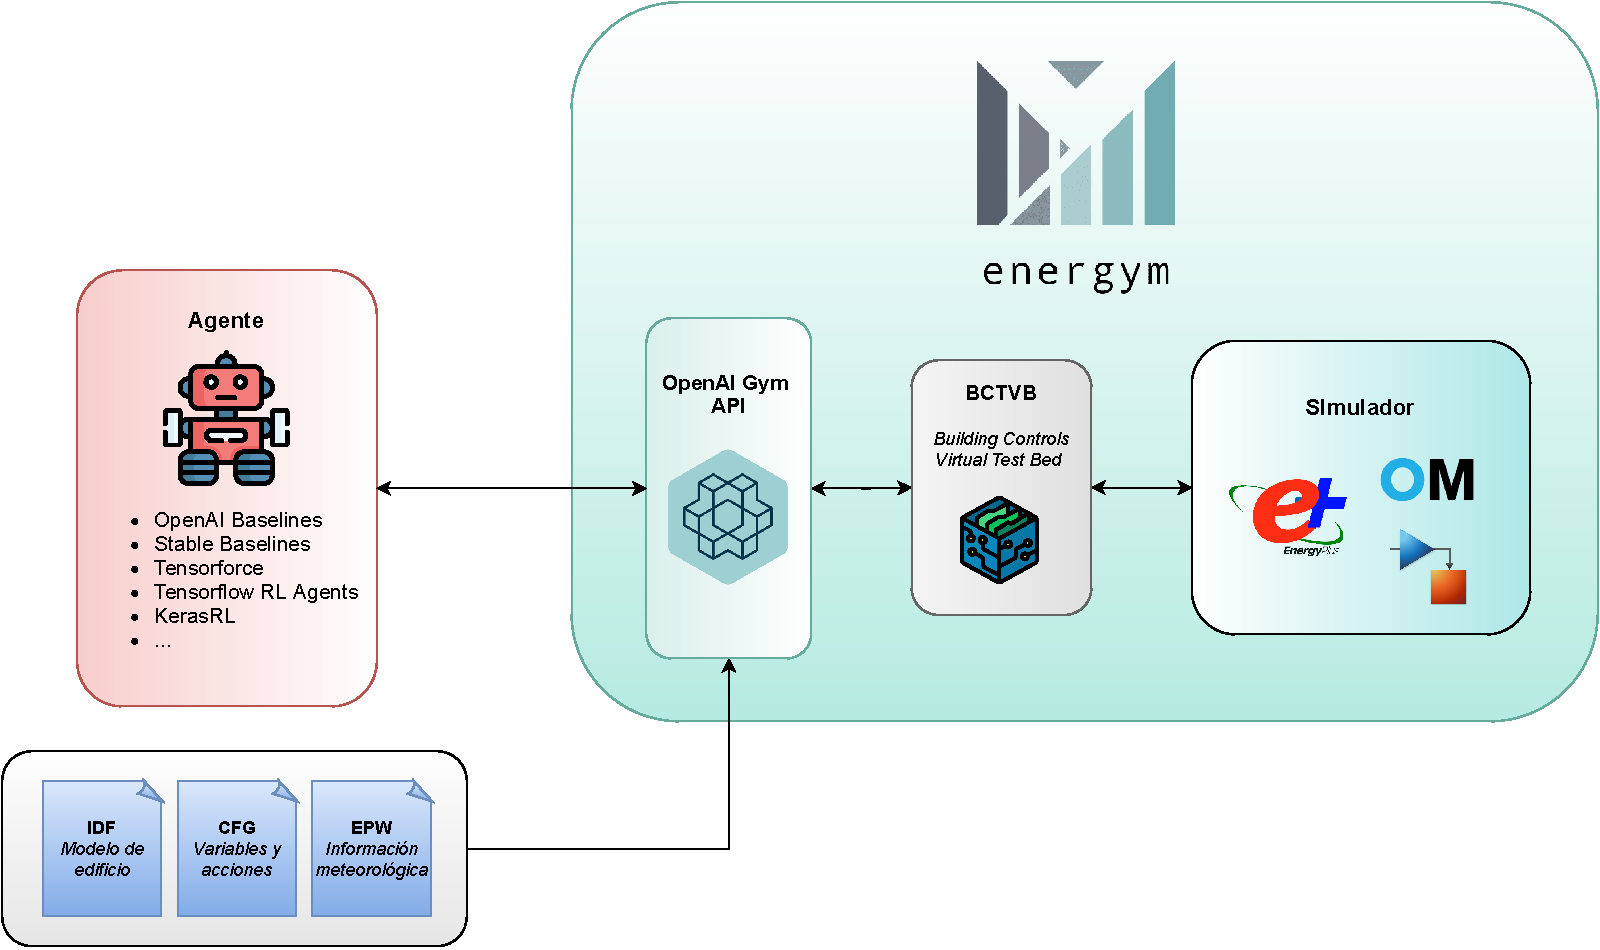
\includegraphics[width=\textwidth]{imagenes/energym-diagram.pdf}
    \caption{Elementos que componen el ecosistema de Energym}
    \label{fig:energym-ecosystem}
\end{figure}

\begin{itemize}
    \item Un \textbf{agente} que interactúa con el entorno. Su implementación puede llevarse a cabo mediante diferentes librerías de DRL, tales como \href{https://github.com/openai/baselines}{OpenAI Baselines}, \href{https://github.com/DLR-RM/stable-baselines3}{Stable Baselines}, \href{https://www.tensorflow.org/agents}{Tensorflow Agents},  \href{https://github.com/keras-rl/keras-rl}{KerasRL}, etc.
    \item Una serie de \textbf{ficheros de configuración} que serán empleados en la simulación:
        \begin{itemize}
            \item Un fichero \texttt{.idf} (\textit{Input Data File}, IDF) con el modelo del edificio empleado en la simulación.
            \item Un fichero \texttt{.cfg} con información sobre las acciones, variables de entrada y salida a emplear, sus rangos, etc.
            \item Un fichero \texttt{.epw} (\href{https://energyplus.net/weather}{\textit{EnergyPlus Weather}}, EPW) con información meteorológica empleada en la simulación.
        \end{itemize}
    Todo entorno queda definido por el edificio, variables de entrada y salida, tipos de acciones (discretas o continuas) y clima especificados en estos ficheros.
    \item El entorno de simulación \textbf{Energym}, desarrollado bajo la interfaz de OpenAI Gym y conectado a un simulador (EnergyPlus, OpenModelica, Simulink...) por medio de BCTVB (\textit{Building Controls Virtual Test Bed}). BCVTB es un \textit{middleware} \textit{open source} que permite el acoplamiento de diferentes sistemas de simulación distribuidos. En nuestro caso, su uso reside en la conexión entre el entorno de simulación y el simulador empleado\footnote{Para más información, consúltese: \url{https://simulationresearch.lbl.gov/bcvtb}.}.
\end{itemize}

Así, la interacción entre estos elementos se realiza tal y como se muestra en la Figura \ref{fig:operation-diag}: el agente interactúa con Energym modificando una serie de variables de entrada y recibe observaciones con el valor de las variables de salida proporcionadas tras la simulación. Por otro lado, en base a las dinámicas del entorno se genera una recompensa que el agente tratará de maximizar.

\begin{figure}
    \centering
    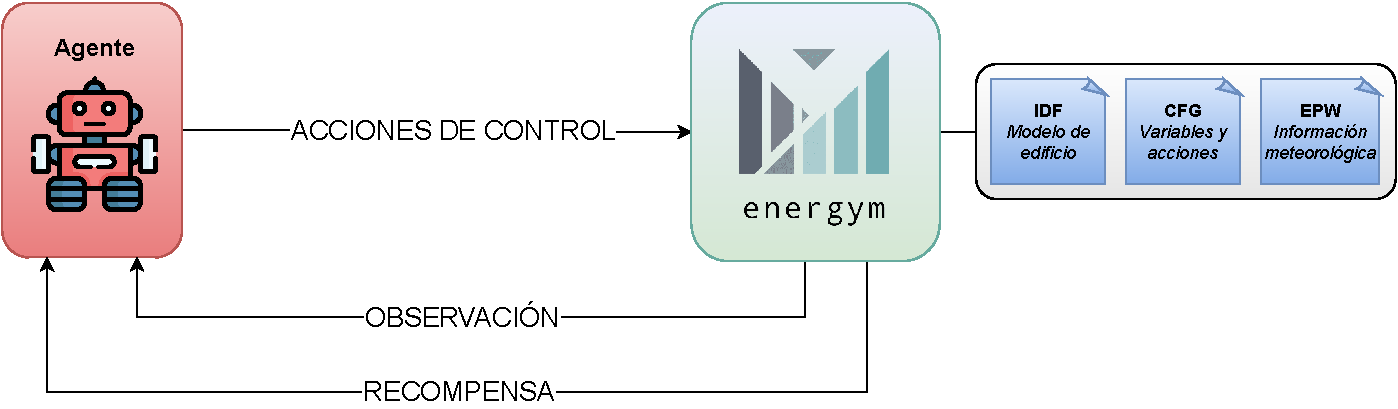
\includegraphics[width=\textwidth]{imagenes/operation-diagram.pdf}
    \caption{Proceso de simulación}
    \label{fig:operation-diag}
\end{figure}

Cabe destacar que, hasta el momento, no existe ninguna propuesta similar a Energym, lo que supone una importante contribución en este campo. Además, el hecho de distribuirse como código abierto abre la oportunidad a futuras aportaciones por parte de usuarios interesados en colaborar en su desarrollo. El principal objetivo de Energym es ofrecer un entorno de simulación sencillo, eficiente y flexible, de tal forma que cualquier usuario que desee utilizarlo en sus propios proyectos pueda descargar el código y modificar la configuración para adecuar Energym a sus objetivos.

Finalmente, Energym abre la puerta a un gran número de posibles experimentaciones: comparativa de algoritmos de RL/DRL sobre unas mismas condiciones; estudio de la influencia del clima en el control energético; análisis de las variables que más influyen en el aprendizaje; comparativa de desempeño para espacios de acciones discretos y continuos, y un largo etcétera.

\section{Organización y metodología de trabajo}

La implementación de Energym llevada a cabo en el marco de este proyecto supuso la colaboración como parte de su equipo de desarrollo. Así, partiendo de un proyecto iniciado el 23 de enero de 2021 y una serie de ideas generales sobre los objetivos a perseguir, se pasó a formar parte de su desarrollo.

El equipo de trabajo del cual se pasó a formar parte durante esta parte del trabajo estuvo compuesto por los siguientes integrantes:

\begin{itemize}
    \item Javier Jiménez: creador del proyecto, encargado de gestionar el repositorio de Energym, así como de dirigir su desarrollo en líneas generales.
    \item Alejandro Campoy: incorporado al desarrollo de Energym a partir del 12 de abril.
    \item Juan Gómez y Miguel Molina: supervisores del proyecto.
\end{itemize}

La colaboración con el equipo de desarrollo se llevó siguiendo una comunicación continua por medio de herramientas colaborativas como Slack o GitHub. No se trató de un desarrollo al uso, sino que se siguió una forma de trabajo propia de entornos profesionales, siguiendo una metodología de desarrollo basada en \textit{issues}/\textit{pull requests}, integración continua, versionado y desarrollo en ramas independientes, etc. En las Figuras \ref{fig:git1}, \ref{fig:git2} y  \ref{fig:git3} se muestra una perspectiva general del repositorio.

\begin{figure}
    \centering
    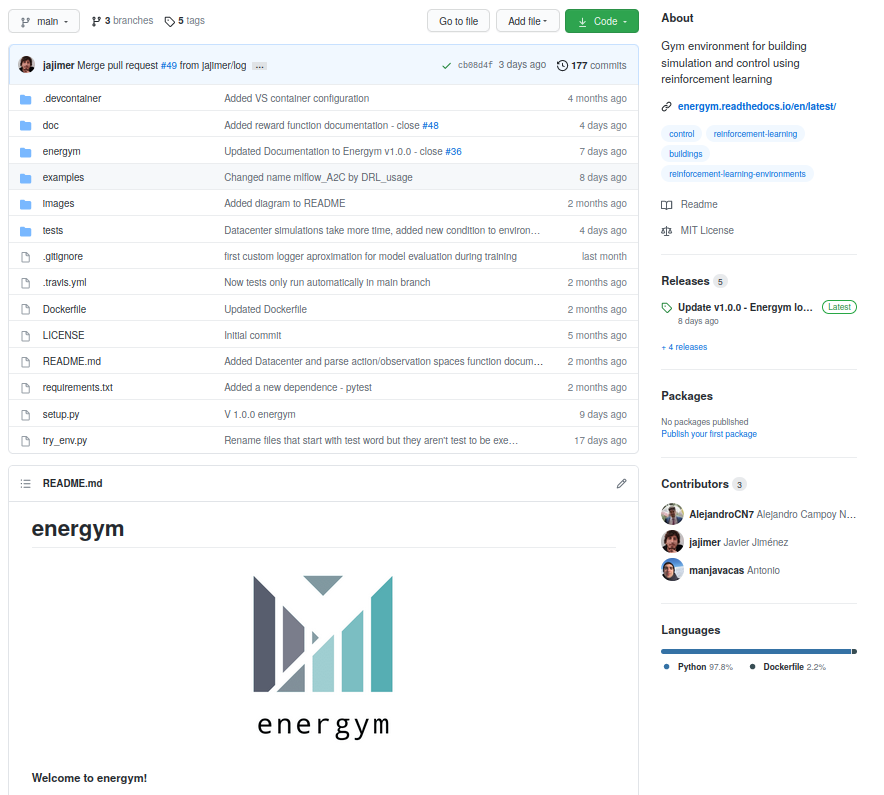
\includegraphics[width=\textwidth]{imagenes/git.png}
    \caption{Repositorio de Energym en GitHub}
    \label{fig:git1}
\end{figure}

\begin{figure}
    \centering
    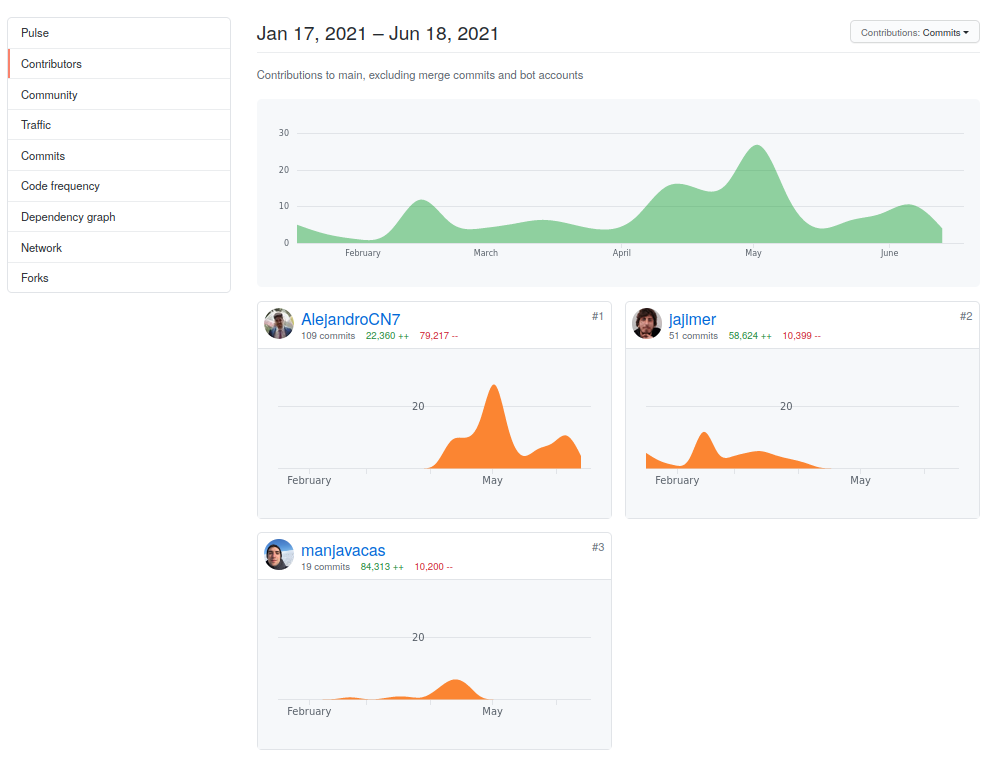
\includegraphics[width=\textwidth]{imagenes/git-contributions.png}
    \caption{Contribuciones al repositorio}
    \label{fig:git2}
\end{figure}

\begin{figure}
    \centering
    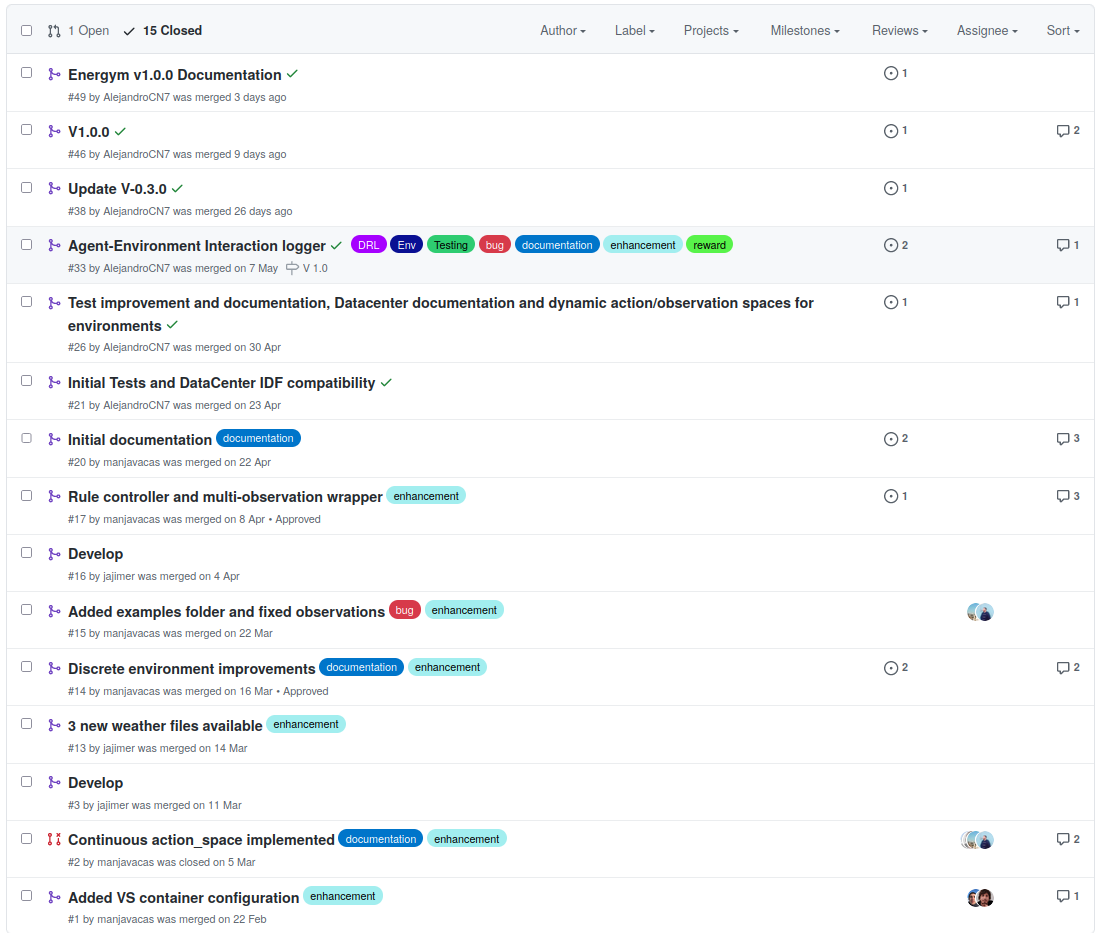
\includegraphics[width=\textwidth]{imagenes/git-pull-requests.png}
    \caption{Desarrollo basado en \textit{pull requests}}
    \label{fig:git3}
\end{figure}

En la Figura \ref{fig:git2} puede observarse cómo la primera parte del desarrollo fue principalmente llevada a cabo por Javier Jiménez, creador del proyecto; posteriormente, el autor de este trabajo tomó el relevo en su implementación (puede verse una mayor frecuencia de contribuciones entre febrero y mayo) para, posteriormente, dar el relevo a Alejandro Campoy como principal desarrollador desde el mes de abril.

\section{Contribuciones al desarrollo}

Como parte de las aportaciones realizadas en el desarrollo de Energym, destacan las siguientes tareas:

\subsection{Imagen Docker}

Un primer paso fue la implementación de la imagen Docker empleada para desarrollar y utilizar Energym, facilitando la gestión de dependencias y el desarrollo dentro de un entorno aislado. 
    
Docker permite el despliegue de aplicaciones en contenedores, ofreciendo modularidad, una rápida implementación y un desarrollo flexible. Simplemente es necesario definir un fichero Dockerfile donde se especifiquen las operaciones a realizar una vez inicializado el contenedor (instalación de dependencias, declaración de variables de entorno, etc.) para, posteriormente, poder interactuar con el entorno virtualizado que Docker ofrece.
    
Así, se propuso la implementación de una imagen Docker que permitiese utilizar Energym en un entorno cerrado, gestionándose de forma automática aspectos tales como la instalación de EnergyPlus y BCVTB, o la declaración de las variables de entorno empleadas por Energym. 
    
Finalmente, se incluyó en el repositorio la configuración necesaria para automatizar la construcción y despliegue del contenedor en Visual Studio Code de forma rápida y sencilla.

\subsection{Desarrollo de entornos de simulación}
\label{sec:entornos}
    
Posteriormente, se procedió al desarrollo de los entornos basados en espacios de acciones continuos y discretos. Como ya mencionamos en la sección \ref{sec:formulacion}, el problema de regulación de \textit{setpoints} en control HVAC puede formularse considerando un espacio de acciones discreto o continuo. El objetivo perseguido en el desarrollo de Energym fue el de implementar ambos, de cara a evaluar el desempeño de algoritmos de DRL que únicamente operan en un tipo de espacio de acciones (por ejemplo, DQN en entornos discretos, o DDPG en continuos). Otro objetivo considerado fue el de evaluar los resultados obtenidos por un mismo algoritmo en cada tipo de entorno (por ejemplo, A2C).
    
Para los entornos basados en acciones discretas, los rangos de temperatura se fijaron de acuerdo a los propuestos en \cite{center2013determining}. En este caso, un total de 10 configuraciones componen el espacio de acciones\footnote{Los espacios de acciones pueden configurarse a voluntad modificando el fichero \texttt{.cfg} empleado por Energym.}, donde cada una está compuesta por una tupla $<setpoint_{calor},\ setpoint_{frio}>$ (ver Tabla \ref{tb:disc-actions}).
    
    \begin{table}
        \centering
        \caption{Espacio de acciones discreto empleado por defecto}
        \label{tb:disc-actions}
        \begin{tabular}{ccc}
        N & \textit{Setpoint calor} & \textit{Setpoint frío} \\ \hline
        0 & 15 & 30 \\ \hline
        1 & 16 & 29 \\ \hline
        2 & 17 & 28 \\ \hline
        3 & 18 & 27 \\ \hline
        4 & 19 & 26 \\ \hline
        5 & 20 & 25 \\ \hline
        6 & 21 & 24 \\ \hline
        7 & 22 & 23 \\ \hline
        8 & 22 & 22 \\ \hline
        9 & 21 & 21 \\ \hline
        \end{tabular}
    \end{table}
    
Con respecto a los entornos continuos, el ajuste de los \textit{setpoints} quedó acotado a los intervalos que se muestran en la Tabla \ref{tb:cont-actions}. Dentro de dichos intervalos, cada \textit{setpoint} podrá tomar un valor continuo determinando, lo que incrementa más que considerablemente el número de combinaciones acción--estado que podrán darse dentro del entorno.
    
\begin{table}
    \centering
    \caption{Espacio de acciones continuo empleado por defecto}
    \label{tb:cont-actions}
    \begin{tabular}{llll}
    N & \textit{Setpoint} & Mín. & Max. \\ \hline
    0 & Calor & 15,0 & 22,5 \\ \hline
    1 & Frío & 22,5 & 30,0 \\ \hline
    \end{tabular}
\end{table}

Una vez visto el tipo de acciones que podemos ejecutar sobre el entorno, otros elementos configurables empleados por Energym son: las \textbf{variables} que definen una observación, el \textbf{edificio} empleado para la simulación, y el \textbf{clima}, los cuales abordaremos en detalle en el Capítulo \ref{ch:4}. Además, es posible (y recomendable de cara a favorecer la generalización en el aprendizaje) simular entornos estocásticos donde los datos meteorológicos presentes en el fichero \texttt{.epw} son ligeramente modificados en cada episodio a partir de \textbf{ruido} gaussiano (con media $0$ y desviación estándar $2,5$).

Finalmente, los entornos de simulación considerados en este proyecto son los mostrados en la Tabla \ref{tb:entornos}, de acuerdo a las posibles combinaciones de espacio de acciones y clima\footnote{Tipos de clima acordes a la clasificación del \href{https://www.energycodes.gov/development/commercial/prototype_models}{DOE}.}. Profundizaremos en estos ellos en el Capítulo \ref{ch:4}.
   
%%%

\begin{landscape}
    \begin{table}
    \centering
    \caption{Entornos empleados en este proyecto}
    \label{tb:entornos}
    \begin{tabular}{llllll}
    \multicolumn{1}{c}{\textbf{Entorno}} & \multicolumn{1}{c}{\textbf{Localización}} & \multicolumn{1}{c}{\textbf{IDF}} & \multicolumn{1}{c}{\textbf{Clima}} & \multicolumn{1}{c}{\textbf{Acciones}} & \multicolumn{1}{c}{\textbf{Período}} \\ \hline
    Eplus-discrete-stochastic-hot-v1 & Arizona, USA & 5ZoneAutoDXVAV.idf & Hot dry (2B) + ruido & Discrete(10) & 01/01 - 31/12 \\
    Eplus-discrete-stochastic-mixed-v1 & New York, USA & 5ZoneAutoDXVAV.idf & Mixed humid (4A) + ruido & Discrete(10) & 01/01 - 31/12 \\
    Eplus-discrete-stochastic-cool-v1 & Washington, USA & 5ZoneAutoDXVAV.idf & Cool marine (5C) + ruido & Discrete(10) & 01/01 - 31/12 \\ \hline
    Eplus-continuous-stochastic-hot-v1 & Arizona, USA & 5ZoneAutoDXVAV.idf & Hot dry (2B) + ruido & Box(2) & 01/01 - 31/12 \\
    Eplus-continuous-stochastic-mixed-v1 & New York, USA & 5ZoneAutoDXVAV.idf & Mixed humid (4A) + ruido & Box(2) & 01/01 - 31/12 \\
    Eplus-continuous-stochastic-cool-v1 & Washington, USA & 5ZoneAutoDXVAV.idf & Cool marine (5C) + ruido & Box(2) & 01/01 - 31/12 \\ \hline
    \end{tabular}%
    \end{table}
\end{landscape}

%%%

\subsection{Gestión de los ficheros de configuración}

Esta tarea supuso la lectura y adaptación de los ficheros de configuración (\texttt{.idf}, \texttt{.cfg} y \texttt{.epw}) utilizados por Energym. Por un lado, requirió la búsqueda y uso de librerías destinadas a una lectura eficiente de los ficheros IDF empleados por Energym (por ejemplo, \href{https://pypi.org/project/opyplus/}{\textit{opyplus}}). También se realizaron modificaciones en el modelo de edificio para adaptarlo a la experimentación que posteriormente sería llevada a cabo, como la ampliación del período de simulación a 1 año.

Por otro lado, a las variables devueltas por EnergyPlus como observación en cada \textit{timestep} se añadieron valores adicionales, como la hora o fecha de cada día simulado. Esta información no sólo se incorporó como una variable más a emplear en el aprendizaje, sino también con el fin de añadir a las simulaciones una mayor trazabilidad y facilitar su estudio desde diferentes perspectivas temporales. Por ejemplo: considerar en qué meses el rendimiento obtenido es peor, si existe algún tipo de estacionalidad en la recompensa obtenida, etc.
    
\subsection{Limpieza y adaptación del \textit{back-end}}

De especial relevancia fue la limpieza y adaptación del código \textit{back-end} heredado del repositorio de \href{https://github.com/zhangzhizza/Gym-Eplus}{Gym-Eplus}. El \textit{back-end} de este proyecto fue reutilizado para establecer la conexión entre Energym y EnergyPlus a través de BCVTB, tal y como se muestra en la Figura \ref{fig:backend}.
    
\begin{figure}
    \centering
    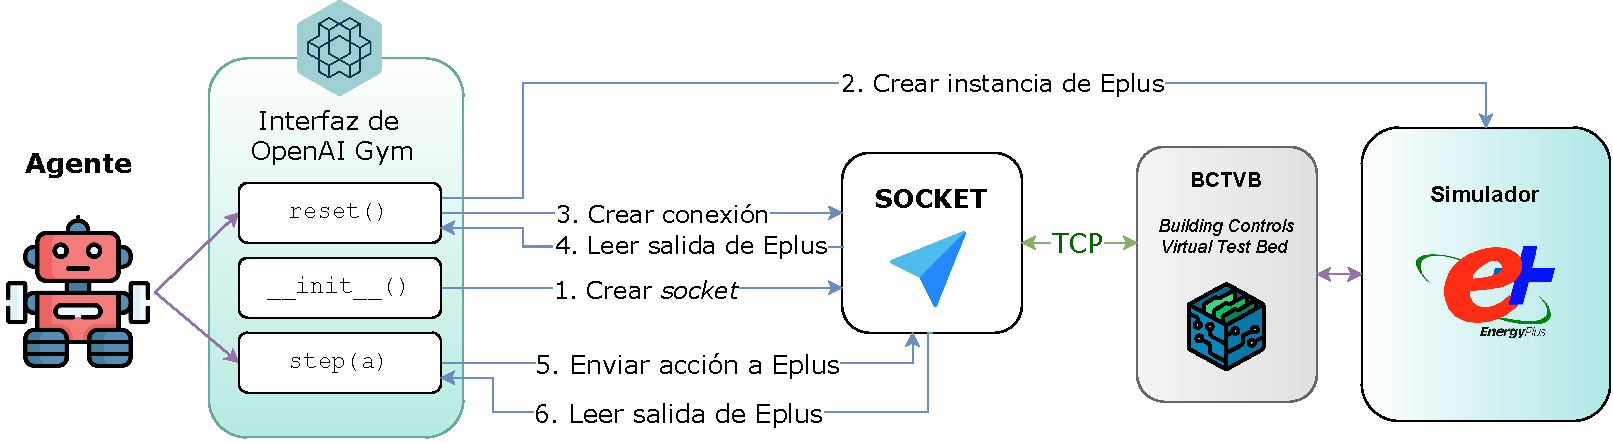
\includegraphics[width=\textwidth]{imagenes/backend.pdf}
    \caption{Interacción con el \textit{back-end} de Energym, heredado de Gym-Eplus. Imagen modificada de \cite{zhang2019whole}}
    \label{fig:backend}
\end{figure}

Al partir de código heredado, fue necesaria una completa interpretación del \textit{back-end} del proyecto original antes de abordar su adaptación y optimización. Posteriormente, se llevó a cabo su reorganización, eliminando aquellas partes de código no empleadas en nuestro proyecto y modificando otras para poder ser utilizadas con Energym. Finalmente, esta parte del proyecto pasó a ser documentada.

\subsection{Documentación}

De cara a contar con un documento de referencia que permitiese detallar el funcionamiento de Energym a la comunidad, se desarrolló la primera versión de la documentación de la librería utilizando \href{https://www.sphinx-doc.org}{\textit{Sphinx}}. Así, una vez implementado el núcleo funcional de Energym, se procedió a documentar sus principales componentes. \textit{Sphinx} ofrece numerosas facilidades para elaborar la documentación de código, siempre y cuando se parta de un código comentado en un formato estándar como \href{https://www.sphinx-doc.org/en/master/usage/extensions/example_numpy.html?highlight=numpy#example-numpy-style-python-docstrings}{Numpy} o \href{https://www.sphinx-doc.org/en/master/usage/extensions/example_google.html#example-google}{Google}.

La documentación generada fue publicada en la plataforma \href{readthedocs.org}{\textit{Read the Docs}} (ver Figura \ref{fig:readthedocs}), la cual permite su alojamiento de forma gratuita y la sincronización automática con el repositorio en el que se aloja el proyecto\footnote{La documentación de Energym se encuentra actualizada y puede consultarse en el siguiente enlace: \url{https://energym.readthedocs.io/}.}.

\begin{figure}
    \centering
    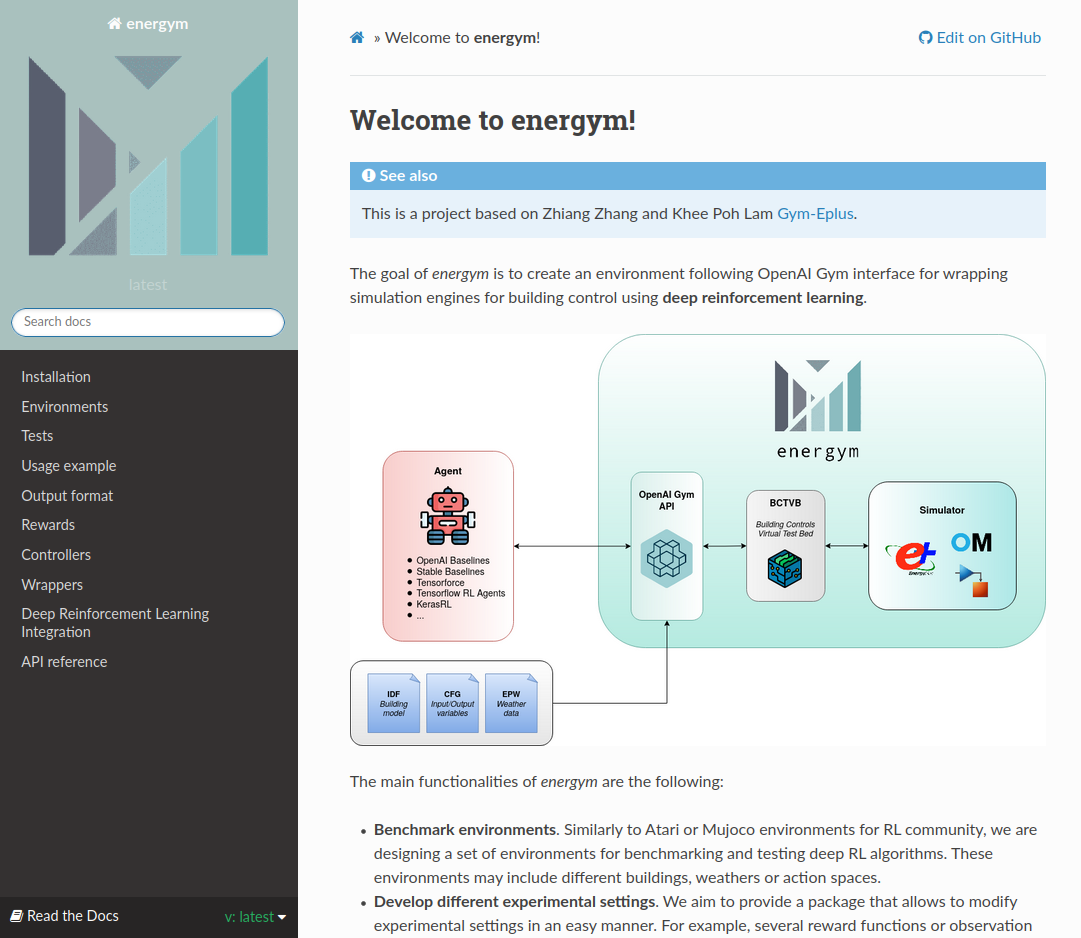
\includegraphics[width=\textwidth]{imagenes/readthedocs.png}
    \caption{Documentación de Energym alojada en \textit{Read the Docs}}
    \label{fig:readthedocs}
\end{figure}

Finalmente, a la elaboración de la documentación inicial se sumó la implementación de una serie \textit{scripts} de ejemplo destinados a ilustrar el funcionamiento de Energym en diferentes contextos. Estos serían empleados para probar la integración de Energym con MLflow y Tensorboard, ejemplificar el uso de \textit{wrappers}, o mostrar la integración de Energym con Stable Baselines3, como veremos más adelante.

\subsection{Controlador basado en reglas}
Un aspecto importante a la hora de poder evaluar la eficiencia de algoritmos de DRL en control HVAC es tener como referencia un controlador basado en reglas con respecto al cual poder comparar. Esta tarea supuso el desarrollo de dicho controlador, cuyo funcionamiento se detalla en el Algoritmo \ref{alg:reglas}. De nuevo, se tomaron como referencia los rangos de temperatura expuestos en \cite{center2013determining}.

\begin{algorithm}
\caption{Controlador basado en reglas}
\label{alg:reglas}
\DontPrintSemicolon
\LinesNumbered
\KwIn{$s$: una observación del entorno}
\KwOut{$accion$: la combinación de \textit{setpoints} a ajustar}

$t \leftarrow$ obtener temperatura exterior de $s$\;

    \If{$t < 15$}{
        $accion = (19,21)$\;
    }
    \ElseIf{$t < 20$}{
        $accion = (20,22)$\;
    }
    \ElseIf{$t < 26$}{
        $accion = (21,23)$\;
    }
    \ElseIf{$t < 30$}{
        $accion = (26,30)$\;
    }
    \Else{
        $accion = (24,26)$\;
    }

\Return{accion}

\end{algorithm}

Como puede observarse, un controlador basado en reglas ajusta los \textit{setpoints} en base a la temperatura exterior del entorno. La ventaja de este enfoque basado en reglas es su aplicabilidad en la mayoría de sistemas, la clara interpretación de las reglas, así como su flexibilidad para ajustarse a cualquier tipo de dispositivo HVAC \cite{mavrik2011advanced}. 

No obstante, este tipo de controladores suelen ser ineficientes en la práctica, debido a la complejidad de la dinámica térmica de los edificios y a las perturbaciones heterogéneas que puedan darse en el entorno. Tal y como se explica en \cite{wei2017deep, yang2015reinforcement}, el rendimiento y fiabilidad de estos enfoques dependen en gran medida de la precisión del modelo térmico del edificio, el cual no sólo debe ser preciso sino también eficiente. Además, la temperatura del edificio puede verse afectada por muchos factores no contemplados por estos sistemas, como la estructura y materiales del edificio, la humedad, la intensidad de la radiación solar o las ganancias de calor debidas a los ocupantes del edificio. Como resultado, la temperatura del edificio termina por presentar comportamientos aleatorios debido a una modelización incompleta. 

Concluimos, por tanto, enfatizando la dificultad para desarrollar un controlador basado en reglas lo suficientemente preciso y eficiente para un control eficaz de la climatización en tiempo real. De aquí parte la idea de desarrollar algoritmos de RL/DRL que traten de mejorar estas propuestas, siempre y cuando se parta de un control basado en reglas a partir del cual poder comparar los resultados obtenidos (tanto en términos de confort como de consumo).

\subsection{\textit{Wrappers}}

OpenAI Gym permite extender los entornos convencionales de forma modular por medio de \textit{wrappers}. Las clases que heredan de \texttt{gym.Wrapper} permiten al programador personalizar observaciones (\texttt{gym.ObservationWrapper)}, acciones (\texttt{gym.ActionWrapper)} y recompensas (\texttt{gym.RewardWrapper)}, sobrescribiendo sus implementaciones por defecto.

En el caso de Energym, se implementaron una serie de \textit{wrappers} de cara a extender las funcionalidades del entorno por defecto\footnote{Su implementación puede consultarse en: \url{https://github.com/jajimer/energym/blob/main/energym/utils/wrappers.py}}:

\begin{itemize}
    \item \texttt{NormalizeObservation}: \textit{wrapper} destinado a normalizar los valores de las variables que componen cada observación. El objetivo perseguido con este \textit{wrapper} es favorecer el entrenamiento de los algoritmos de DRL, reduciendo la variabilidad de los valores empleados. 
    
    Un problema inicial fue decidir qué rangos emplear para normalizar cada valor mediante min--max:
    
    \begin{equation}
        x_{norm} = \frac{x - min}{max - min}
    \end{equation}
    
    Para resolver este problema, se llevó a cabo una aproximación empírica basada la ejecución de múltiples simulaciones con un agente aleatorio. Partiendo de los registros de estas simulaciones, fue posible conocer los valores mínimo y máximo del dominio de cada variable, y emplearlos así para normalizar.
    
    Finalmente, se comprobó que este \textit{wrapper} mejoraba los resultados obtenidos por los agentes con respecto al uso de observaciones por defecto.
    
    \item \texttt{MultiObsWrapper}: este \textit{wrapper} permite agrupar múltiples observaciones y utilizar su información de forma combinada para favorecer el entrenamiento. Si bien se trata de un tipo de \textit{wrapper} especialmente útil en entornos como Atari o MuJoCo (ya que sucesivas observaciones agrupadas pueden ayudar a determinar, por ejemplo, el movimiento de un objeto), en el caso de Energym el uso de este tipo de \textit{wrapper} no supuso mejoras significativas sobre el rendimiento de los agentes.
    
    \item \texttt{LoggerWrapper}: recoge información relacionada con la simulación episodio a episodio y la almacena de forma persistente en formato \texttt{.csv}. Resultó especialmente útil para evaluar el rendimiento de los diferentes agentes.
\end{itemize}

\subsection{Integración con \textit{Stable Baselines3} y \textit{Tensorboard}}

Como se detallará en profundidad en el Capítulo \ref{ch:4}, una de las principales tareas realizadas fue la experimentación e integración de Energym con \href{https://stable-baselines3.readthedocs.io}{Stable Baselines3}. Se trata de una de las librerías más utilizadas en el ámbito del DRL, ya que contiene implementaciones basadas en PyTorch, eficientes y bien documentadas de un importante número de algoritmos de este ámbito. 

La mayor parte de los algoritmos disponibles en Stable Baselines3 fueron probados y evaluados empleando Energym en diferentes entornos. Así, a la programación de diferentes \textit{scripts} destinados al entrenamiento y evaluación de los algoritmos, se sumó el desarrollo en paralelo de un \textit{callback} de evaluación destinado a procesar toda la información posible obtenida durante el entrenamiento, tanto desde el punto de vista del entorno como de los agentes\footnote{Para más información, véase:  \url{https://energym.readthedocs.io/en/latest/pages/deep-reinforcement-learning.html}.}. 

Así, las variables monitorizadas incluyen aspectos de interés como las observaciones percibidas por el agente, las acciones llevadas a cabo en cada \textit{timestep}, los valores de entrenamiento de las redes neuronales, medidas de rendimiento, o las recompensas obtenidas.

Una de las principales ventajas de Stable Baselines3 es que cuenta con integración con \href{https://www.tensorflow.org/tensorboard}{TensorBoard}, una potente herramienta de visualización orientada, en este caso, a la monitorización del proceso de entrenamiento de los diferentes algoritmos. De esta forma, tal y como se muestra en la Figura \ref{fig:tensorboard}, se pudo llevar a cabo el seguimiento y comparación del entrenamiento de los algoritmos empleados.

\begin{figure}
    \centering
    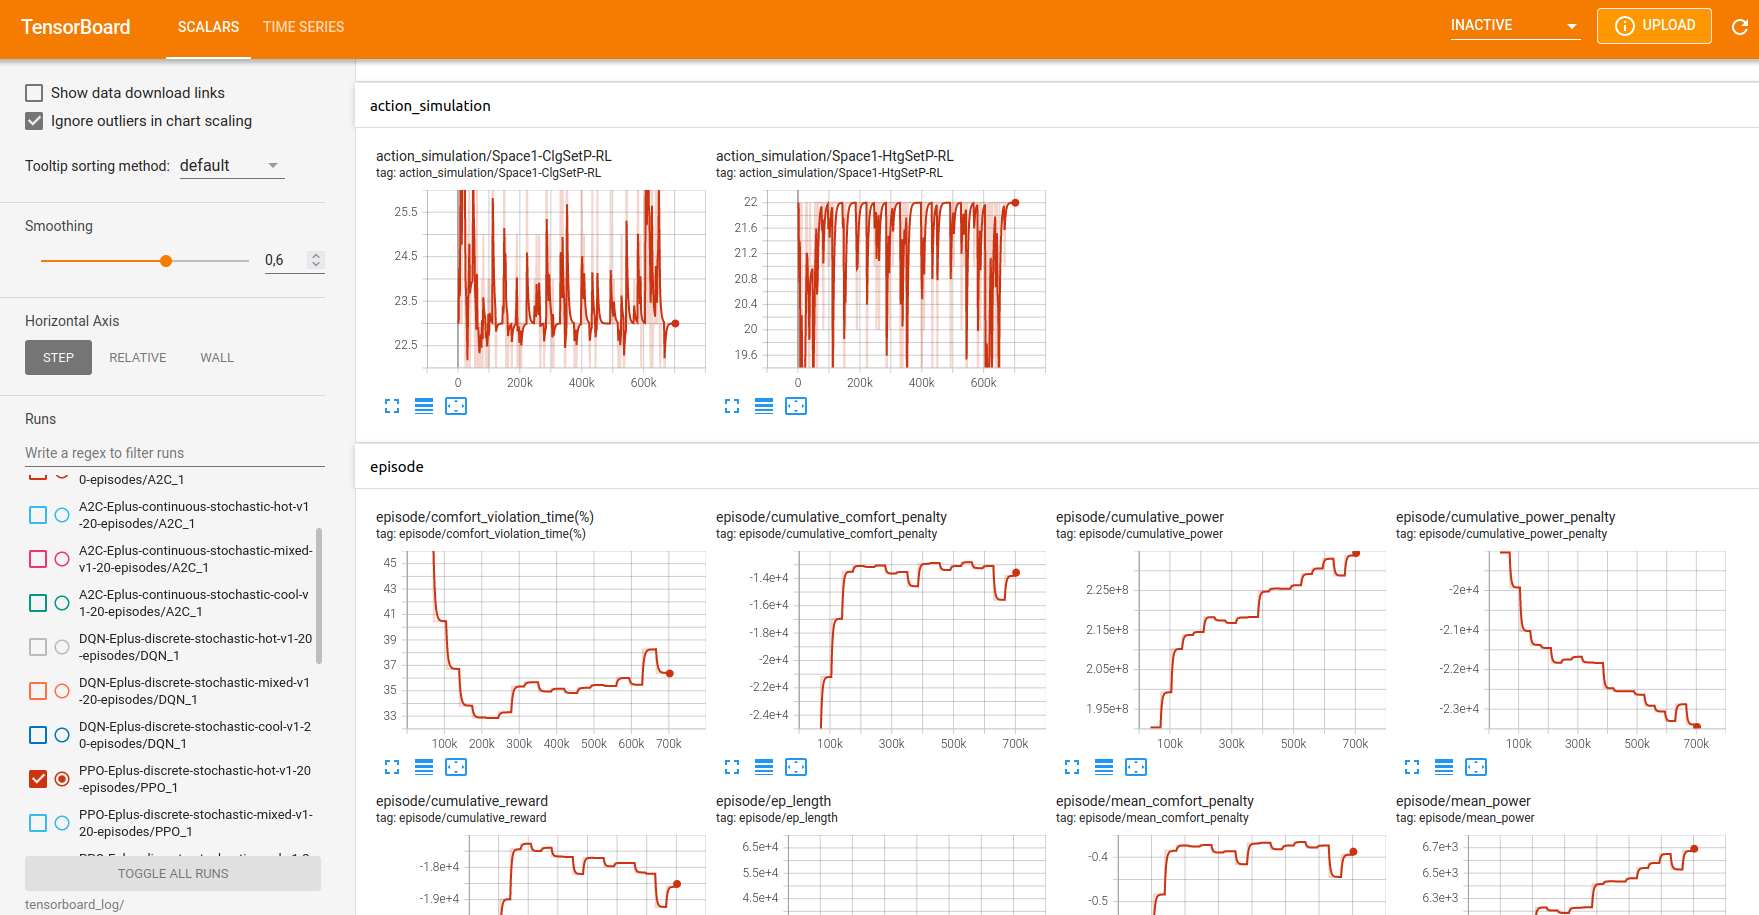
\includegraphics[width=\textwidth]{imagenes/tensorboard.png}
    \caption{Monitorización del entrenamiento mediante TensorBoard}
    \label{fig:tensorboard}
\end{figure}

Finalmente, veamos la información recogida y mostrada por TensorBoard, la cual se divide en los siguientes grupos:

\begin{itemize}
    \item Registro de las acciones empleadas por el agente durante la simulación.
    \item Medidas de rendimiento recopiladas episodio a episodio:
    \begin{itemize}
        \item Porcentaje de tiempo bajo violación de confort, donde la temperatura estuvo fuera de los límites de confort definidos.
        \item Valor medio y suma acumulada de las penalizaciones por confort durante un episodio completo.
        \item Consumo energético total a lo largo de cada episodio.
        \item Valor medio y suma acumulada de las penalizaciones por consumo energético.
        \item Recompensa media y acumulada.
        \item Duración (en \textit{timesteps}) de cada episodio.
    \end{itemize}
    \item Valor de las variables observadas durante la simulación (dependientes del entorno).
    \item Valores normalizados de las variables observadas, en caso de emplearse el \textit{wrapper} de normalización previamente mencionado.
    \item Métricas ofrecidas por Stable Baselines3 relacionadas con cada algoritmo (por ejemplo, la variación del ratio de exploración en DQN).
    \item Tiempo de ejecución.
    \item Información sobre los valores de entrenamiento de las redes neuronales, ofrecida por Stable Baselines3.
    \item Medidas de rendimiento obtenidas en los episodios de evaluación, en caso de utilizar el \textit{callback} \texttt{EvalLoggerCallback} durante el entrenamiento\footnote{Para más información sobre los \textit{callbacks} ofrecidos por Stable Baselines3, véase: \url{https://stable-baselines.readthedocs.io/en/master/guide/callbacks.html}.}. Este \textit{callback} permite evaluar periódicamente el rendimiento del agente entrenado, empleando un entorno de \textit{test} independiente. A su vez, preserva el mejor modelo obtenido hasta el momento en un directorio indicado por el usuario.
\end{itemize}
    
\subsection{Integración con MLflow}

Por último, con el fin de realizar un seguimiento de los experimentos ejecutados y registrar la configuración de los diferentes algoritmos, se decidió emplear \href{https://mlflow.org/}{MLflow}. Se trata de una plataforma \textit{open source} orientada a la gestión del ciclo de vida en proyectos de \textit{machine learning} y ampliamente utilizada en el ámbito del \href{https://ml-ops.org/}{MLOps}. Su uso es similar al de otras herramientas como \href{https://neptune.ai/}{Neptune}, \href{https://www.comet.ml}{Comet}, \href{https://polyaxon.com/}{Polyaxon}, \href{https://valohai.com/}{Valohai}, \href{https://metaflow.org/}{Metaflow} o \href{https://wandb.ai/site}{WandB}. No obstante, a pesar de las numerosas posibilidades existentes, el hecho de ser \textit{open source}, así como su simplicidad y flexibilidad ante las necesidades de este proyecto fueron las principales razones que llevaron a elegir esta herramienta.

Atendiendo a sus principales funcionalidades, MLflow permite registrar experimentos (\textit{runs}) manteniendo un listado personalizable de las configuraciones empleadas en cada ejecución. También permite comparar su desempeño, elaborar gráficos comparativos entre diversas parametrizaciones, así como almacenar, gestionar y desplegar diferentes versiones de los modelos entrenados.

En el marco de este proyecto, MLflow (y, en especial, su módulo \textit{Model Registry}) resultó de especial interés a la hora de mantener un registro estable de los experimentos realizados y sus configuraciones. Cabe destacar que MLflow no es una herramienta exclusivamente orientada a la gestión de modelos de aprendizaje por refuerzo, pero que contó con la suficiente flexibilidad como para cubrir las necesidades de este proyecto. De esta forma, su principal uso consistió en el registro y estudio de los hiperparámetros empleados en el entrenamiento de los modelos de DRL, así como de las métricas de evaluación empleadas, como la recompensa media o el tiempo de entrenamiento.

Desde un punto de vista práctico, simplemente fue necesario especificar qué parámetros y métricas debían ser empleados durante los experimentos para que MLflow se encargase de su registro y monitorización\footnote{Véase el ejemplo en código disponible en la documentación de Energym: \url{https://energym.readthedocs.io/en/latest/pages/deep-reinforcement-learning.html\#how-use}.}.

Finalmente, en la Figura \ref{fig:mlflow} se muestra el listado de ejecuciones registradas en MLflow, correspondientes a los experimentos que abordaremos en el siguiente capítulo.

\begin{figure}
    \centering
    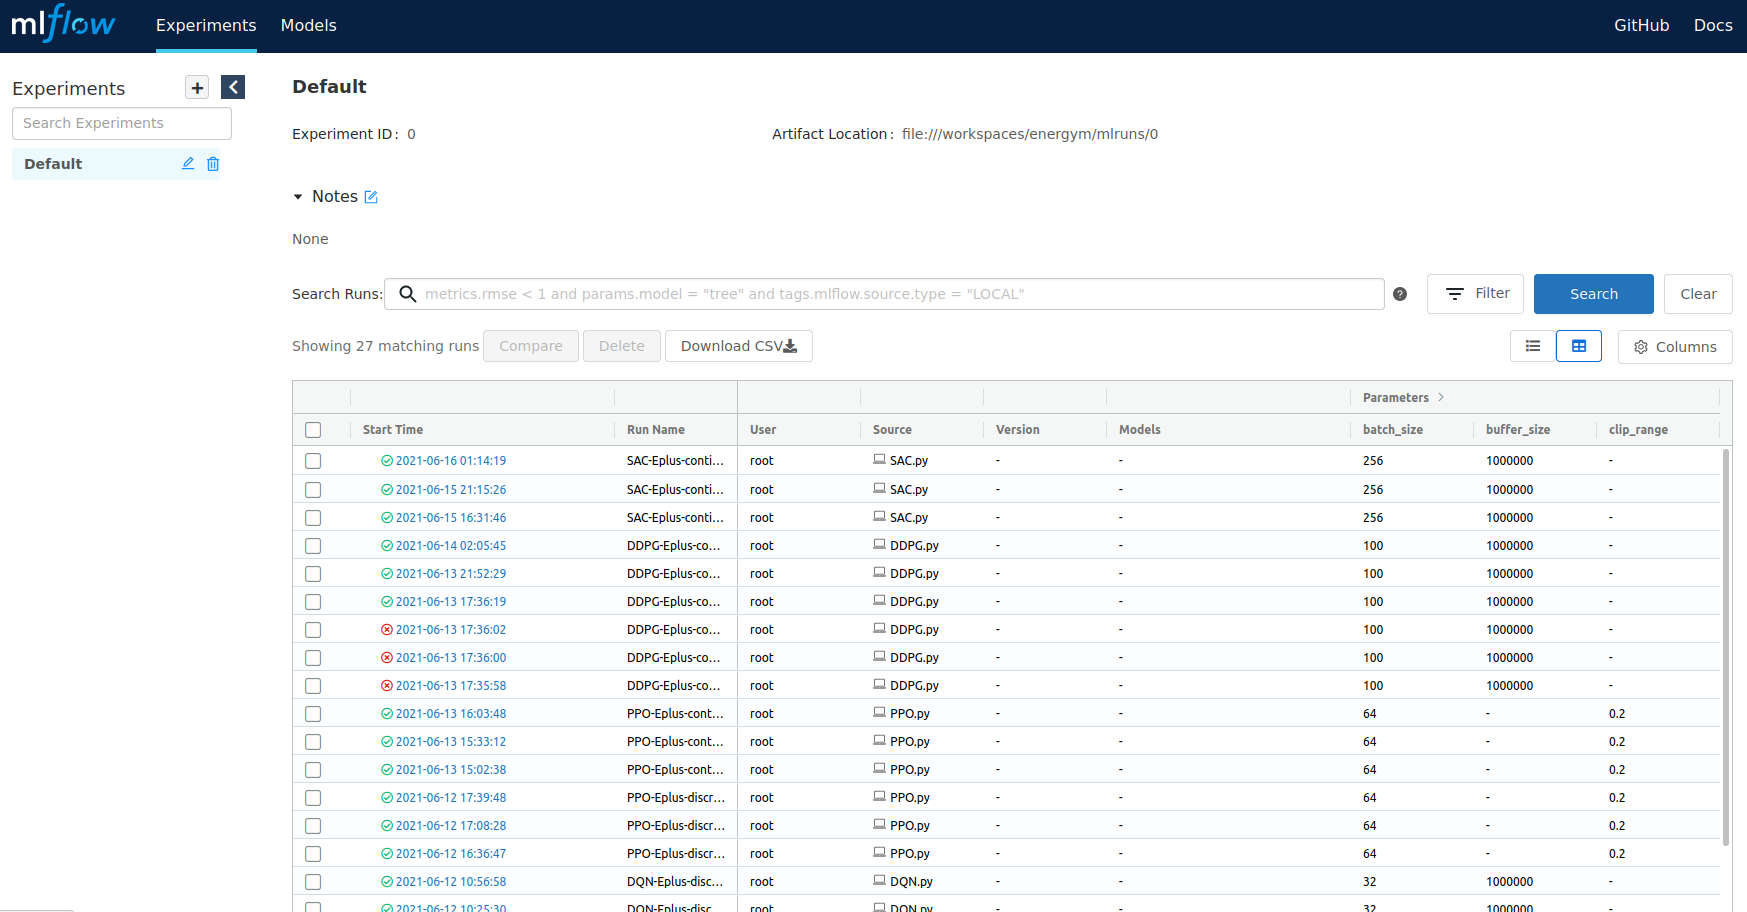
\includegraphics[width=\textwidth]{imagenes/mlflow.png}
    \caption{Experimentos registrados mediante MLflow}
    \label{fig:mlflow}
\end{figure}






\chapter{Experimentación}
\label{ch:4}

En este capítulo se detallará la experimentación realizada con Energym, dando a conocer el rendimiento de diferentes tipos de agentes en múltiples entornos y condiciones, mostrando así las posibilidades que ofrece esta herramienta.

\section{Metodología de experimentación}

Los experimentos llevados a cabo en este capítulo serán los siguientes (ver Figura \ref{fig:metodologia}):

\begin{itemize}
    \item \textbf{Experimentación básica} (sección \ref{sec:evaluacion-agentes}): se entrenarán diferentes agentes disponibles en Stable Baselines3 para posteriormente evaluar su desempeño en espacios de acciones discretos y continuos. Los resultados obtenidos tras dicha evaluación se estudiarán desde diferentes perspectivas, enfatizando en las diferencias entre los resultados obtenidos por un agente basado en reglas convencional y los algoritmos de DRL probados.
    \item \textbf{Experimentación avanzada}: estos experimentos tratarán de profundizar en diferentes aspectos avanzados del problema:
        \begin{itemize}
            \item \textbf{Equilibrio confort-consumo} (sección \ref{sec:conf-con}): se estudiará la influencia de las ponderaciones de confort y consumo en el desempeño de los agentes.
            \item \textbf{Pruebas de robustez} (sección \ref{sec:robustez}): experimentación destinada a estudiar el desempeño de los agentes en entornos para los cuales no han sido entrenados.
            \item \textbf{\textit{Curriculum learning}} (sección \ref{sec:cv-learning}): abordaremos un ejemplo de aplicación de \textit{curriculum learning}, estudiando cómo el aprendizaje progresivo puede ser empleado en este ámbito.
        \end{itemize}
\end{itemize}

\begin{figure}
    \centering
    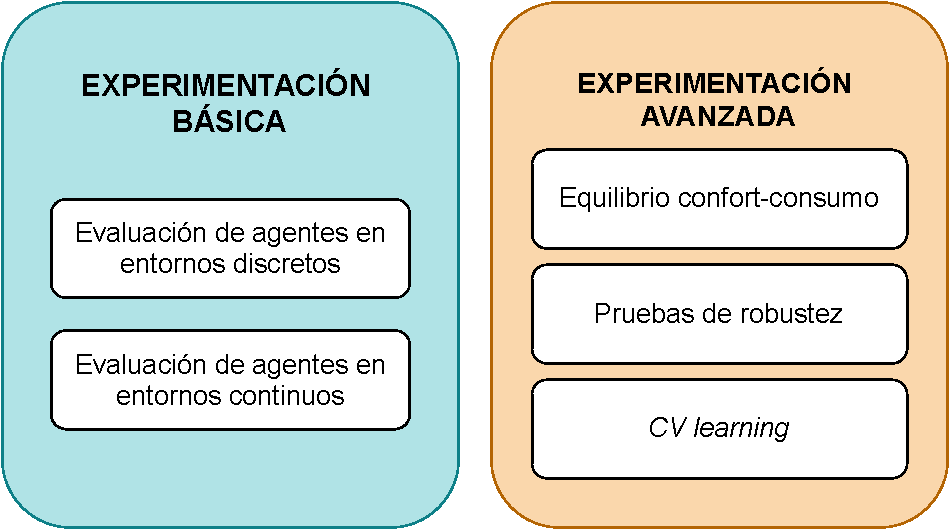
\includegraphics[width=\textwidth]{imagenes/metodologia.pdf}
    \caption{Experimentos realizados empleando Energym}
    \label{fig:metodologia}
\end{figure}

\section{Entorno de simulación}

La experimentación se desarrollará sobre una serie de entornos de simulación, compuestos por un modelo de edificio, diferentes tipos de clima y un conjunto de variables de entrada y salida ofrecidas por el simulador.

\subsection{Edificio}

El modelo de edificio empleado fue \texttt{5ZoneAutoDXVAV}: un edificio de 5 zonas (4 exteriores y 1 interior) climatizadas por medio de un sistema de aire acondicionado de tipo DX (\textit{Direct Expansion Air Conditioning Unit)}\footnote{Para más información sobre este tipo de sistemas, véase: \url{https://www.airconditioning-systems.com/direct-expansion-system.html}}. 

Se trata de un modelo incluido en el repositorio de modelos de ejemplo de EnergyPlus\footnote{El listado completo puede consultarse en: \url{https://github.com/NREL/EnergyPlus/tree/v8.6.0/testfiles}.} y previamente empleado en la literatura relacionada \cite{zhang2018practical}. La experimentación realizada se correspondió con el control de temperatura de una de las estancias.

\subsection{Climas}

Para llevar a cabo la simulación energética de un edificio, es necesario conocer las condiciones climáticas que lo atañen. Dichas condiciones pueden resumirse en un conjunto de datos correspondientes a un período de tiempo y lugar determinados, para posteriormente emplearse en la recreación de ese mismo contexto. 

La clasificación ofrecida por el DOE (Departamento de Energía de Estados Unidos) diferencia entre 19 tipos de clima\footnote{Dicha clasificación puede consultarse en el siguiente enlace: \url{https://www.energycodes.gov/development/commercial/prototype_models}}, desde extremadamente húmedos y cálidos, hasta árticos. Actualmente se encuentran disponibles numerosos repositorios con modelos abiertos de clima destinados a la simulación energética de edificios, como \href{http://climate.onebuilding.org/}{\textit{Climate.OneBuilding}}. En este caso, se utilizaron los tres modelos cuyas temperaturas se muestran en la Figura \ref{fig:weathers}, estos son:

\begin{itemize}
    \item \textbf{\href{https://www.energycodes.gov/sites/default/files/documents/USA_WA_Port.Angeles-William.R.Fairchild.Intl.AP.727885_TMY3.epw}{Clima frío}} (\texttt{cool marine, 5C}): correspondiente al aeropuerto \textit{William R. Fairchild International Airpor} (Washington) entre 1973 y 2005.
    \item \textbf{\href{https://www.energycodes.gov/sites/default/files/documents/USA_NY_New.York-John.F.Kennedy.Intl.AP.744860_TMY3.epw}{Clima templado}} (\texttt{mixed humid, 4A}): correspondiente al aeropuerto \textit{John F. Kennedy International Airport} (Nueva York) entre 1973 y 2005.
    \item \textbf{\href{https://www.energycodes.gov/sites/default/files/documents/USA_AZ_Tucson-Davis-Monthan.AFB.722745_TMY3.epw}{Clima cálido}} (\texttt{hot dry, 2B}): correspondiente a la base aérea \textit{Davis-Monthan Air Force} (Arizona) entre 1973 y 2005.
\end{itemize}

\begin{figure}
    \centering
    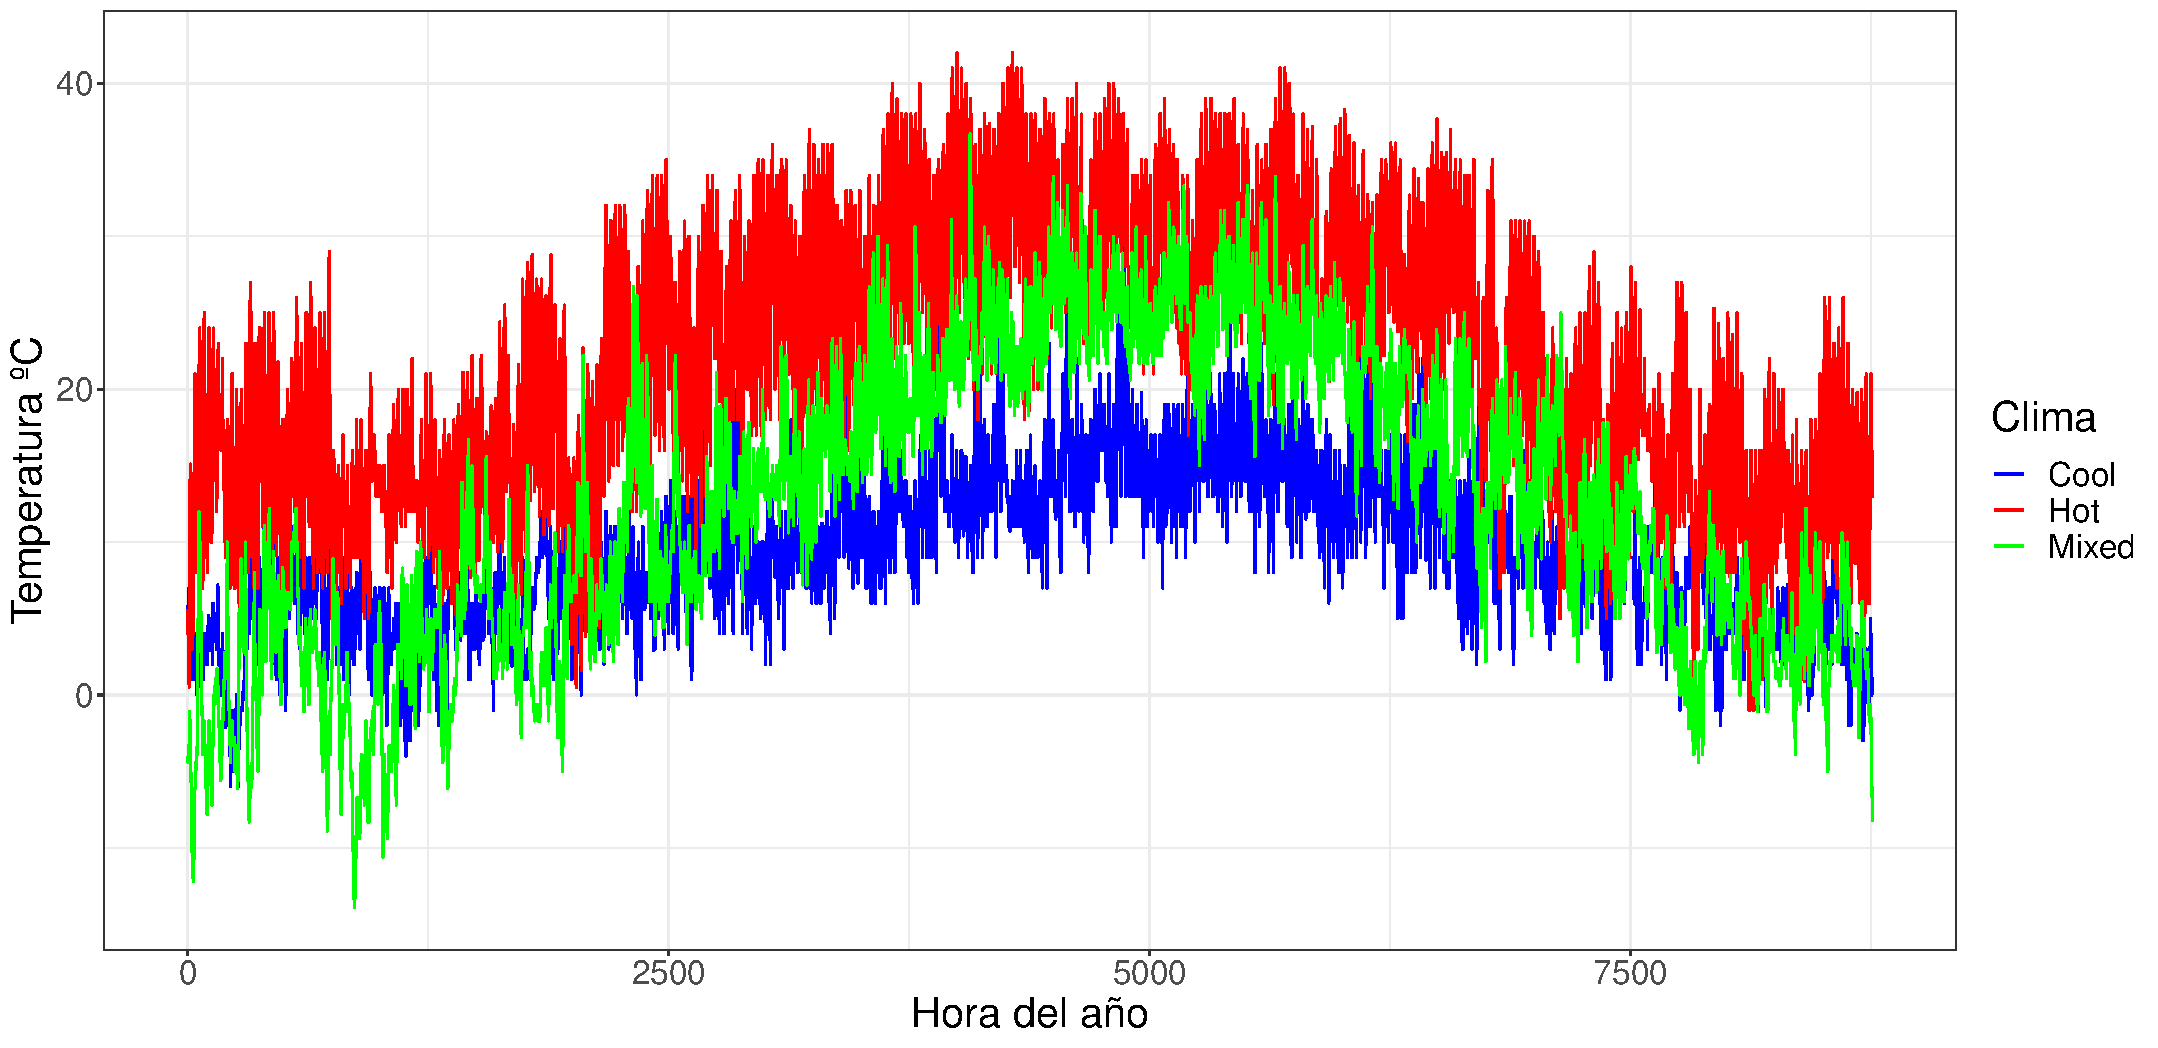
\includegraphics[width=\textwidth]{imagenes/weathers.pdf}
    \caption{Temperaturas (\textit{drybulb}) correspondientes a cada uno de los modelos de clima empleados en la experimentación (se representan los valores medios en cada una de las horas del año)}
    \label{fig:weathers}
\end{figure}

Tal y como se comentó en la sección \ref{sec:entornos}, la inclusión de ruido en estos conjuntos de datos favorece el entrenamiento y permite a los agentes contar con diferentes variaciones de un mismo clima episodio a episodio. Por tanto, los ficheros de clima empleados para realizar las simulaciones fueron una variante de los ya presentados, a los cuales se añadió cierta estocasticidad.

\subsection{Variables}
\label{sec:variables}

Toda simulación cuenta con una serie de variables de entrada (\textit{input variables}) y salida (\textit{output variables}). Mientras que las primeras son modificadas por el agente y tienen una influencia en el entorno, las segundas ofrecen información sobre su situación actual.

En el marco de esta experimentación, un total de 19 variables componen la observación que un agente recibe del entorno\footnote{Véase: \url{https://energym.readthedocs.io/en/latest/pages/environments.html\#observation-action-spaces}}. Estas son:

\begin{itemize}
    \item\textbf{Temperatura seca del aire en el exterior} (\textit{Site Outdoor Air Drybulb Temperature}).
    \item \textbf{Humedad relativa del aire en el exterior} (\textit{Site Outdoor Air Relative Humidity}).
    \item \textbf{Velocidad del viento} (\textit{Site Wind Speed}).
    \item \textbf{Dirección del viento} (\textit{Site Wind Direction}).
    \item \textbf{Radiación solar difusa por área} (\textit{Site Diffuse Solar Radiation Rate per Area }).
    \item \textbf{Radiación solar directa por área} (\textit{Site Diffuse Solar Radiation Rate per Area}).
    \item \textbf{Temperatura de consigna} (\textit{setpoint}) actual para \textbf{calefacción} (\textit{Zone Thermostat Heating Setpoint Temperature}).
    \item \textbf{Temperatura de consigna} (\textit{setpoint}) actual para \textbf{refrigeración} (\textit{Zone Thermostat Cooling Setpoint Temperature}).
    \item \textbf{Temperatura del aire} (\textit{Zone Air Temperature}).
    \item \textbf{Confort de acuerdo a la temperatura radiante media} (\textit{Zone Thermal Comfort Mean Radiant Temperature}).
    \item \textbf{Humedad relativa del aire} (\textit{Zone Air Relative Humidity}).
    \item \textbf{Confort termal de acuerdo al ropaje} (\textit{Zone Thermal Comfort Clothing Value}).
    \item \textbf{Confort termal de acuerdo al modelo Fanger PPD} (\textit{Zone Thermal Comfort Fanger Model PPD}).
    \item \textbf{Número de ocupantes} (\textit{Zone People Occupant Count}).
    \item \textbf{Temperatura del aire de acuerdo al modelo Fanger} (\textit{People Air Temperature}).
    \item \textbf{Demanda energética de dispositivos HVAC} (\textit{Facility Total HVAC Electric Demand Power}).
    \item \textbf{Día} (\textit{Current Day}).
    \item \textbf{Mes} (\textit{Current Month}).
    \item \textbf{Hora} (\textit{Current Hour}).
\end{itemize}

Por otro lado, las variables de entrada modificadas por el agente se corresponden con las ya descritas en la sección \ref{sec:entornos}:

\begin{itemize}
    \item \textbf{\textit{Setpoint} de calefacción }(\textit{Heating Setpoint}).
    \item \textbf{\textit{Setpoint} de refrigeración} (\textit{Cooling Setpoint}).
\end{itemize}

De esta forma, todo agente recibirá como observación el conjunto de variables inicialmente descrito, y actuará en consecuencia modificando los \textit{setpoints} de acuerdo a sus objetivos de consumo y confort. 

\subsection{Métricas de evaluación}
\label{sec:metricas-evaluacion}

Finalmente, evaluaremos el desempeño de los agentes centrándonos en un conjunto métricas derivadas de las variables de salida previamente descritas. Estas métricas, ejemplificadas en la Figura \ref{fig:DDPG-results}, son las siguientes:

\begin{figure}
    \centering
    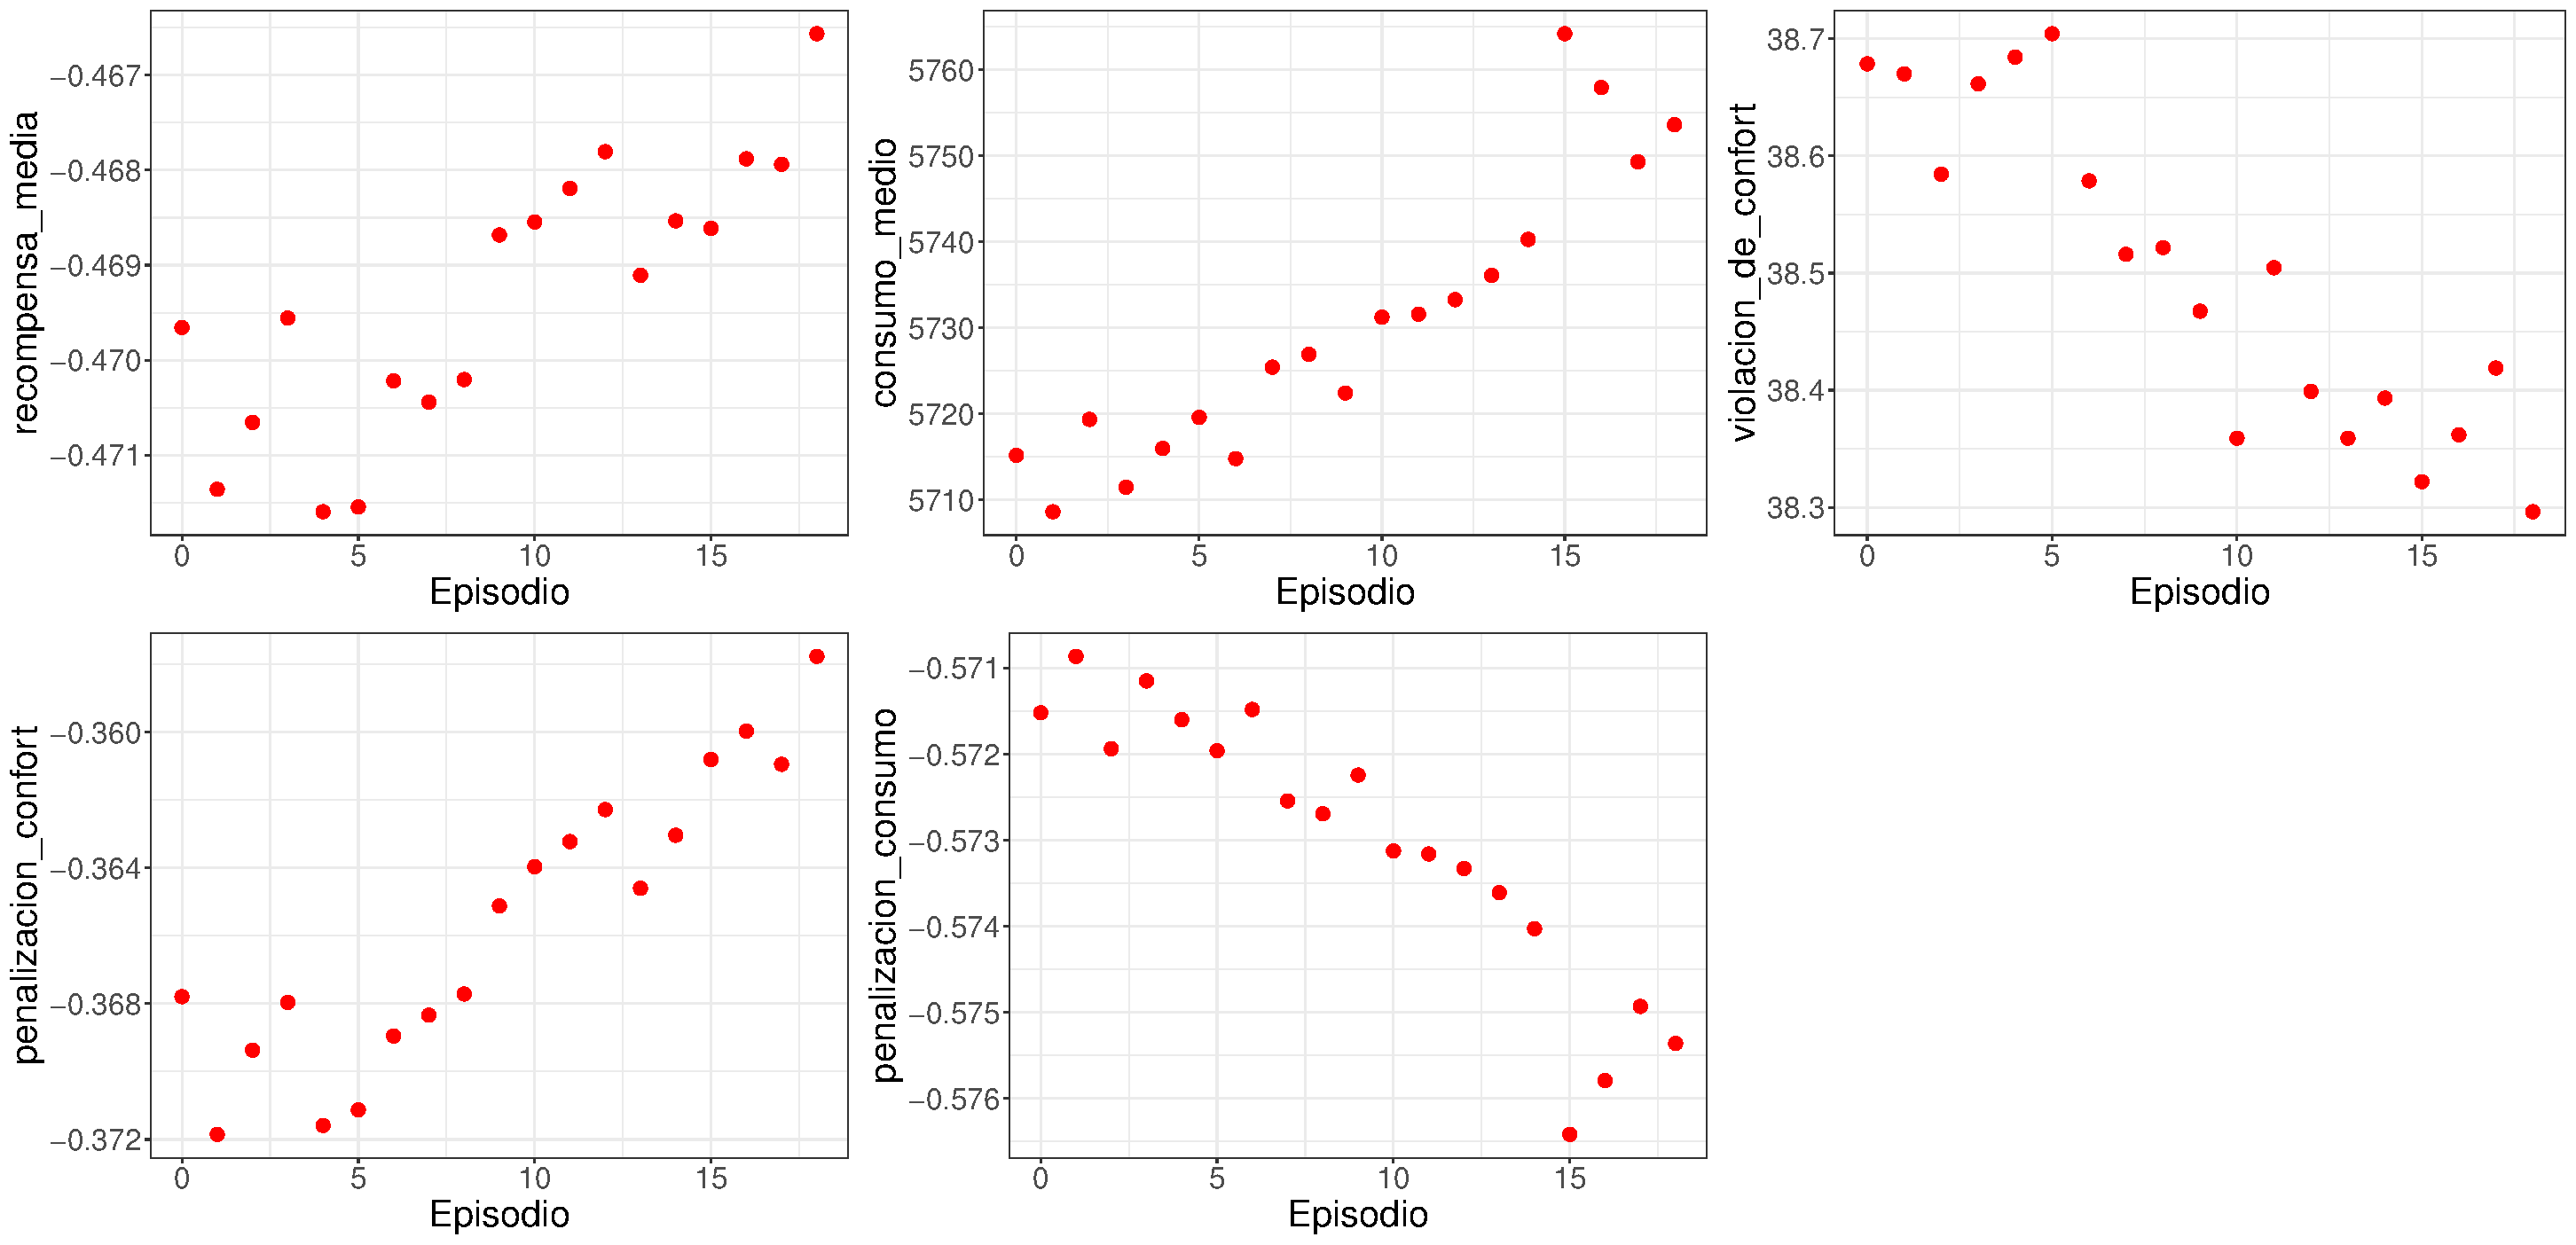
\includegraphics[width=\textwidth]{imagenes/ddpg-cont-mixed-fixed.pdf}
    \caption{Ejemplo de las métricas evaluadas durante la validación de DDPG en el entorno \textit{continuous-stochastic-mixed}}
    \label{fig:DDPG-results}
\end{figure}

\begin{itemize}
    \item \textbf{Recompensa media}: nos indica cómo de bien o mal el agente está garantizando un control eficiente que respete el confort de los ocupantes del edificio y reduzca el consumo.
    
    Recordemos que, tal y como se introdujo en la sección \ref{sec:formulacion}, la función de recompensa empleada por los agentes es la siguiente:
    
    \begin{equation}
        \label{eq:reward-simple}
        r(S_t, A_t) = - w_t \cdot \lambda_c \cdot Confort - (1-w_t) \cdot \lambda_e \cdot Consumo
    \end{equation}
    
     Al estar expresada en términos negativos, buscamos que se mantenga lo más próxima a $0$ posible, o lo que es lo mismo: maximizarla. Así, el cálculo de la recompensa media será igual al promedio de las recompensas medias obtenidas por los agentes en cada episodio.
    
    \item \textbf{Consumo medio}: indica el consumo energético medio a lo largo de la simulación, correspondiente a la variable de salida \textit{Facility Total HVAC Electric Demand Power}. 
    
    Aunque escapa del ámbito de este trabajo profundizar en aspectos referentes al consumo energético, penalización energética, etc., se dota de herramientas a aquellos expertos que deseen hacer un análisis más exhaustivo de estas métricas.
    
    \item \textbf{Violación de confort}: mide el porcentaje de tiempo de un episodio en el que no se ha respetado el intervalo de temperaturas de confort establecidas por el usuario.
    
    \item \textbf{Penalizaciones por confort y consumo} indican el valor medio para cada una de las partes de la recompensa episodio a episodio.
    
    Partiendo de la ecuación \ref{eq:reward-simple}, denominamos ``penalización por consumo'' a: $(1-w_t) \cdot \lambda_e \cdot Consumo$, mientras que $w_t \cdot \lambda_c \cdot Confort$ es la ``penalización por confort''.
\end{itemize}

Una vez presentadas estas métricas, profundizaremos en su análisis para cada uno de los agentes en la sección \ref{sec:results}.

\section{Entrenamiento y evaluación de los agentes}
\label{sec:evaluacion-agentes}

Una vez definidas las condiciones de nuestro experimento, en las siguientes subsecciones evaluaremos los resultados obtenidos tras el entrenamiento y evaluación de los agentes en los entornos discretos y continuos.

El \textit{hardware} empleado para entrenar a los agentes consistió en un equipo \textit{HP Pavilion x360 convertible 14-cd0xxx} equipado con:

\begin{itemize}
    \item Procesador \textit{Intel Core i7-8550U CPU @ 1.80GHz 1.99GHz} de 64 bits.
    \item 12 GB de RAM.
    \item Tarjeta gráfica integrada \textit{Intel UHD Graphics 620}.
    \item Tarjeta gráfica externa \textit{NVIDIA GeForce MX130}.
\end{itemize}

\FloatBarrier
\subsection{Espacio de acciones discreto}

Los algoritmos empleados en los entornos discretos fueron \textbf{DQN}, \textbf{A2C} y \textbf{PPO}. Su entrenamiento fue monitorizado mediante TensorBoard (Figura \ref{fig:train-disc}) y se consideró la siguiente configuración:

\begin{itemize}
    \item Número de episodios de entrenamiento: 20.
    \item Evaluaciones periódicas durante el entrenamiento cada 5 episodios.
    \item Episodios empleados para evaluar durante el entrenamiento: 2.
    \item Hiperparámetros por defecto para todos los algoritmos.
    \item Misma ponderación para confort y consumo ($w_t = 0.5$).
    \item Mismo entorno para entrenamiento y evaluación, con variaciones en el clima episodio a episodio en ambos casos.
\end{itemize}

\begin{figure}
    \centering
    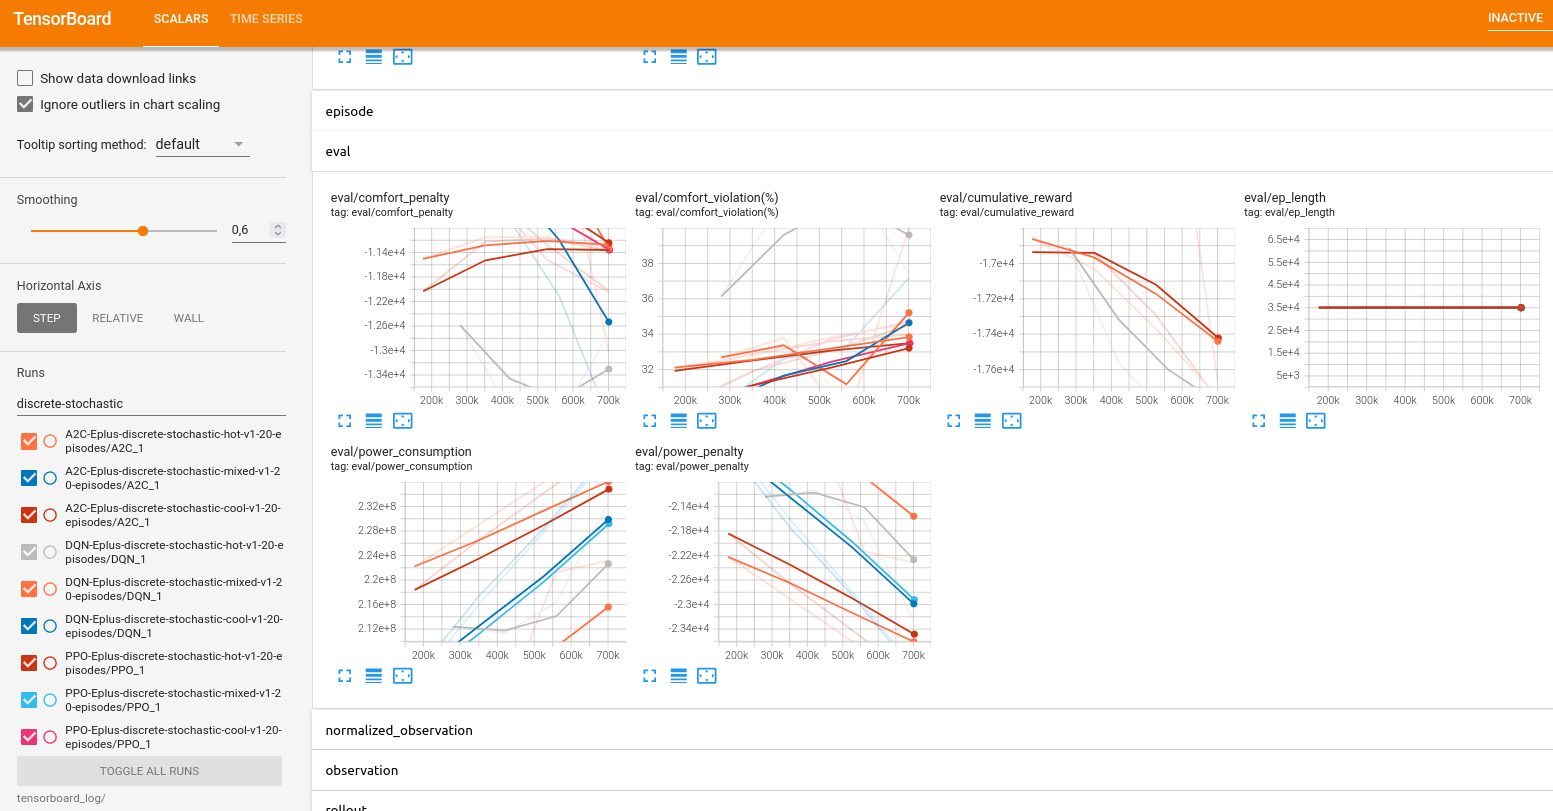
\includegraphics[width=\textwidth]{imagenes/entrenamiento-discretos.png}
    \caption{Proceso de entrenamiento de los entornos discretos monitorizado mediante TensorBoard}
    \label{fig:train-disc}
\end{figure}

Atendiendo a la convergencia de los diferentes modelos, A2C logró converger más rápidamente que el resto, seguido por DQN y PPO. Un ejemplo ilustrativo de dicha convergencia es el que se muestra en la Figura \ref{fig:train-disc-confort}, donde se compara la evolución de la violación de confort para A2C y DQN. En la figura puede verse cómo, a medida que los agentes son entrenados, estos perfeccionan sus políticas, lo que deriva en una reducción de las violaciones de confort y, junto a la reducción del consumo, en una mejora progresiva de las recompensas obtenidas.

\begin{figure}
    \centering
    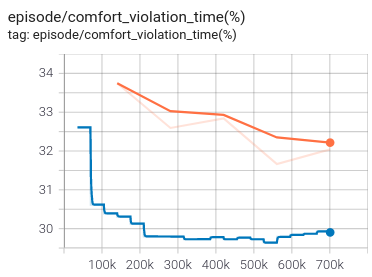
\includegraphics[width=0.7\textwidth]{imagenes/train-disc-violacion-confort.png}
    \caption{Monitorización mediante TensorBoard de la evolución y convergencia de la violación de confort para A2C (azul) y DQN (naranja) en el entorno \textit{discrete-mixed}}
    \label{fig:train-disc-confort}
\end{figure}

Una vez entrenados, se procedió a la validación del mejor modelo obtenido para cada algoritmo de DRL, así como de un agente basado en reglas (RBC) de cara a poder comparar. Dicha validación consistió en la ejecución de cada modelo durante un total de 20 episodios, lo que sirvió para comprobar la generalización y adaptabilidad de los agentes a medida que el ruido sobre el clima se iba acumulando\footnote{Evaluaciones de tal longitud no son comunes en la literatura, siendo 1 ó 2 episodios los empleados normalmente para validar un agente ya entrenado. No obstante, como se ha indicado, una validación mucho más prologada permite conocer la capacidad de generalización de los agentes a medida que las condiciones climáticas se vuelven más extremas.}.

Como se detallará en la sección \ref{sec:results}, se observó un rendimiento significativamente bajo (en comparación con el RBC) en prácticamente la totalidad de los casos, pudiendo deberse este bajo rendimiento a la dependencia entre \textit{setpoints} fríos y calientes y al uso un espacio de acciones quizá demasiado limitado. Esto no fue un problema para los agentes en entornos continuos, donde cada \textit{setpoint} pudo tomar valores de forma independiente.

\FloatBarrier
\subsection{Espacio de acciones continuo}

En el caso de los entornos con espacios de acciones continuos, los algoritmos empleados fueron \textbf{DDPG}, \textbf{PPO}, \textbf{A2C} y \textbf{SAC}. Por otro lado, las condiciones de entrenamiento (ver Figuras \ref{fig:train-cont} y \ref{fig:train-cont-confort}) fueron las mismas que las de los algoritmos en entornos discretos.

\begin{figure}
    \centering
    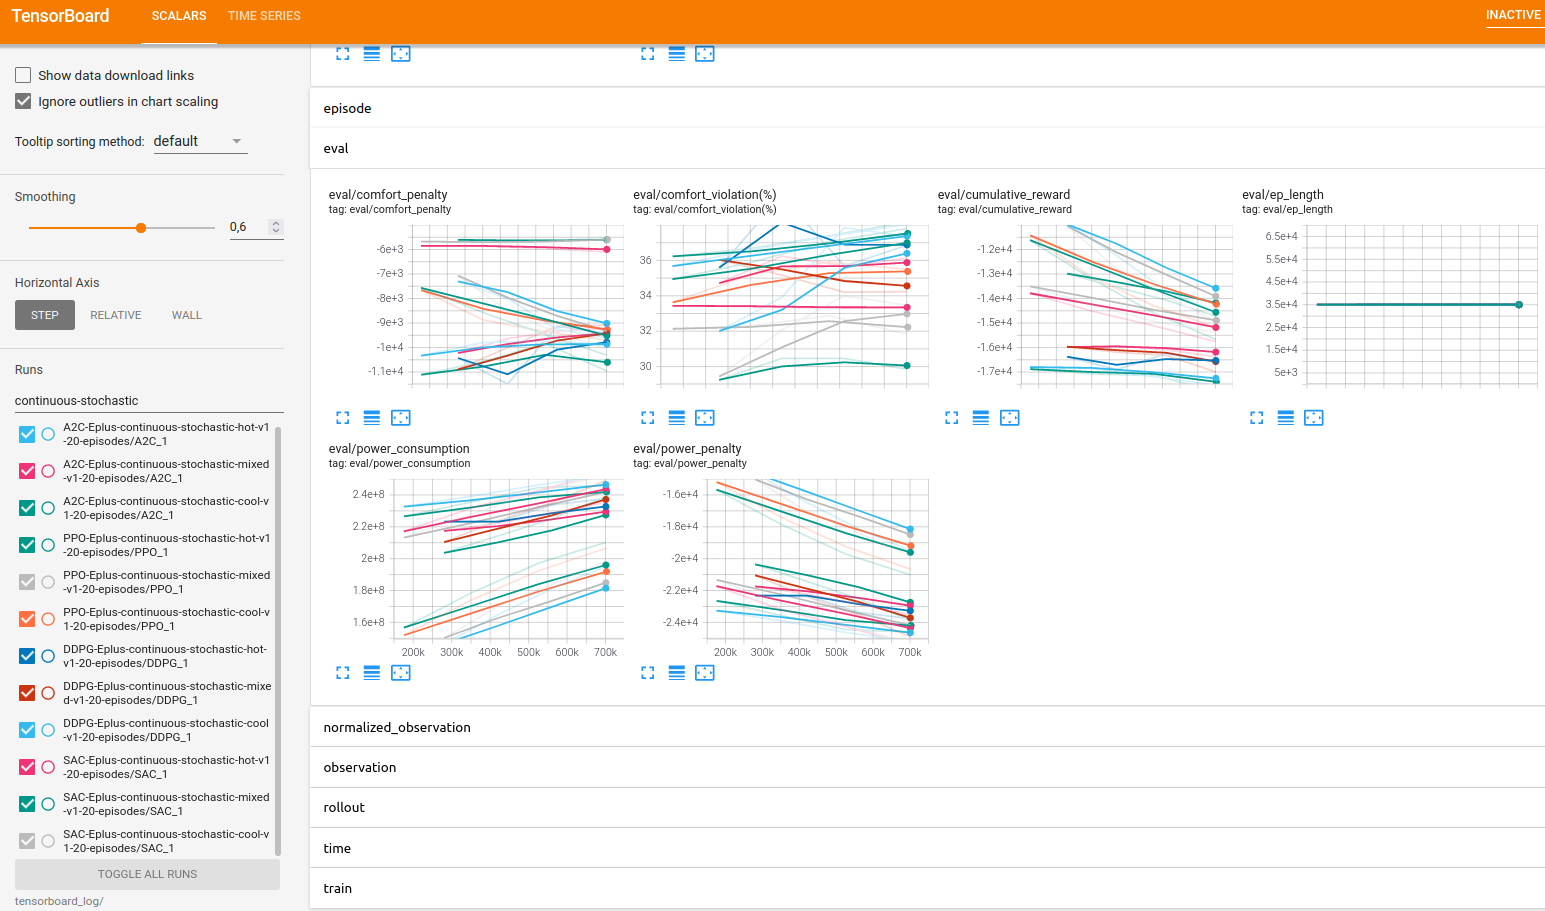
\includegraphics[width=\textwidth]{imagenes/entrenamiento-continuos.png}
    \caption{Proceso de entrenamiento de los entornos continuos monitorizado mediante TensorBoard}
    \label{fig:train-cont}
\end{figure}

\begin{figure}
    \centering
    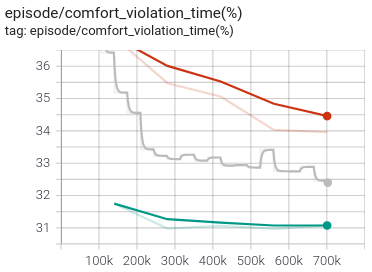
\includegraphics[width=0.7\textwidth]{imagenes/train-cont-confort-violation.png}
    \caption{Monitorización mediante TensorBoard de la evolución y convergencia de la violación de confort para DDPG (rojo), PPO (gris) y SAC (verde) en el entorno \textit{continous-mixed}}
    \label{fig:train-cont-confort}
\end{figure}

Aunque más adelante profundizaremos en los resultados obtenidos, inicialmente se comprobó que:

\begin{itemize}
    \item A2C presenta un comportamiento prácticamente similar a RBC en todos los escenarios.
    \item PPO se comporta de forma similar a A2C y RBC en el entorno templado y ofrece peores resultados para los climas cálido y frío.
    \item DDPG obtiene peores resultados con respecto al resto de algoritmos en entornos templados, pero destaca junto a SAC en los entornos cálido y frío.
    \item SAC presenta los mejores resultados, con un rendimiento generalmente superior al resto (especialmente en el entorno templado), aunque similar al de DDPG en los climas cálido y frío.
\end{itemize}

Un aspecto importante a considerar es cómo la convergencia de los agentes en entornos continuos fue considerablemente más lenta que la de los basados en espacios de acciones discretos. Por lo general, se requiere de un mayor tiempo de entrenamiento para que los algoritmos en entornos continuos alcancen sus mejores resultados.

Finalmente, tanto en los entornos discretos como continuos se observó que un mayor tiempo de entrenamiento supone, a largo plazo, un rendimiento mucho mejor. No obstante, dados los altos requisitos computacionales que supone dicho entrenamiento (con tiempos de entrenamiento para 20 episodios de hasta 3 horas en entornos discretos y 9 horas en los continuos), centraremos nuestra atención en ilustrar los resultados obtenidos para esta prueba limitada a 20 episodios.

\FloatBarrier
\subsection{Resultados}
\label{sec:results}

El entrenamiento de los diferentes agentes, tanto en entornos discretos como continuos, dio lugar a una gran cantidad de datos y gráficas correspondientes a las variables monitorizadas por TensorBoard. Como escapa del ámbito de este trabajo realizar un análisis en profundidad de cada métrica y algoritmo, nos centraremos en estudiar el rendimiento de los agentes desde la perspectiva de las métricas de evaluación previamente presentadas en la sección \ref{sec:metricas-evaluacion}: \textbf{recompensa} (recompensa media), \textbf{consumo} (consumo medio y penalización por consumo) y \textbf{confort} (violación de confort y penalización por confort). 

Así, basándonos en los resultados obtenidos en la validación de los agentes, en la Tabla \ref{tb:best-models} se muestra una perspectiva general de los mejores algoritmos para cada entorno, desde el punto de vista de estas métricas de evaluación.

\begin{table}
    \centering
    \caption{Mejores agentes para diferentes entornos y métricas}
    \label{tb:best-models}
    \resizebox{\textwidth}{!}{%
    \begin{tabular}{cccc}
    \textbf{Entorno} & \textbf{Recompensa} & \textbf{Consumo} & \textbf{Confort} \\ \hline
    \textbf{Disc. hot} & RBC/A2C & DQN & RBC/A2C \\ \hline
    \textbf{Disc. mixed} & RBC & DQN & RBC/A2C \\ \hline
    \textbf{Disc. cool} & RBC/A2C & PPO & RBC/A2C \\ \hline
    \textbf{Cont. hot} & DDPG/SAC & SAC & DDPG \\ \hline
    \textbf{Cont. mixed} & DDPG/SAC & DDPG & SAC \\ \hline
    \textbf{Cont. cool} & SAC & SAC & SAC\\ \hline
    \end{tabular}%
    }
\end{table}

Como se mencionó anteriormente, el rendimiento de los algoritmos en espacios de acciones discretos fue significativamente peor que en los continuos, acercándose al controlador basado en reglas pero sin llegar a superarlo en la mayoría de los casos. Por otro lado, también se enfatizó en el hecho de que los agentes en entornos continuos requieren de un mayor número de episodios para converger en su entrenamiento, al tratarse de espacios de acciones mucho más complejos. Dicha complejidad se debe a que los \textit{setpoints} de calor y frío se ajustan con respecto a un intervalo de valores mucho mayor. De esta forma, estamos ante algoritmos más flexibles, donde no existe ninguna interdependencia entre ambos \textit{setpoints} que pueda afectar al rendimiento, como sí ocurre en los entornos discretos.

La solución al bajo rendimiento de los entornos discretos pasaría por ampliar el número de acciones disponibles, ofreciendo una posibilidad de mapeo mucho mayor, así como por la definición de espacios de acciones multidiscretos. Dichas propuestas están presentes en la sección \ref{sec:trabajo-futuro}, dedicada a aquellos trabajos futuros que puedan derivarse de este proyecto.

Hechas estas aclaraciones, pasemos a analizar cuantitativamente los resultados obtenidos en la \textbf{validación} de los agentes entrenados.

\subsubsection{Consumo energético}

Desde el punto de vista del consumo energético medio en los entornos discretos (Tabla \ref{tb:consumo-disc}), A2C ofreció unos resultados muy similares a los del RBC, sin ofrecer una mejora significativa en ninguno de los tres casos. Por otro lado, PPO logró una mejora del $2.87\%$ en el entorno frío, mientras que DQN redujo el consumo del RBC en los entornos cálido y templado, con disminuciones de consumo del $5.44\%$ y $6.12\%$, respectivamente. No obstante, debe destacarse que estas reducciones en el consumo repercutieron negativamente en el confort, como veremos a la hora de estudiar las recompensas obtenidas.

En el caso de los entornos continuos (Tabla \ref{tb:consumo-cont}), SAC y DDPG lograron mejorar los resultados del RBC con resultados bastante positivos: mientras que SAC logró un consumo un $7.67\%$ y $5.71\%$ inferior en los entornos \textit{hot} (Figura \ref{fig:consumo-cont-hot}) y \textit{mixed}, respectivamente, DDPG obtuvo el menor consumo en el entorno frío con una reducción del $7.45\%$.

\begin{table}
    \centering
    \caption{Consumo medio de los agentes entrenados en entornos discretos a lo largo de 20 episodios de validación}
    \label{tb:consumo-disc}
    \resizebox{0.8\textwidth}{!}{%
    \begin{tabular}{ccccccc}
     & \multicolumn{2}{c}{\textbf{HOT}} & \multicolumn{2}{c}{\textbf{COOL}} & \multicolumn{2}{c}{\textbf{MIXED}} \\ \hline
     & \textit{media} & \textit{desv} & \textit{media} & \textit{desv} & \textit{media} & \textit{desv} \\ \hline
    \textbf{RBC} & 6428 & 171 & 4421 & 507 & 5911 & 223 \\ \hline
    \textbf{A2C} & 6403 & 178 & 4426 & 524 & 5960 & 249 \\ \hline
    \textbf{PPO} & 6278 & 139 & \textbf{4294} & 490 & 5800 & 229 \\ \hline
    \textbf{DQN} & \textbf{6078} & 149 & 4369 & 505 & \textbf{5549} & 238 \\ \hline
    \end{tabular}%
    }
\end{table}

\begin{table}
    \centering
    \caption{Consumo medio de los agentes entrenados en entornos continuos a lo largo de 20 episodios de validación}
    \label{tb:consumo-cont}
    \resizebox{0.8\textwidth}{!}{%
    \begin{tabular}{ccccccc}
     & \multicolumn{2}{c}{\textbf{HOT}} & \multicolumn{2}{c}{\textbf{COOL}} & \multicolumn{2}{c}{\textbf{MIXED}} \\ \hline
     & \textit{media} & \textit{desv} & \textit{media} & \textit{desv} & \textit{media} & \textit{desv} \\ \hline
    \textbf{RBC} & 6674 & 164 & 4612 & 486 & 6220 & 249 \\ \hline
    \textbf{A2C} & 6664 & 160 & 4630 & 522 & 6223 & 267 \\ \hline
    \textbf{PPO} & 6326 & 122 & 4462 & 486 & 6146 & 260 \\ \hline
    \textbf{DDPG} & 6371 & 132 & \textbf{4268} & 465 & 6119 & 234 \\ \hline
    \textbf{SAC} & \textbf{6162} & 122 & 4359 & 514 & \textbf{5865} & 239 \\ \hline
    \end{tabular}%
    }
\end{table}

\begin{figure}
    \centering
    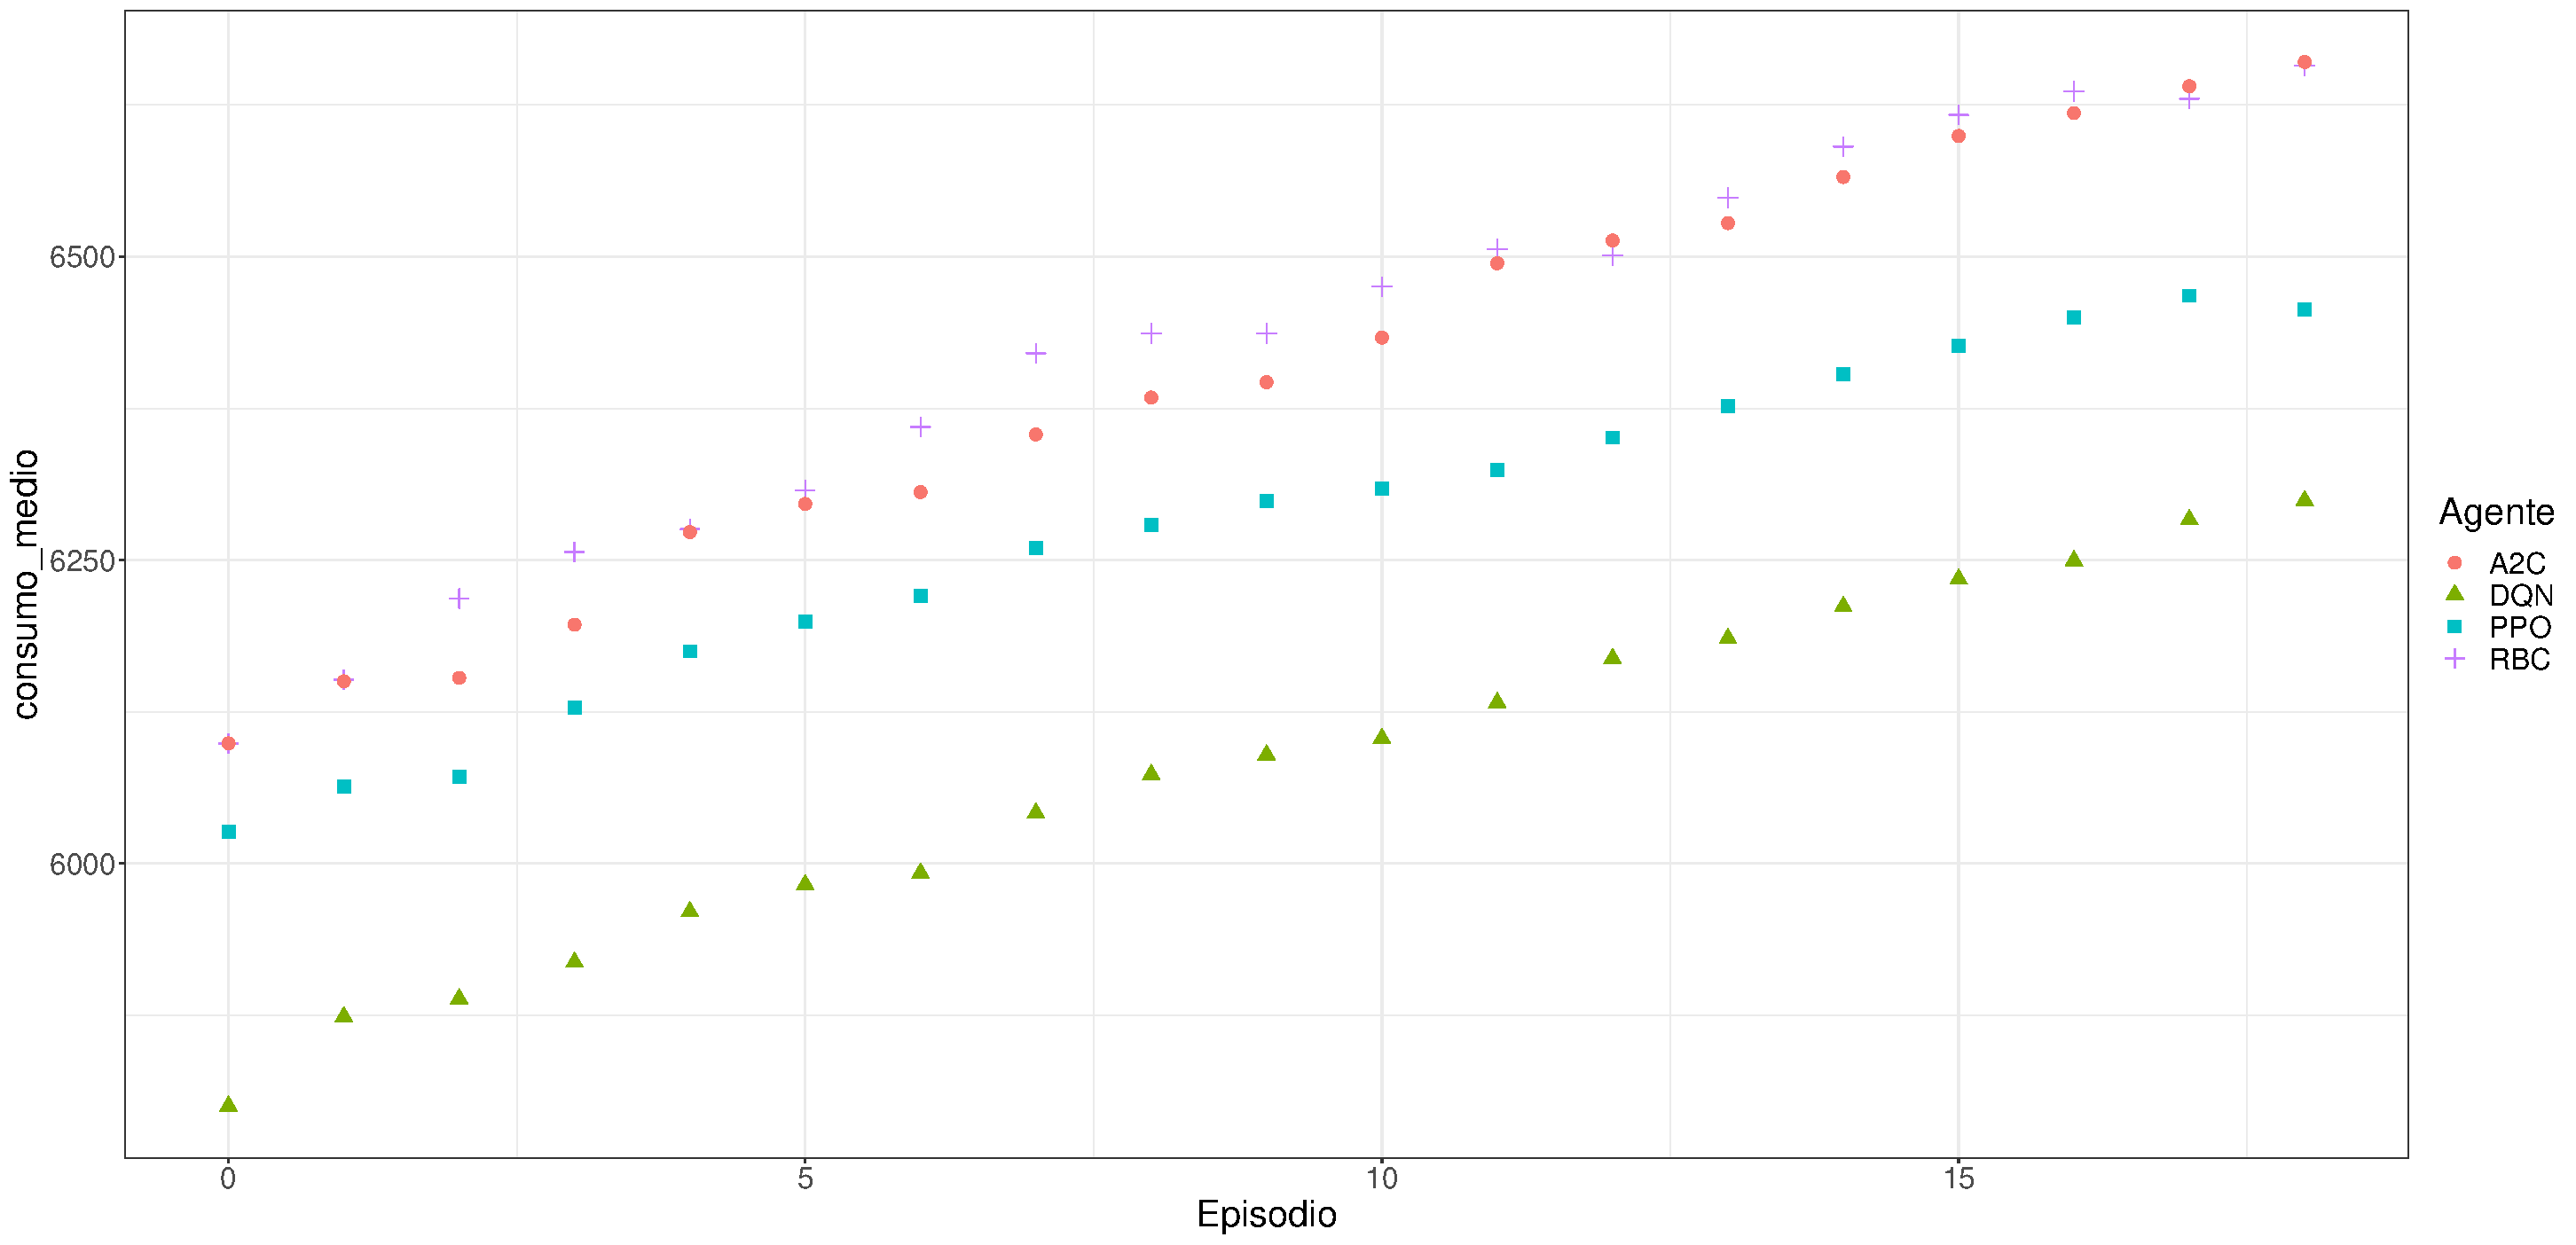
\includegraphics[width=\textwidth]{imagenes/consumo-disc-hot.pdf}
    \caption{Ejemplo del consumo medio obtenido en la validación de los agentes entrenados en el entorno \textit{discrete-stochastic-hot}}
    \label{fig:consumo-disc-hot}
\end{figure}

\begin{figure}
    \centering
    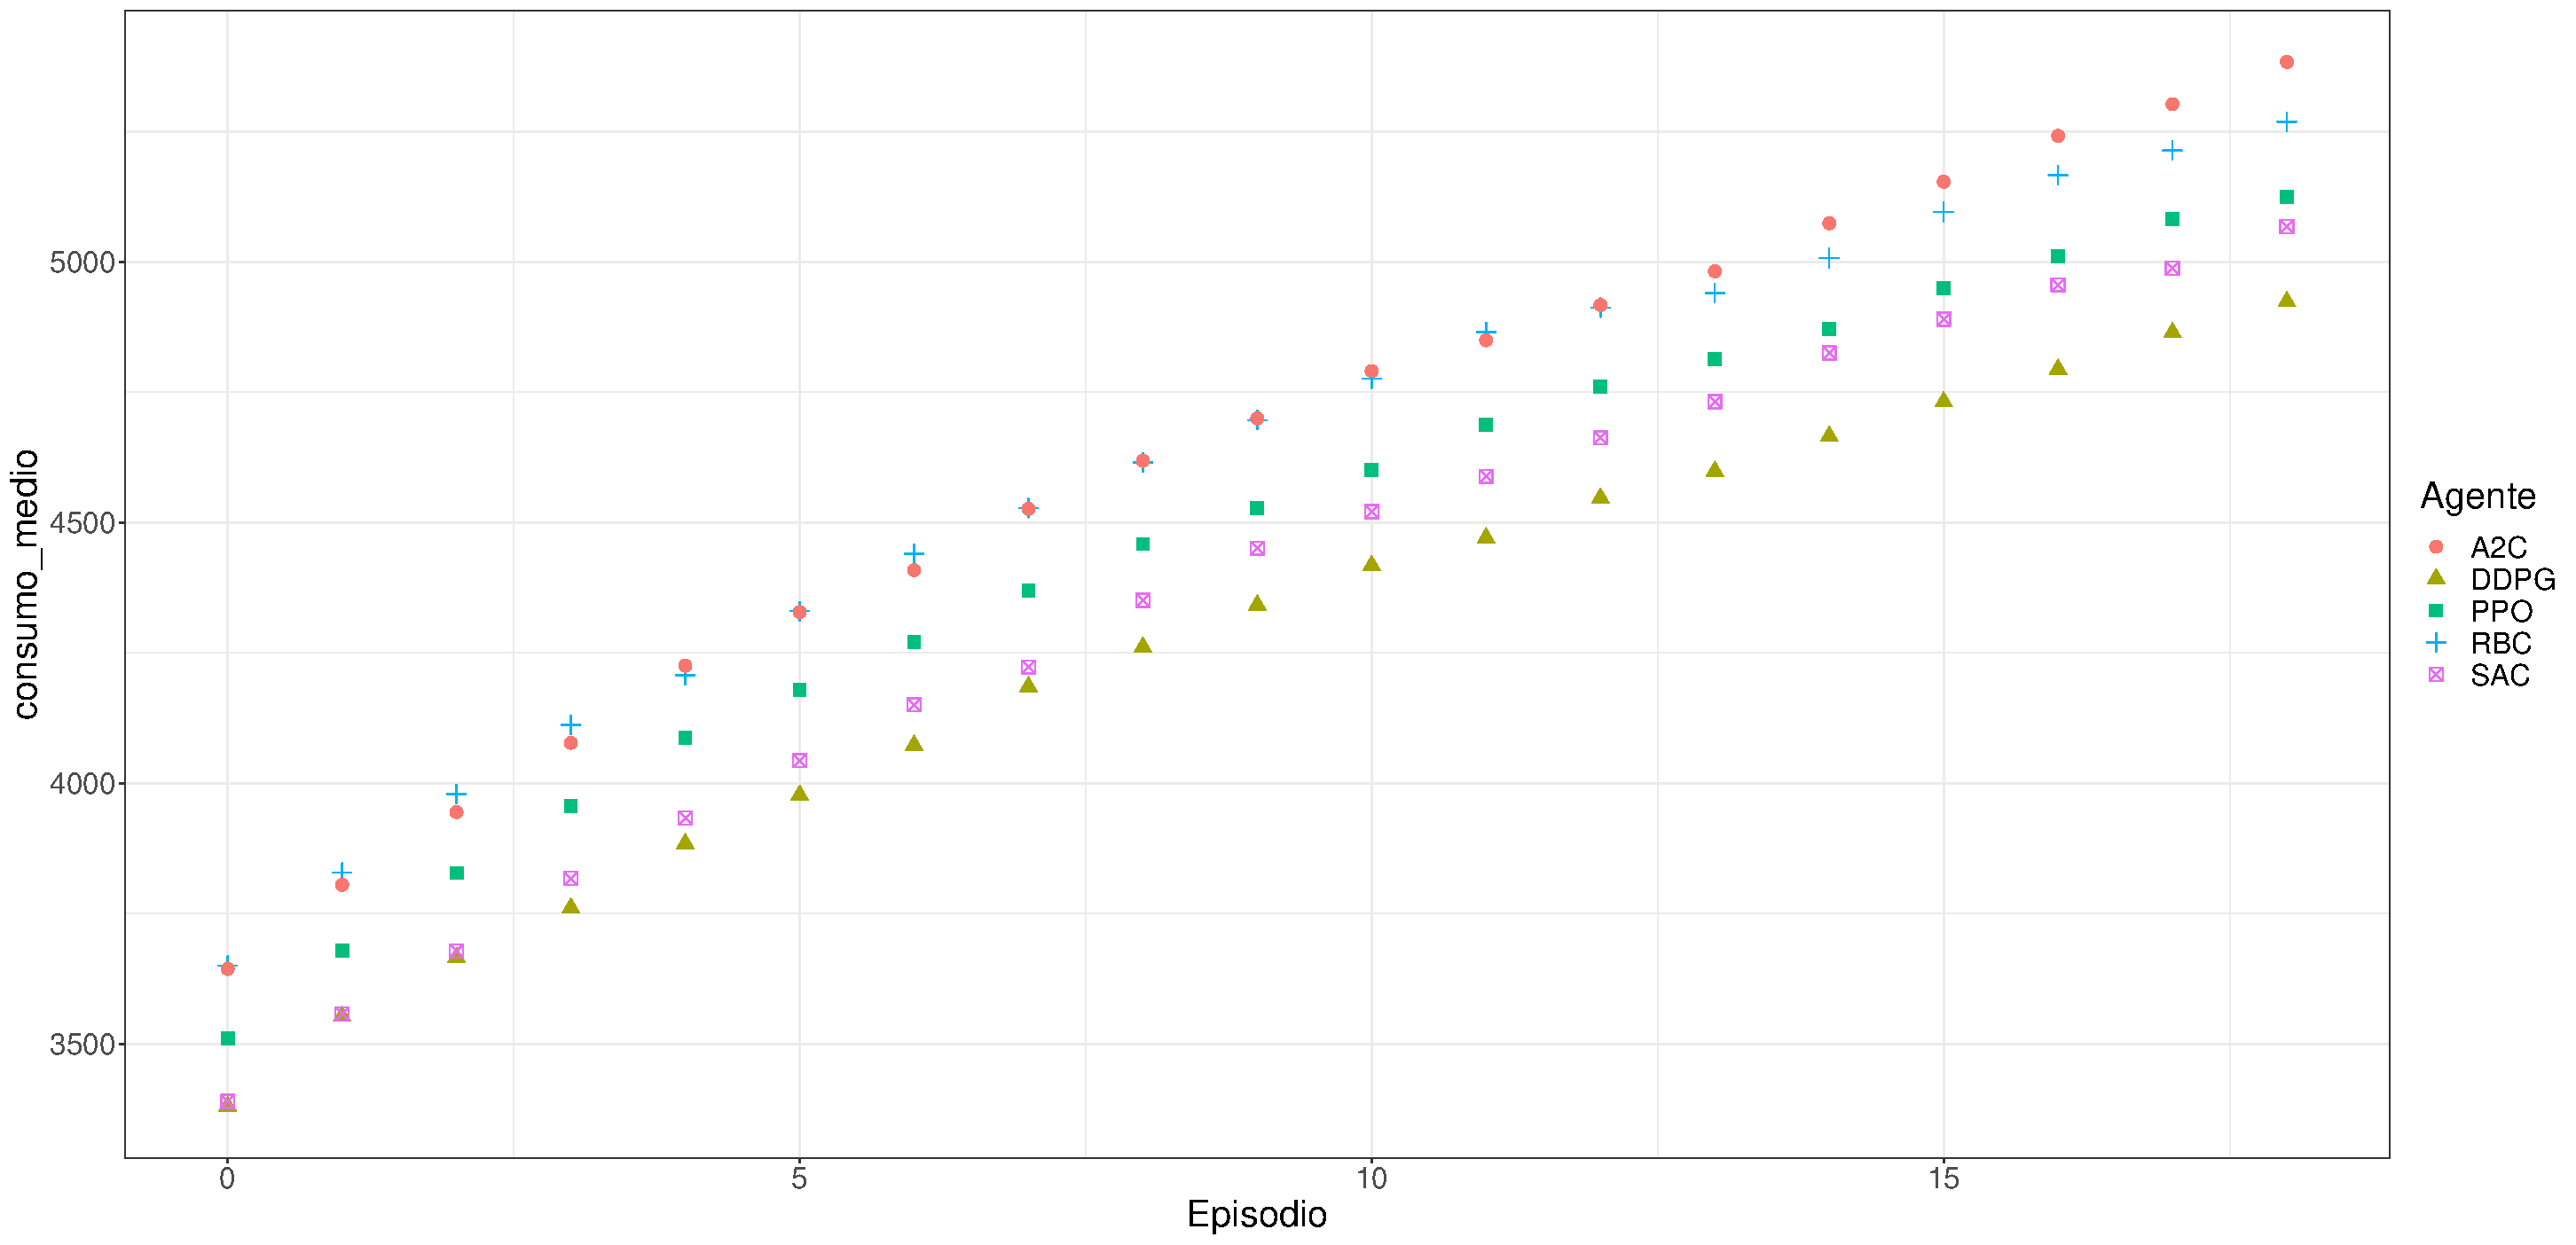
\includegraphics[width=\textwidth]{imagenes/consumo-cont-hot.pdf}
    \caption{Ejemplo del consumo medio obtenido en la validación de los agentes entrenados en el entorno \textit{continuous-stochastic-hot}}
    \label{fig:consumo-cont-hot}
\end{figure}

Finalmente, nótese cómo, tanto en los entornos discretos como continuos, el consumo medio representado en las Figuras \ref{fig:consumo-disc-hot} y \ref{fig:consumo-cont-hot} es creciente debido a la acumulación de ruido en el clima a lo largo del tiempo, lo que dificulta la optimización del consumo energético.

\subsubsection{Confort}

Tomando como referencia el porcentaje de tiempo bajo violación de confort en los entornos discretos, RBC ($32.5\%$) y A2C ($32.6\%$) ofrecieron un desempeño similar para el clima cálido. En el clima templado, los porcentajes fueron del $29.9\%$ y $30\%$, respectivamente, mientras que en el frío, RBC logró un $30.4\%$, A2C un $30.2\%$ y DQN un $31.5\%$. Así, atendiendo a los resultados de la Tabla \ref{tb:confort-disc}, ningún algoritmo de DRL logró mejorar significativamente los resultados del RBC.

Desde la perspectiva de los entornos continuos, se lograron resultados más positivos (ver Tabla \ref{tb:confort-cont}). Frente al bajo rendimiento de A2C y PPO, DDPG logró reducir en un $2.6\%$ la violación de confort con respecto al RBC en clima cálido, mientras que SAC consiguió reducciones del $4.1\%$ y $0.9\%$ en los entornos frío y templado (Figura \ref{fig:confort-cont-mixed}), respectivamente. Aunque no se trata de grandes reducciones en la violación de confort, en la siguiente sección veremos cómo, en combinación con la reducción del consumo, estas se tradujeron en un considerable aumento de las recompensas obtenidas.

\begin{table}
    \centering
    \caption{Violación de confort media de los agentes entrenados en entornos discretos a lo largo de 20 episodios de validación}
    \label{tb:confort-disc}
    \resizebox{0.8\textwidth}{!}{%
    \begin{tabular}{ccccccc}
     & \multicolumn{2}{c}{\textbf{HOT}} & \multicolumn{2}{c}{\textbf{COOL}} & \multicolumn{2}{c}{\textbf{MIXED}} \\ \hline
     & \textit{media} & \textit{desv} & \textit{media} & \textit{desv} & \textit{media} & \textit{desv} \\ \hline
    \textbf{RBC} & \textbf{32.5} & .942 & 30.4 & 1.5 & \textbf{29.9} & .296 \\ \hline
    \textbf{A2C} & 32.6 & .882 & \textbf{30.2} & 1.46 & 30 & .225 \\ \hline
    \textbf{PPO} & 33.9 & .778 & 35.4 & 1.48 & 32.1 & .313 \\ \hline
    \textbf{DQN} & 36.9 & 1.1 & 31.5 & 1.26 & 33.6 & .479 \\ \hline
    \end{tabular}%
    }
\end{table}

\begin{table}
    \centering
    \caption{Violación de confort media de los agentes entrenados en entornos continuos a lo largo de 20 episodios de validación}
    \label{tb:confort-cont}
    \resizebox{0.8\textwidth}{!}{%
    \begin{tabular}{ccccccc}
     & \multicolumn{2}{c}{\textbf{HOT}} & \multicolumn{2}{c}{\textbf{COOL}} & \multicolumn{2}{c}{\textbf{MIXED}} \\ \hline
     & \textit{media} & \textit{desv} & \textit{media} & \textit{desv} & \textit{media} & \textit{desv} \\ \hline
    \textbf{RBC} & 35.9 & .705 & 35.1 & .7 & 33.5 & .064 \\ \hline
    \textbf{A2C} & 36.1 & .675 & 35.1 & .701 & 33.6 & .038 \\ \hline
    \textbf{PPO} & 37.5 & .557 & 34.9 & .933 & 33.6 & .549 \\ \hline
    \textbf{DDPG} & \textbf{33.3} & .944 & 32.9 & 1.55 & 36 & 1.06 \\ \hline
    \textbf{SAC} & 35.7 & .843 & \textbf{31} & 1.29 & \textbf{32.6} & .336 \\ \hline
    \end{tabular}%
    }
\end{table}

\begin{figure}
    \centering
    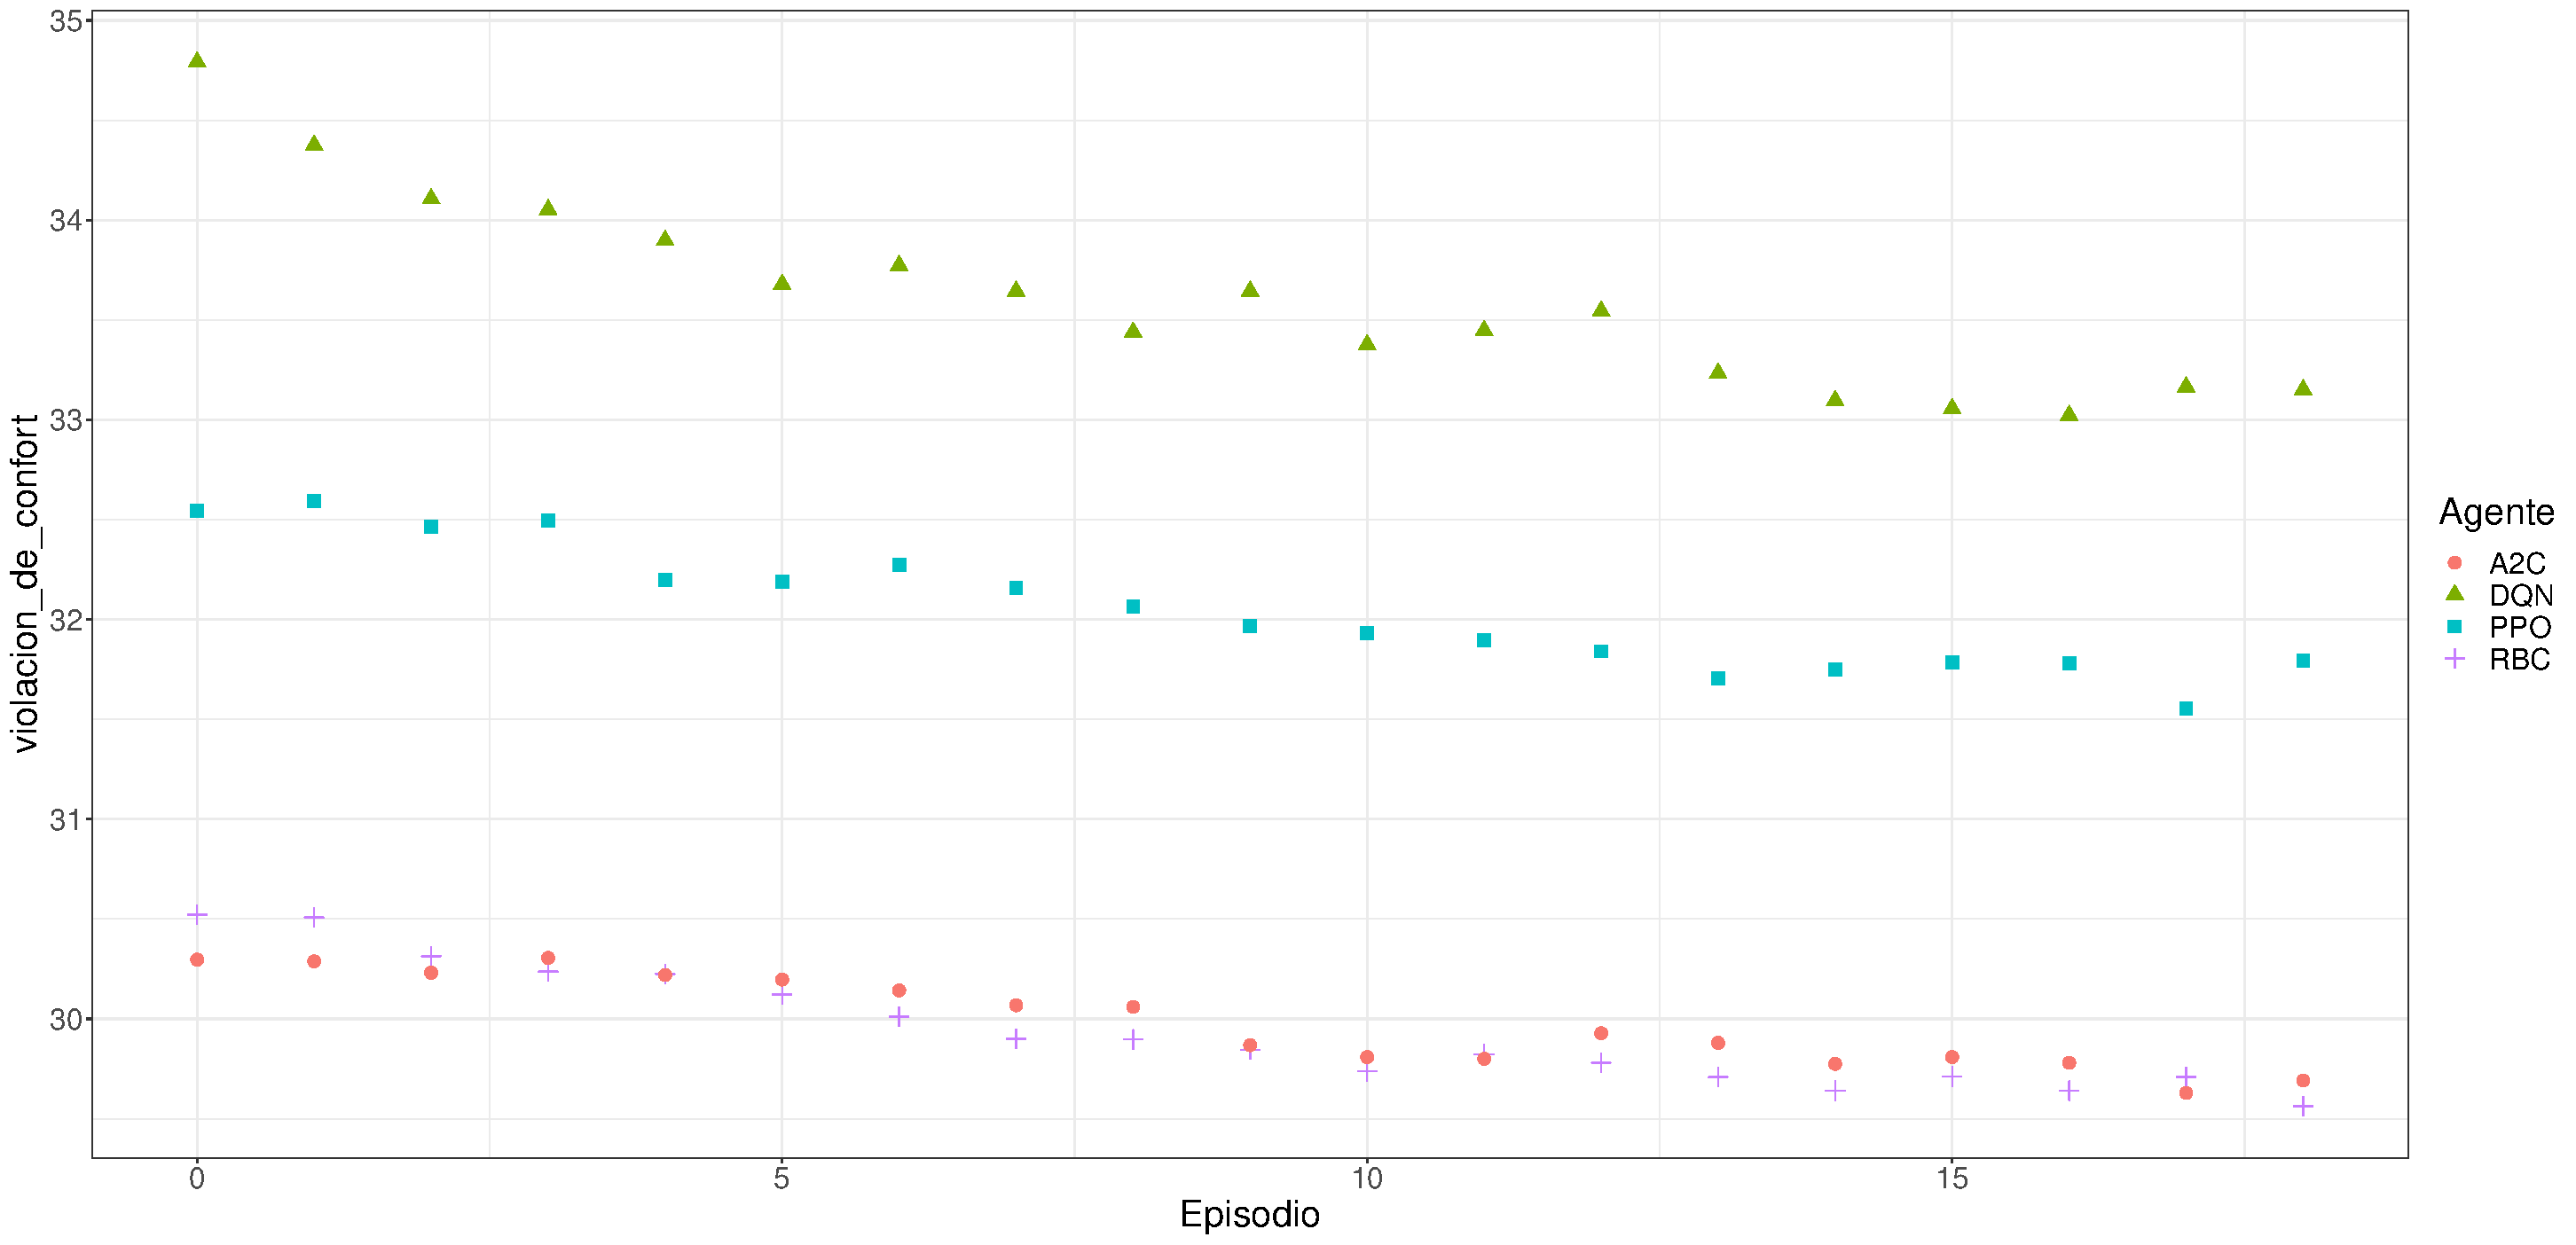
\includegraphics[width=\textwidth]{imagenes/confort-disc-mixed.pdf}
    \caption{Ejemplo de la violación de confort obtenida en la validación de los agentes entrenados en el entorno \textit{discrete-stochastic-mixed}}
    \label{fig:confort-disc-mixed}
\end{figure}

\begin{figure}
    \centering
    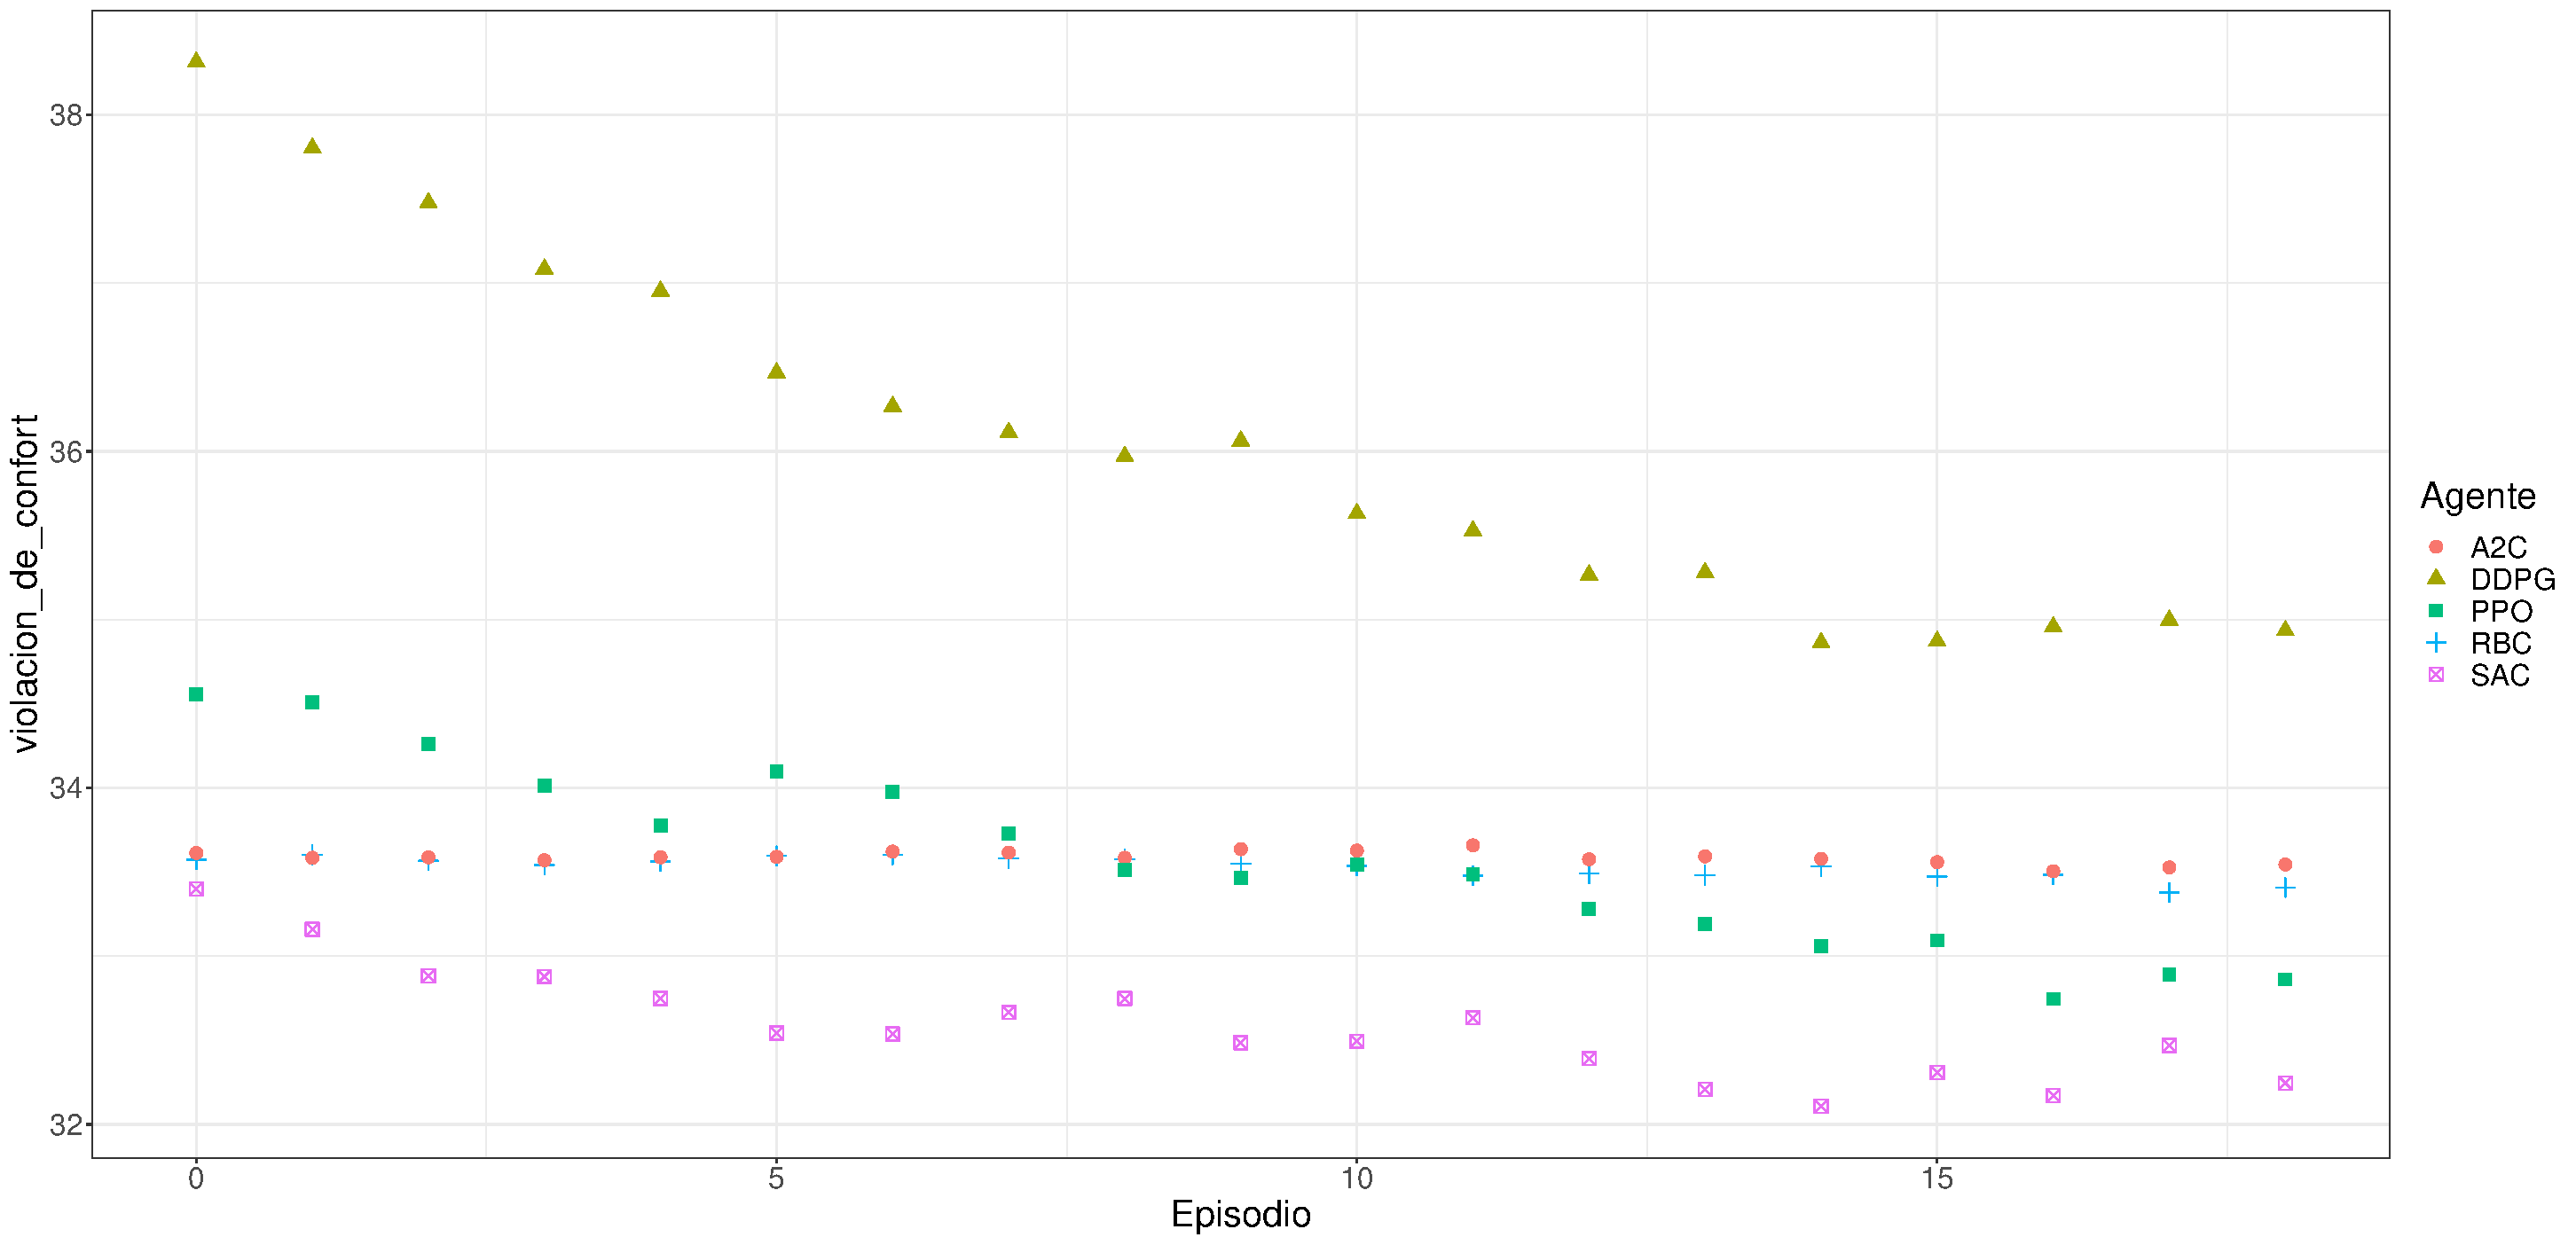
\includegraphics[width=\textwidth]{imagenes/confort-cont-mixed.pdf}
    \caption{Ejemplo de la violación de confort obtenida en la validación de los agentes entrenados en el entorno \textit{continuous-stochastic-mixed}}
    \label{fig:confort-cont-mixed}
\end{figure}

Por último, al igual que en el caso del consumo energético, en las Figuras \ref{fig:confort-disc-mixed} y \ref{fig:confort-cont-mixed} se aprecia cómo los porcentajes de violación de confort empeoran a medida que el clima del entorno cuenta con un mayor ruido acumulado.

\subsubsection{Recompensa}

Finalmente, abordemos el equilibrio entre la minimización del consumo y la maximización del confort, el cual queda reflejado en la función de recompensa empleada. 

En los entornos discretos, A2C y RBC lograron resultados similares, sin apenas variación en sus recompensas medias y superando a las de PPO y DQN en todos los climas (ver Tabla \ref{tb:disc-stats}).

Por otro lado, los resultados más llamativos se dieron en los entornos continuos. En el clima cálido (Figura \ref{fig:recompensa-cont-hot}), las mejoras que SAC y DDPG supusieron frente al RBC fueron del $5.41\%$, mientras que SAC logró superar al RBC en los climas frío y templado con mejoras del $4.73\%$ y $4.71\%$, respectivamente. Estos resultados quedan resumidos en la Tabla \ref{tb:cont-stats}.

En base a estos resultados, se observa que los agentes de DRL en entornos discretos no lograron superar el rendimiento de un RBC. Por el contrario, DDPG y SAC demostraron garantizar un mayor confort y un menor consumo energético que un controlador basado en reglas convencional.

\begin{table}
    \centering
    \caption{Recompensas medias obtenidas por los agentes entrenados en entornos discretos a lo largo de 20 episodios de validación}
    \label{tb:disc-stats}
    \resizebox{0.8\textwidth}{!}{%
    \begin{tabular}{ccccccc}
     & \multicolumn{2}{c}{\textbf{HOT}} & \multicolumn{2}{c}{\textbf{COOL}} & \multicolumn{2}{c}{\textbf{MIXED}} \\ \hline
     & \textit{media} & \textit{desv} & \textit{media} & \textit{desv} & \textit{media} & \textit{desv} \\ \hline
    \textbf{RBC} & \textbf{-.485} & .004 & -.355 & .038 & \textbf{-.422} & .01 \\ \hline
    \textbf{A2C} & -.486 & .005 & \textbf{-.354} & .04 & -.424 & .011 \\ \hline
    \textbf{PPO} & -.502 & .004 & -.394 & .04 & -.436 & .001 \\ \hline
    \textbf{DQN} & -.493 & .004 & -.362 & .038 & -.44 & .008 \\ \hline
    \end{tabular}%
    }
\end{table}

\begin{table}
    \centering
    \caption{Recompensas medias obtenidas por los agentes entrenados en entornos continuos a lo largo de 20 episodios de validación}
    \label{tb:cont-stats}
    \resizebox{0.8\textwidth}{!}{%
    \begin{tabular}{ccccccc}
     & \multicolumn{2}{c}{\textbf{HOT}} & \multicolumn{2}{c}{\textbf{COOL}} & \multicolumn{2}{c}{\textbf{MIXED}} \\ \hline
     & \textit{media} & \textit{desv} & \textit{media} & \textit{desv} & \textit{media} & \textit{desv} \\ \hline
    \textbf{RBC} & -.481 & .003 & -.338 & .036 & -.403 & .013 \\ \hline
    \textbf{A2C} & -.479 & .003 & -.341 & .04 & -.403 & .013 \\ \hline
    \textbf{PPO} & -.496 & .002 & -.351 & .039 & -.403 & .011 \\ \hline
    \textbf{DDPG} & \textbf{-.455} & .002 & -.323 & .041 & -.461 & .004 \\ \hline
    \textbf{SAC} & \textbf{-.455} & .002 & \textbf{-.322} & .042 & \textbf{-.384} & .011 \\ \hline
    \end{tabular}%
    }
\end{table}

\begin{figure}
    \centering
    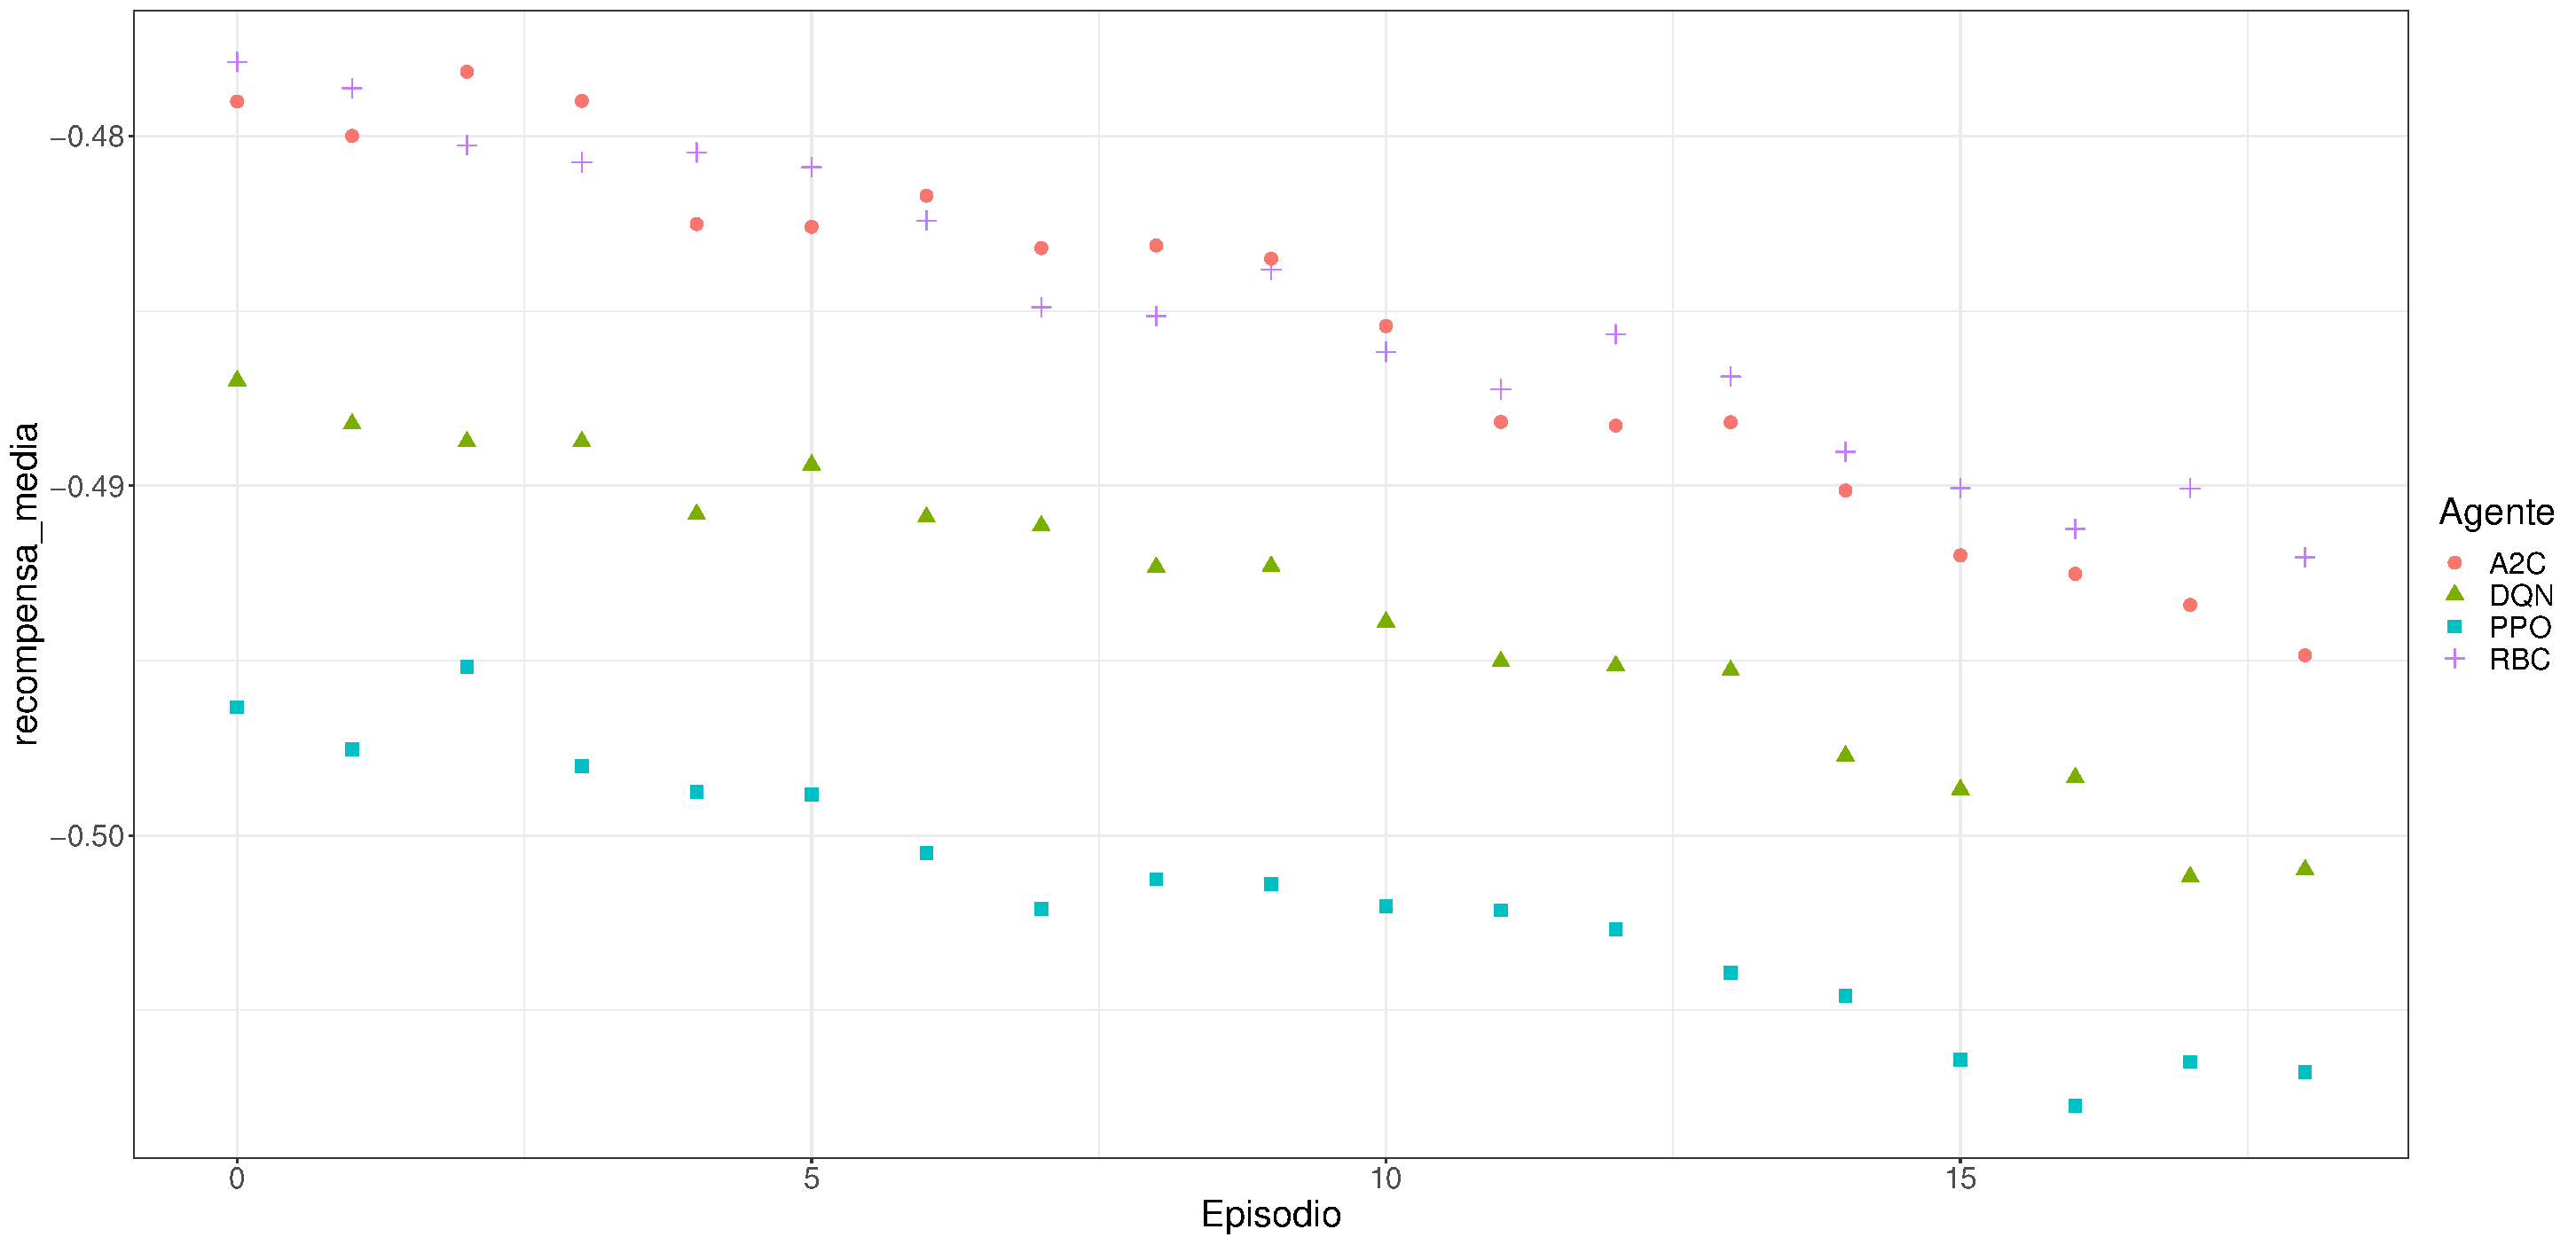
\includegraphics[width=\textwidth]{imagenes/recompensa-disc-hot.pdf}
    \caption{Ejemplo de la recompensa media obtenida en la validación de los agentes entrenados en el entorno \textit{discrete-stochastic-hot}}
    \label{fig:recompensa-disc-hot}
\end{figure}

\begin{figure}
    \centering
    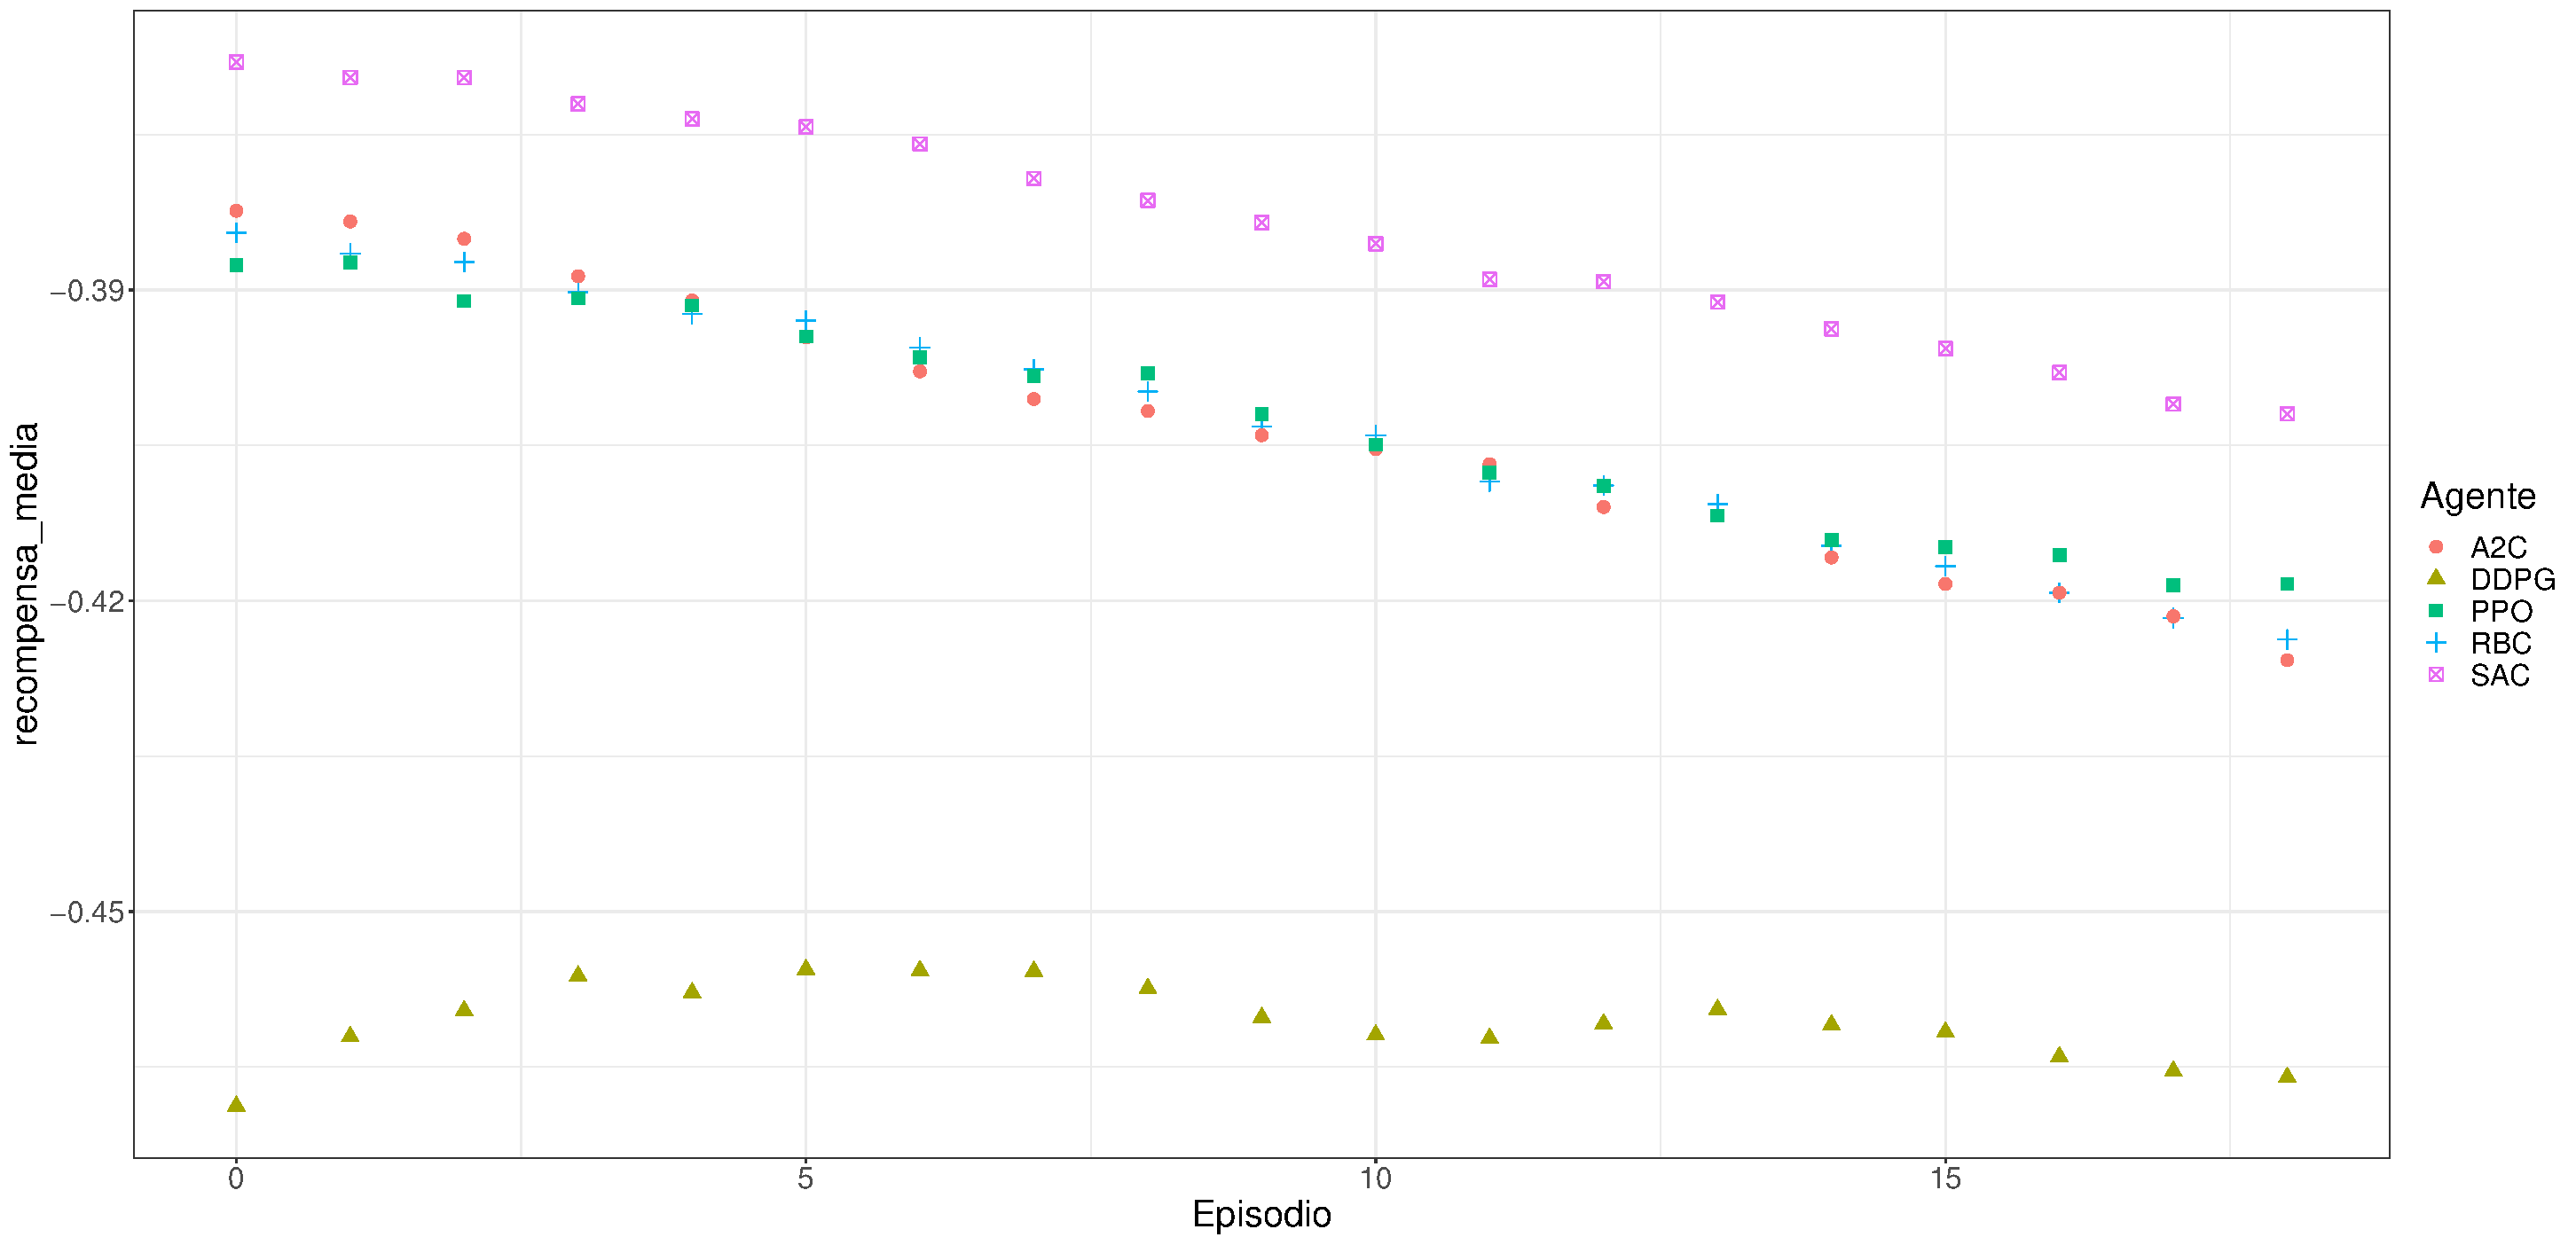
\includegraphics[width=\textwidth]{imagenes/recompensa-cont-hot.pdf}
    \caption{Ejemplo de la recompensa media obtenida en la validación de los agentes entrenados en el entorno \textit{continuous-stochastic-hot}}
    \label{fig:recompensa-cont-hot}
\end{figure}

\section{Experimentación avanzada}

Una vez estudiado el desempeño de los agentes en cada tipo de entorno, se llevaron a cabo una serie de experimentos adicionales destinados a comprender en profundidad otros aspectos del problema en cuestión. Dichos experimentos fueron realizados empleando el agente basado en DDPG, al tratarse de uno de los algoritmos que mejores resultados proporcionó en la mayoría de entornos y métricas de evaluación. El hecho de emplear DDPG frente a SAC se debió a que DDPG requirió menores tiempos de entrenamiento.

En las siguientes subsecciones se detallarán dichos experimentos y los resultados obtenidos.

\subsection{Equilibrio confort-consumo}
\label{sec:conf-con}

Como ya se estudió en la sección \ref{sec:formulacion}, el control HVAC por medio de RL supone el empleo de una función de recompensa que contemple tanto la maximización del confort como la reducción del consumo energético. Así, el objetivo a perseguir será la búsqueda del equilibrio entre ambas partes de la recompensa.

En la formulación del problema también abordamos cómo cada una de estas partes cuenta con una ponderación: $w_t$ y $(1-w_t)$; estos pesos nos permiten definir la importancia asignada al confort y al consumo, respectivamente, o lo que es lo mismo: su influencia en la función de recompensa.

Si atendemos a los experimentos llevados a cabo en la sección \ref{sec:evaluacion-agentes}, la importancia asignada a cada parte de la recompensa fue la misma, con $w_t=0.5$. De forma ilustrativa, pasemos ahora a asignar una mayor importancia al \textbf{consumo} y comparar los resultados obtenidos. Para llevar a cabo esta experimentación, emplearemos el agente basado en DDPG, en un clima templado y un espacio de acciones continuo.

Como se muestra en la Figura \ref{fig:pesos-consumo}, abogar por un 75\% de peso para el consumo (y, por tanto, un 25\% para el confort) frente a una ponderación equilibrada (50\%-50\%) supone:

\begin{itemize}
    \item Un menor consumo energético medio, ya que este toma una mayor importancia en la función de recompensa. Esto se observa especialmente bien si atendemos a la penalización por consumo, mucho menor para una ponderación 75\%-25\%.
    \item Un aumento de casi el 50\% de la violación del confort, debido a que el agente centra sus esfuerzos en reducir el consumo a toda costa. De nuevo, la penalización por confort es considerablemente mayor para el caso 75\%-25\%.
\end{itemize}

\begin{figure}
    \centering
    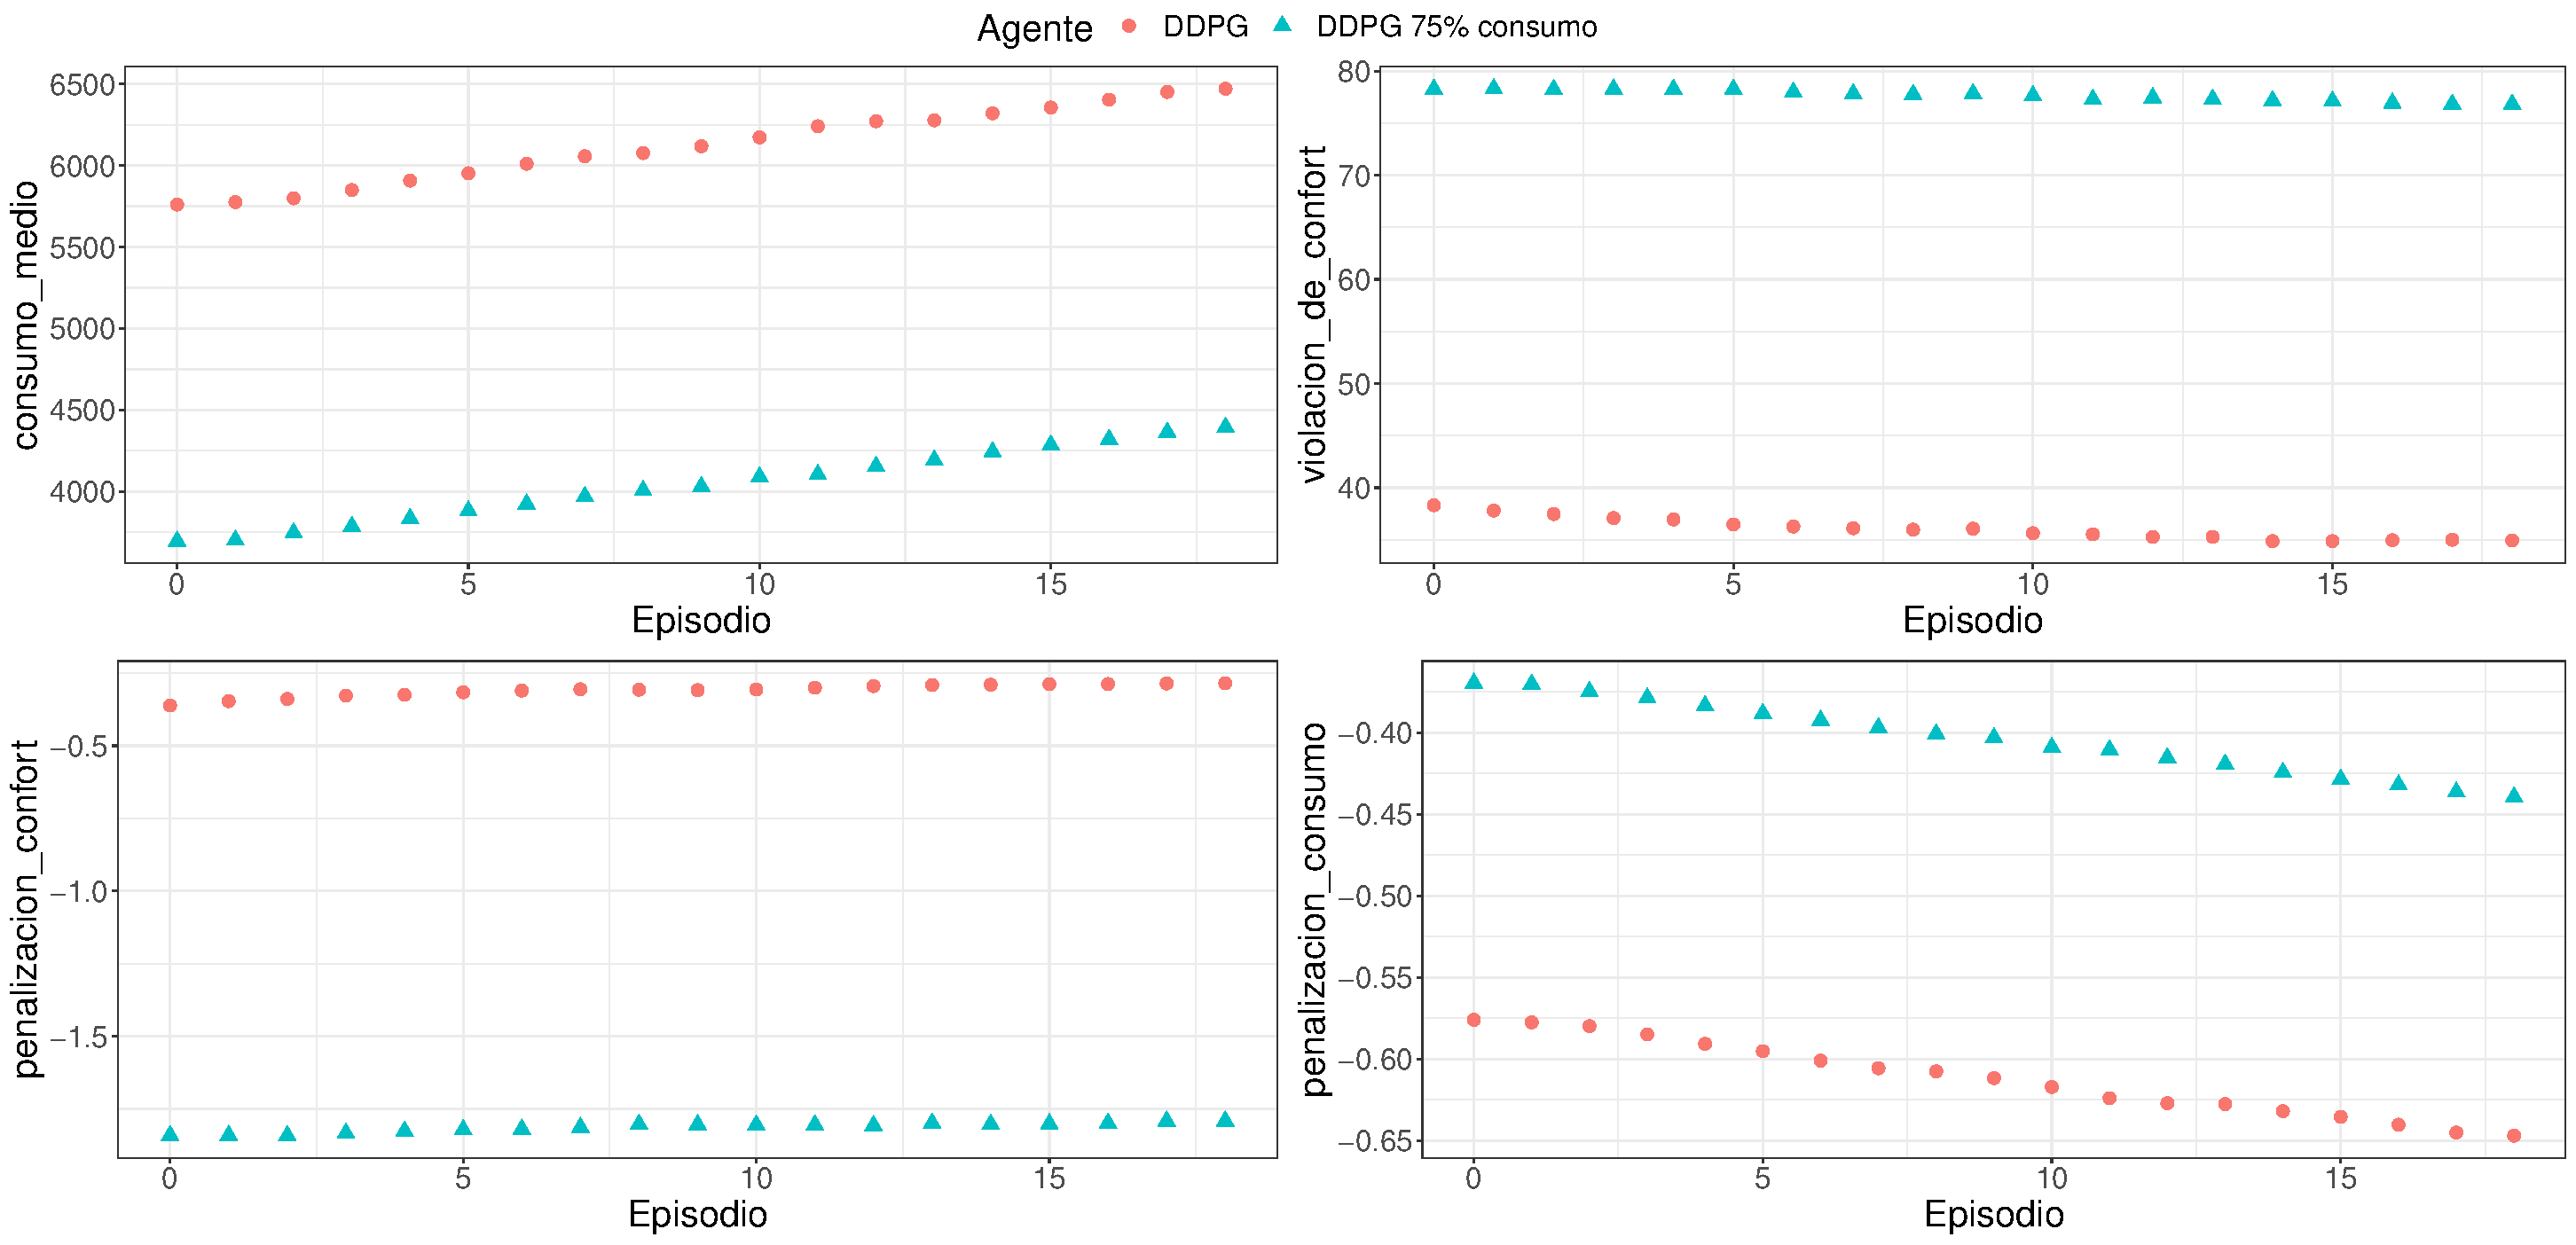
\includegraphics[width=\textwidth]{imagenes/energy-weights-DDPG.pdf}
    \caption{Resultados tras la validación de un agente entrenado con DDPG para diferentes ponderaciones de consumo}
    \label{fig:pesos-consumo}
\end{figure}

Con este ejemplo se ha tratado de ilustrar la flexibilidad que Energym nos ofrece a la hora de comparar diferentes ponderaciones de confort y consumo. Dichos pesos son un parámetro más a definir por el usuario, permitiendo una mayor personalización de los entornos y dotando a Energym de nuevas capacidades de experimentación. 

En conclusión, el equilibrio confort-consumo personalizable en Energym abre un amplio abanico de posibilidades, mayor aún si consideramos ponderaciones dinámicas o funciones de recompensa más complejas, fácilmente definibles a partir de los \textit{wrappers} ofrecidos por OpenAI Gym.

\subsection{Pruebas de robustez}
\label{sec:robustez}

Pasemos a estudiar la eficiencia de los agentes en entornos para los cuales no han sido entrenados. Estas ``pruebas de robustez'' nos permiten saber hasta qué punto un agente es capaz de generalizar y obtener un buen rendimiento en condiciones no experimentadas durante su entrenamiento.

Así, el experimento planteado consistirá en la evaluación de un agente entrenado en un clima \textbf{templado} en los entornos \textbf{cálido} y \textbf{frío}. Esto nos permitirá conocer la versatilidad de un agente entrenado en un clima con temperaturas más extremas.

Veamos, pues, los resultados obtenidos para cada prueba de robustez. De nuevo, utilizaremos el agente basado en DDPG en las mismas condiciones que la experimentación anterior.

Como podemos ver en la Figura \ref{fig:recompensa-robustez}, en un período de 20 episodios un agente entrenado en un clima templado ofrece un mejor control en un clima cálido que en uno mixto. Esto puede deberse a que el clima mixto supone una complejidad superior, al contar con un mayor rango de temperaturas a cubrir. No ocurre lo mismo para el agente entrenado en un entorno mixto y probado en uno frío. En comparación con el caso anterior, el bajo rendimiento podría deberse a que un clima templado es más próximo a las características del cálido que del frío, o bien que el clima frío requiera, por lo general, un mayor consumo energético.

\begin{figure}
    \centering
    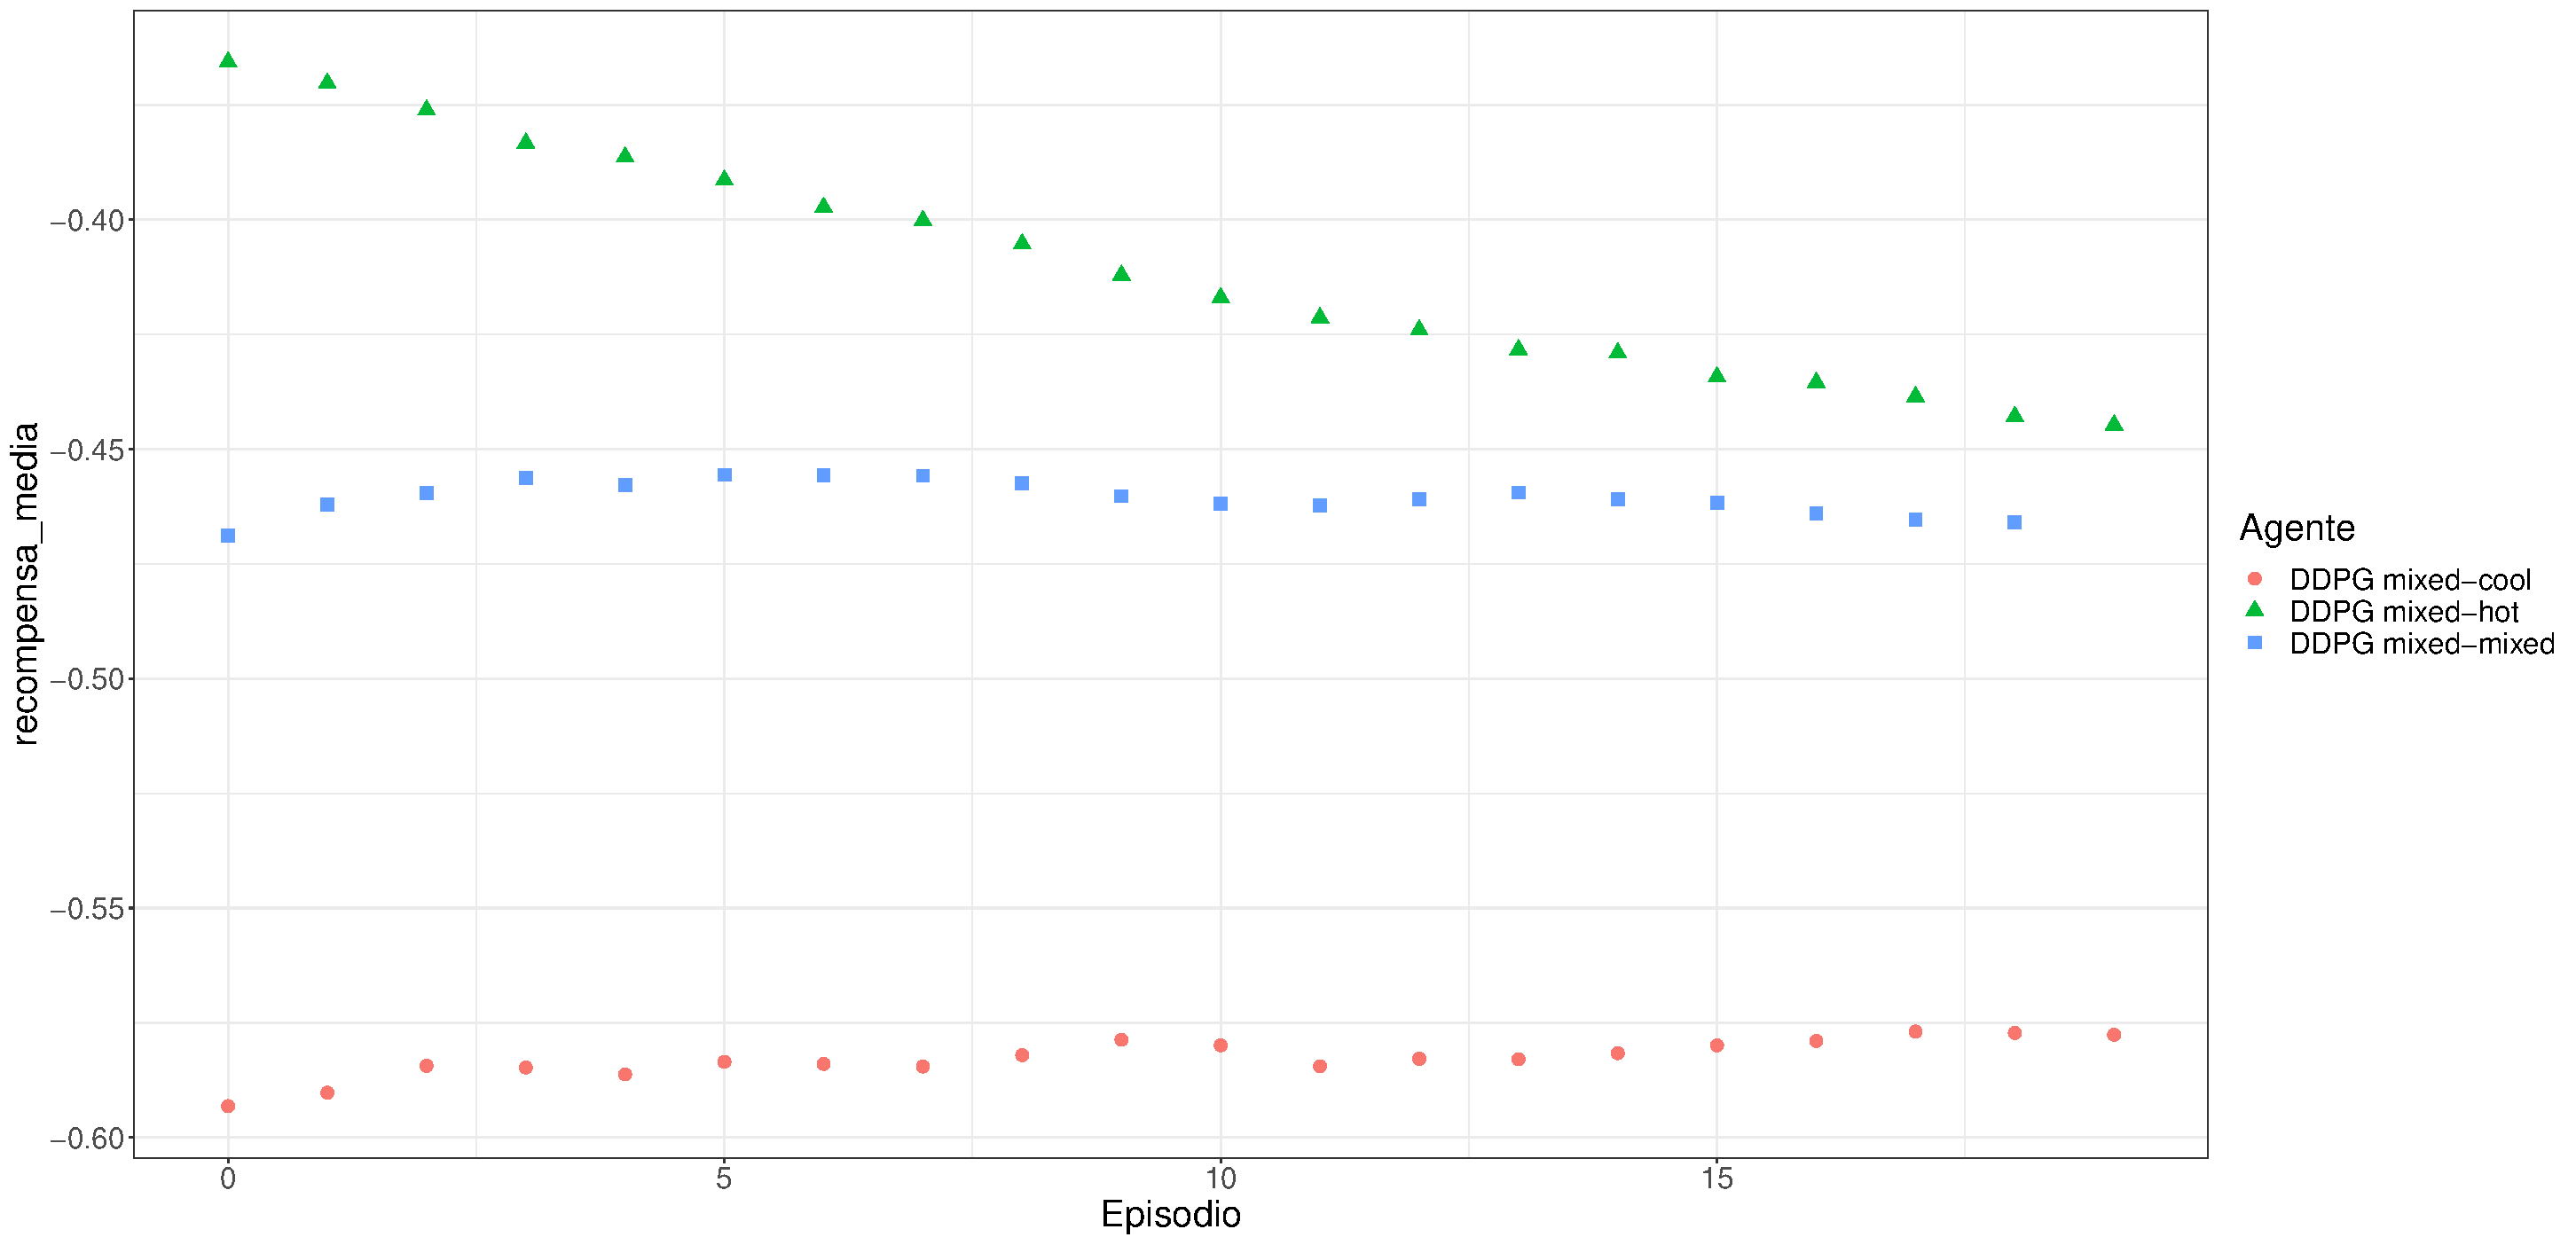
\includegraphics[width=\textwidth]{imagenes/recompensa-robustez.pdf}
    \caption{Evaluación del agente entrenado en clima \textit{mixed} y ejecutado en \textit{mixed}, \textit{cool} y \textit{hot}}
    \label{fig:recompensa-robustez}
\end{figure}

Este tipo de pruebas nos permiten conocer si el entrenamiento de un agente en un determinado tipo de entorno podría ser prescindible. Por ejemplo, en este caso, podríamos emplear el agente \textit{mixed} en el entorno \textit{hot} y obtendríamos mejores resultados, lo que reduce nuestro interés por entrenar un agente para cada entorno, pudiendo disponer de un único agente que opere bien en múltiples contextos.

A modo de reflexión, una discusión más profunda sobre los resultados ofrecidos por este tipo de experimentos sería un interesante debate a abordar de la mano de una persona experta en este campo. Aunque dicha discusión escapa de los objetivos de este proyecto, en esta sección hemos visto cómo Energym podría ser utilizado para un estudio en profundidad ante este tipo de situaciones.

\subsection{\textit{Curriculum learning}}
\label{sec:cv-learning}

En esta última sección abordaremos la aplicación de \textit{curriculum learning} en nuestro problema. Se trata de un tipo de aprendizaje progresivo, consistente en partir del entrenamiento en escenarios sencillos e ir utilizando el conocimiento adquirido hasta el momento para entrenarse en entornos más complejos.

Este método de aprendizaje ha demostrado ser de gran utilidad, logrando importantes avances en el ámbito del aprendizaje por refuerzo \cite{portelas2020automatic}. Se trata de un tipo de aprendizaje inspirado profundamente en cómo los humanos aprendemos, ya que nuestra formación se basa en un currículo de situaciones de aprendizaje interdependientes de diversa y progresiva complejidad \cite{narvekar2020curriculum}.

En el ámbito de nuestro problema, el aspecto fundamental que marca la complejidad de un entorno es la variabilidad de su clima: es mucho más fácil optimizar el control HVAC en un entorno donde las temperaturas apenas varían a lo largo del año, que en otro donde el clima es más inestable. Así, probaremos a comparar el rendimiento de un agente entrenado directamente sobre un clima \textit{mixed} con otro entrenado en los climas \textit{hot} y \textit{cool}. Utilizaremos DDPG bajo las mismas configuraciones descritas en los experimentos anteriores, siguiendo el proceso de aprendizaje detallado en la Figura \ref{fig:cv-learning}.

\begin{figure}
    \centering
    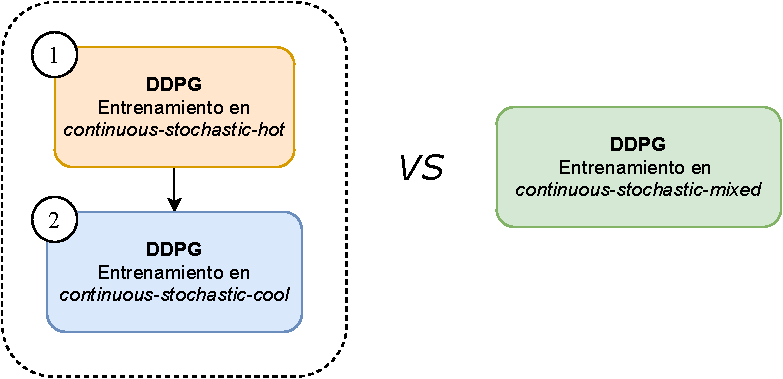
\includegraphics[width=\textwidth]{imagenes/cv-learning.pdf}
    \caption{Experimentación mediante \textit{curriculum learning}}
    \label{fig:cv-learning}
\end{figure}

Una vez realizado el experimento, si atendemos a la Figura \ref{fig:cv-learning-recompensa}  y la Tabla \ref{tb:cv-learning}, observamos que el agente entrenado en un entorno cálido y, posteriormente, en un entorno frío, es capaz de ofrecer mejores resultados que un agente entrenado en un entorno templado. Una posible explicación podría ser que el agente entrenado mediante \textit{curriculum learning} cuenta con una mayor especialización en temperaturas altas y bajas, en contraposición con el agente entrenado en \textit{mixed}, el cual no es capaz de gestionar temperaturas moderadamente fuera de su rango habitual.

\begin{figure}
    \centering
    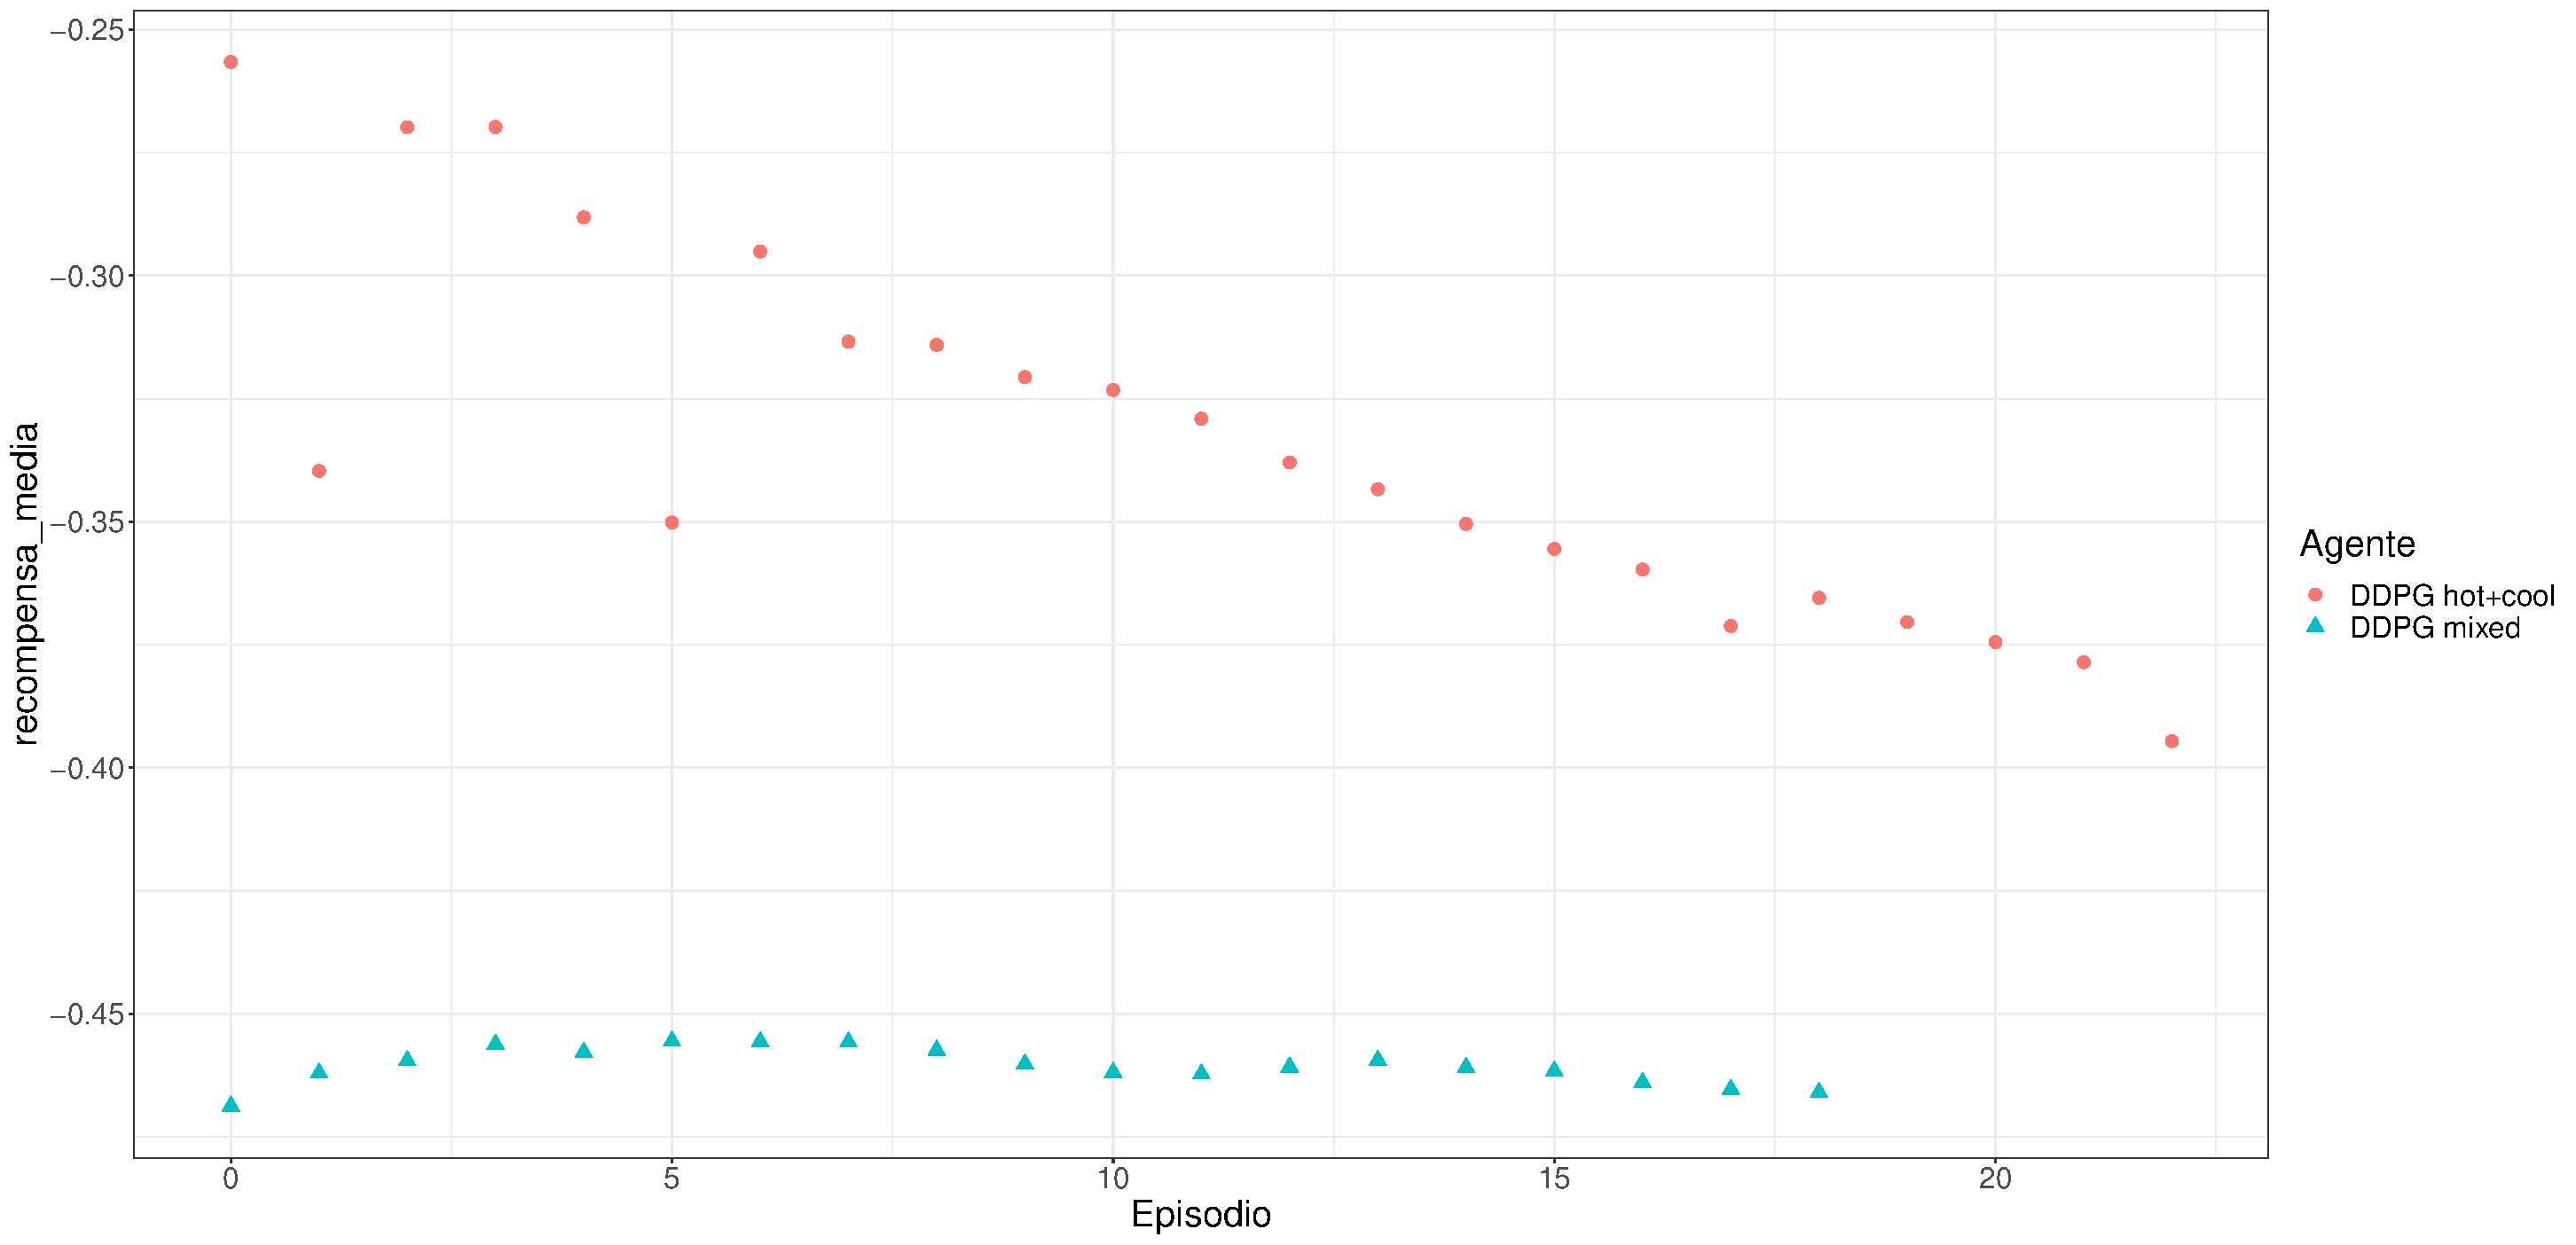
\includegraphics[width=\textwidth]{imagenes/recompensa-cv-learning.pdf}
    \caption{Recompensas medias obtenidas en la experimentación con \textit{curriculum learning}}
    \label{fig:cv-learning-recompensa}
\end{figure}

\begin{table}
    \centering
    \caption{Resultados obtenidos en la validación de DDPG entrenado en \textit{mixed} y DDPG entrenado en \textit{hot} y \textit{cool} sobre el entorno \textit{continuous-mixed}}
    \label{tb:cv-learning}
    \resizebox{\textwidth}{!}{%
    \begin{tabular}{ccccccc}
    \textbf{} & \multicolumn{2}{c}{\textbf{Recompensa}} & \multicolumn{2}{c}{\textbf{Consumo}} & \multicolumn{2}{c}{\textbf{Viol. confort}} \\ \hline
     & \textit{media} & \textit{desv} & \textit{media} & \textit{desv} & \textit{media} & \textit{desv} \\ \hline
    \textbf{DDPG mixed} & -.461 & .004 & 6118.94 & 234.366 & 36.044 & 1.063 \\ \hline
    \textbf{DDPG hot+cool} & \textbf{-.334} & .038 & \textbf{4396.529} & 542.063 & \textbf{34.683} & 2.81 \\ \hline
    \end{tabular}%
    }
\end{table}

Finalmente, se reitera en la idea de que la profundización en estos resultados podrían dar lugar a un amplio debate que va más allá de los objetivos de este trabajo. Así, el principal objetivo de esta sección ha sido demostrar cómo Energym puede ajustarse a un tipo de experimentaciones de mayor complejidad que se alejan de las pruebas convencionales, y que, sin duda alguna, cuentan con un enorme potencial en este campo.


\chapter{Conclusiones}
\label{ch:5}

En este último capítulo quedan resumidas las principales aportaciones de este trabajo, haciendo especial énfasis en la consecución de los objetivos propuestos y los resultados obtenidos. Finalmente, se detallarán posibles trabajos futuros, así como las principales lecciones aprendidas tras realizar este proyecto.

\section{Conclusiones}

Este trabajo ha tratado de aportar soluciones a un problema aún abierto como es el de la aplicación de RL/DRL en el control óptimo de sistemas HVAC. Se trata de un campo repleto de posibilidades, y que sin duda seguirá creciendo en popularidad en los próximos años.

El desarrollo de Energym es un primer paso hacia la estandarización de este campo, un pilar fundamental de cara a poder estudiar y adoptar las mejores soluciones en control HVAC, garantizando así la reducción del consumo energético y el bienestar de las personas. Se trata de una idea pionera, funcional y que responde a las necesidades expresadas por la comunidad científica.

Por otro lado, la experimentación llevada a cabo en este proyecto pretende, no sólo demostrar la eficacia de Energym como entorno de ejecución de simulaciones energéticas, sino también evidenciar la profundidad y complejidad que supone este problema. Así, en el marco de este proyecto, hemos visto una pequeña parte de la inmensa cantidad de configuraciones, variables y técnicas que pueden afectar al rendimiento de los algoritmos de RL/DRL en control HVAC, abriendo la puerta a futuros trabajos que aprovechen el potencial de Energym en diferentes ámbitos de aplicación. 

A su vez, tanto la herramienta desarrollada como el conocimiento adquirido a lo largo de este proyecto permiten plantear cuestiones sobre aspectos hasta el momento asumidos, como la efectividad de las funciones de recompensa expuestas en la literatura, o la capacidad de generalización de modelos entrenados en condiciones muy concretas. Así, Energym pretende arrojar luz sobre algunas de estas cuestiones y servir como un marco de pruebas estándar sobre el que poder corroborar diferentes hipótesis.

Un aspecto a considerar es cómo este tipo de soluciones de control podrían ser aplicadas de forma exitosa en entornos reales, dada su complejidad en comparación con los entornos simulados, donde las variables que influyen en el control se encuentran perfectamente identificadas. Atendiendo a la literatura, existen limitadas aplicaciones reales basadas en métodos de RL \cite{costanzo2016experimental,wang2020reinforcement} y menos aún que hagan uso de algoritmos de DRL \cite{wang2020reinforcement}. Se trata, pues, de un problema abierto y complejo, para el cual no se cuenta con suficientes aportaciones como para poder ofrecer una respuesta precisa. Así, un objetivo a largo será que el número de soluciones probadas en entornos reales aumente a medida que este campo alcance su madurez.

Otro factor de relevancia son los tiempos de entrenamiento requeridos por este tipo de agentes, crecientes a medida que la complejidad y los escenarios contemplados aumentan. Esto pone en riesgo la escalabilidad de estos sistemas, siendo una posible solución un primer entrenamiento estático que permita ubicar al modelo en el entorno y un posterior entrenamiento \textit{online} que responda a cambios menores \cite{azuatalam2020reinforcement}.

Finalmente, la búsqueda de dicha escalabilidad ha empujado al desarrollo de este campo desde la perspectiva de los sistemas multiagente \cite{nagarathinam2020marco,yu2020multi,li2015multi}, ofreciendo un control HVAC descentralizado y flexible entre diferentes agentes independientes. Se trata de una idea prometedora y bastante reciente, de la cual cabe esperar importantes avances en los próximos años.

\section{Cobertura de objetivos}

A continuación, abordaremos la consecución de los diferentes objetivos planteados al inicio de este proyecto:

\begin{tcolorbox}[colbacktitle=green!30!white, title=Subobjetivo 1, coltitle=black, fonttitle=\bfseries]
Comprensión de los fundamentos del aprendizaje por refuerzo y su aplicación en control HVAC.
\end{tcolorbox}

En el Capítulo \ref{ch:2} se han presentado los fundamentos del aprendizaje por refuerzo y aprendizaje profundo por refuerzo, así como gran parte de los algoritmos que conforman el estado del arte. Posteriormente, se ha abordado su aplicabilidad en el ámbito del control HVAC, presentando el marco formal empleado para definir este problema.

Finalmente, se han descrito diferentes aplicaciones de RL/DRL en control HVAC presentes en la literatura, evidenciando las motivaciones que impulsaron el desarrollo de este proyecto.

\begin{tcolorbox}[colbacktitle=green!30!white, title=Subobjetivo 2, coltitle=black, fonttitle=\bfseries]
Extensión de la librería Python \href{https://github.com/jajimer/energym}{Energym} haciendo uso de la herramienta \href{https://gym.openai.com/}{Gym} de OpenAI.
\end{tcolorbox}

En el Capítulo \ref{ch:3} se ha descrito el conjunto de actividades llevadas a cabo en el desarrollo de Energym como parte de un equipo de trabajo profesional. Dichas tareas han supuesto la extensión de las funcionalidades de Energym, adaptándolo a diferentes entornos de simulación y facilitando su integración con librerías de DRL como Stable Baselines3.

Todo este proceso de implementación ha estado completamente ligado a la interfaz de programación para entornos de RL que ofrece OpenAI Gym, aprovechando las ventajas que esta herramienta ofrece para desarrollar Energym de una forma estandarizada y escalable.

\begin{tcolorbox}[colbacktitle=green!30!white, title=Subobjetivo 3, coltitle=black, fonttitle=\bfseries]
Entrenamiento monitorizado de diferentes algoritmos de DRL disponibles en \href{https://github.com/DLR-RM/stable-baselines3}{Stable Baselines3} haciendo uso de las herramientas \href{https://tensorflow.org/tensorboard}{TensorBoard} y \href{https://mlflow.org/}{MLflow}.
\end{tcolorbox}

En el Capítulo \ref{ch:4} se abordó el uso de múltiples algoritmos de DRL disponibles en Stable Baselines3 en combinación con Energym para ilustrar su aplicación en control HVAC. Esto supuso el entrenamiento y ejecución de los agentes en diferentes entornos y condiciones de simulación (espacios de acciones, climas...) de cara a evaluar y comparar los resultados obtenidos.

Por otro lado, este proceso fue continuamente monitorizado haciendo uso de las herramientas TensorBoard y MLflow. La primera sirvió para monitorizar el aprendizaje, mientras que la segunda sirvió para registrar los experimentos realizados y sus configuraciones. Todo el proceso de integración de Energym con estas herramientas quedó detallado en el Capítulo \ref{ch:3}.

\begin{tcolorbox}[colbacktitle=green!30!white, title=Subobjetivo 4, coltitle=black, fonttitle=\bfseries]
Comparativa de los resultados obtenidos para cada uno de los agentes en diferentes contextos de clima y espacios de acciones (discreto y continuo).
\end{tcolorbox}

La sección \ref{sec:results} del Capítulo \ref{ch:4} detalla los resultados obtenidos tras la experimentación con diferentes algoritmos de DRL en combinación con Energym. En los entornos discretos, ningún agente logró superar de forma significativa el rendimiento de un agente basado en reglas, siendo A2C el algoritmo que consiguió obtener los resultados más similares. 

Por otro lado, en los entornos continuos sí que se lograron importantes mejoras con respecto al agente basado en reglas, siendo SAC y DDPG los algoritmos que ofrecieron mejores resultados. De esta forma, queda demostrada la posibilidad de superar el rendimiento de un agente basado en reglas haciendo uso de un control HVAC basado en DRL.

\begin{tcolorbox}[colbacktitle=green!30!white, title=Subobjetivo 5, coltitle=black, fonttitle=\bfseries]
Estudio de la recompensa obtenida por un agente en función de la importancia asignada a confort y consumo energético.
\end{tcolorbox}

Dentro de los experimentos avanzados llevados a cabo en el Capítulo \ref{ch:4} (sección \ref{sec:conf-con}), se estudió la influencia de las ponderaciones de consumo y confort en la función de recompensa empleada por los agentes de DRL. 

El ejemplo ilustrativo mostrado en esta sección, planteó cómo un agente con un mayor énfasis en la reducción del consumo energético es capaz de consumir menos a costa de un mayor número penalizaciones por violación de confort.

\begin{tcolorbox}[colbacktitle=green!30!white, title=Subobjetivo 5, coltitle=black, fonttitle=\bfseries]
Ejecución de pruebas de robustez que permitan conocer el rendimiento de los agentes en diferentes climas a los empleados como entrenamiento.
\end{tcolorbox}

En la sección \ref{sec:robustez} del Capítulo \ref{ch:4} se evaluaron diferentes situaciones en las que un agente era ejecutado en un entorno diferente al empleado en su entrenamiento. Así, las pruebas realizadas revelaron que un agente entrenado en un entorno templado (\textit{mixed}) es capaz de ofrecer muy buenos resultados en un clima cálido, no ocurriendo lo mismo en un clima frío, donde dicho rendimiento disminuye.

\begin{tcolorbox}[colbacktitle=green!30!white, title=Subobjetivo 5, coltitle=black, fonttitle=\bfseries]
Aplicación de \textit{curriculum learning} con diferentes agentes y análisis de los resultados obtenidos.
\end{tcolorbox}

Finalmente, en la sección \ref{sec:cv-learning} del Capítulo \ref{ch:4} se ilustró la aplicación de \textit{curriculum learning} en el ámbito de este problema. El ejemplo planteado mostró cómo un agente entrenado progresivamente a partir de los entornos \textit{hot} y \textit{cool} es capaz de ofrecer un mejor rendimiento que un agente entrenado únicamente en un entorno \textit{mixed}.

\section{Trabajo futuro}
\label{sec:trabajo-futuro}

Son muchas las posibilidades y líneas de trabajo que pueden derivarse de este proyecto. Como hemos podido ver a lo largo de su desarrollo, la cantidad de técnicas, configuraciones, entornos o climas a emplear abren la puerta a un sinfín de experimentos de relevancia en el campo. A continuación, se propone un listado de algunas de las principales metas planteadas como trabajo futuro\footnote{Muchas de estas posibles mejoras se encuentran descritas en el listado de \textit{issues} del repositorio de Energym: \url{https://github.com/jajimer/energym/issues}.}:

\begin{itemize}
    \item Ampliación de la compatibilidad de Energym con otros entornos de simulación como \href{https://www.openmodelica.org/}{OpenModelica} o \href{https://es.mathworks.com/products/simulink.html}{Simulink}.
    \item Experimentación con otros entornos, climas y variables. Actualmente se encuentra en proceso la integración de Energym en el entorno  \href{https://github.com/NREL/EnergyPlus/blob/v8.6.0/testfiles/2ZoneDataCenterHVAC_wEconomizer.idf}{Data Center}, el cual incluye como variables de entrada tanto los \textit{setpoints} de calefacción y refrigeración como la ventilación del edificio.
    \item Implementación de entornos con espacios de acciones multidiscretos, así como ampliación del espacio de acciones empleado por los entornos discretos.
    \item Evaluación de otros algortimos de DRL implementados tanto en Stable Baselines3 (por ejemplo, TD3) como en otras librerías como \href{https://docs.ray.io/en/master/rllib.html}{RLlib}, \href{https://www.tensorflow.org/agents}{TensorFlow Agents} o \href{https://github.com/keras-rl/keras-rl}{Keras-RL}.
    \item Comparar los resultados obtenidos para diferentes funciones de recompensa, así como implementar ponderaciones dinámicas (por ejemplo, variables en el tiempo o dependientes del número de personas en el edificio) para consumo y confort.
    \item Profundización en el uso de \textit{curriculum learning}, estudiando la capacidad de generalización en diferentes entornos donde no sólo cambia el clima sino también las características del edificio.
    \item Realización de pruebas de robustez adicionales que permitan cubrir todo el espacio de combinaciones climáticas posibles.
    \item Extensión de las funcionalidades de Energym para el procesamiento y representación automática de los datos generados.
    \item Entrenamiento y ejecución de los agentes en la nube, haciendo uso de servicios como \href{https://cloud.google.com/}{Google Cloud}, \href{https://azure.microsoft.com/}{Microsoft Azure} o \href{https://aws.amazon.com/}{Amazon Web Services}.
\end{itemize}

Tras la conclusión de este proyecto, un objetivo a corto plazo será dar conocer Energym y sus aplicaciones mediante publicaciones científicas en revistas especializadas en este campo, favoreciendo así su difusión y madurez. Esta labor se enmarca dentro del proyecto \href{https://jgromero.github.io/proficient/}{PROFICIENT}, financiado por el programa \textit{EXPLORA} del Ministerio de Ciencia, Innovación y Universidades (TIN2017-91223-EXP) y orientado al desarrollo de soluciones basadas en DRL para el control energético eficiente de edificios.

\section{Valoración personal}

Realizar un trabajo de fin de máster que involucrase la profundización en el campo del aprendizaje por refuerzo fue una de las principales motivaciones a adentrarme de lleno en este proyecto. A su vez, el hecho de poder aunar mi interés por este campo y su aplicación en la resolución de problemas reales fueron motivos de peso para decantarme por un trabajo de tal envergadura. 

Considero al aprendizaje por refuerzo como un paradigma de enorme potencial, en ocasiones eclipsado por el aprendizaje supervisado y no supervisado, pero que en los últimos años ha conseguido una gran repercusión gracias a las aportaciones y popularidad de proyectos como \href{https://deepmind.com/research/case-studies/alphago-the-story-so-far}{AlphaGo} o \href{https://deepmind.com/blog/article/alphazero-shedding-new-light-grand-games-chess-shogi-and-go}{AlphaZero}. Actualmente contamos con aplicaciones de RL en inmensidad de ámbitos de lo más diversos, siendo el control energético un dominio llamativo y de especial relevancia para la sociedad.

Desde una perspectiva personal, el uso de RL en el control de sistemas HVAC abre la puerta a una nueva forma mucho más eficiente de garantizar el bienestar de las personas. Si a un control eficiente de estos sistemas sumásemos fuentes de energía renovables, contaríamos con edificios energéticamente autorregulados y sostenibles, algo prioritario ante la amenaza del cambio climático y el calentamiento global.
 
Finalmente, considero que las aportaciones de este trabajo podrán ser especialmente relevantes para la comunidad científica involucrada en este ámbito. El desarrollo de Energym y la experimentación propuesta en este trabajo abogan por una visión común y unificada de las propuestas que conforman el estado del arte en control HVAC y RL, facilitando el progreso, la reproducibilidad y la estandarización de las soluciones existentes y aún por desarrollar.




\printbibliography

\newpage
% \nocite{*}

%% Apendices
%\appendix
%\input{apendices/...}

\chapter*{}
\thispagestyle{empty}

\end{document}
